\documentclass[a4paper,12pt]{article}

\usepackage[T1]{fontenc}
\usepackage[italian]{babel}
\usepackage{graphicx}
\usepackage{geometry}
\usepackage{tabularx}
\usepackage{longtable}
\usepackage[table]{xcolor}
\usepackage[most]{tcolorbox}
\usepackage{fancyhdr}
\usepackage[hidelinks]{hyperref}
\usepackage{float}
\usepackage{enumitem}

\setcounter{secnumdepth}{5}   
\setcounter{tocdepth}{5}     
\renewcommand{\theparagraph}{\thesubsubsection.\arabic{paragraph}}

\newcommand{\groupmail}{alittlebyte.swe@gmail.com}
\newcommand{\grouplogo}{../../.github/site-src/assets/logo_alittlebyte.png}
\newcommand{\groupsymbol}{../../.github/site-src/assets/solo_logo.png}

\geometry{
    left=2.5cm,
    right=2.5cm,
    top=2.5cm,
    bottom=2.5cm,
    headheight=331pt,
    includeheadfoot
}

\pagestyle{fancy}
\fancyhf{}

\renewcommand{\headrulewidth}{0pt}
\fancyhead{}

\renewcommand{\footrulewidth}{0.4pt}
\fancyfoot[L]{\includegraphics[height=0.6cm]{\groupsymbol}\hspace{0.45em}aLittleByte}
\fancyfoot[R]{Analisi dei Requisiti}

\fancypagestyle{firstpage}{
    \fancyhf{}
    \renewcommand{\headrulewidth}{0pt}
    \renewcommand{\footrulewidth}{0.4pt}
    \fancyhead[C]{%
        \makebox[\textwidth][c]{%
            \begin{tabular}{c}
                \includegraphics[height=10cm]{\grouplogo}\\[1ex]
                \small\texttt{\groupmail}
            \end{tabular}%
        }
    }
    \fancyfoot[L]{\includegraphics[height=0.6cm]{\groupsymbol}\hspace{0.45em}aLittleByte}
    \fancyfoot[R]{Analisi dei Requisiti}
}

\providecommand{\glslink}[2]{\href{https://alittlebyte-19.github.io/Documentazione/glossario.html\#gls-#1}{\underline{#2}\textsuperscript{\scriptsize G}}}

\begin{document}

\thispagestyle{firstpage}

\vspace*{0.5cm}

\begin{center}
    {\LARGE \textbf{Analisi dei Requisiti}}
\end{center}

\vspace{1.5cm}

\begin{center}
    \renewcommand{\arraystretch}{1.3}
    \begin{tcolorbox}[
        width=0.92\textwidth,
        colback=gray!6,
        colframe=gray!45,
        boxrule=0.5pt,
        arc=2mm,
        boxsep=0pt,
        left=8pt, right=8pt, top=8pt, bottom=8pt
    ]
        \begin{tabularx}{\linewidth}{>{\bfseries}p{3.5cm} X}
            Gruppo      & aLittleByte (gruppo 19) \\
            Versione    & 1.0.0 \\
            Redattori   & Angela Maule, Angelica Gastaldello, Vinicius Yuri Kaneda Fernandes, Leonardo Soligo, Eleonora Bellet, Diego Belluz, Alex Oloni\\
            Verificatori& Angela Maule, Eleonora Bellet, Diego Belluz, Vinicius Yuri Kaneda Fernandes\\
            Destinatari & Prof. Tullio Vardanega, Prof. Riccardo Cardin \\
            Data        & 27/05/2026\\
        \end{tabularx}
    \end{tcolorbox}
\end{center}

\newpage

\newgeometry{left=2.5cm,right=2.5cm,top=2.5cm,bottom=2.5cm,includefoot}

\begin{center}
    {\Large \textbf{Registro delle Modifiche}}
\end{center}

\vspace{0.35cm}

\renewcommand{\arraystretch}{1.35}
{\small
\setlength{\LTleft}{0pt}
\setlength{\LTright}{0pt}
\begin{longtable}{|p{1.2cm}|p{1.9cm}|p{4.3cm}|p{2.8cm}|p{2.1cm}|p{2.1cm}|}
    \hline
    \rowcolor{gray!20}
    \textbf{Versione} & \textbf{Data} & \textbf{Descrizione} & \textbf{Redattore} & \textbf{Verificatore} & \textbf{Approvatore} \\
    \hline
    \endfirsthead
    \hline
    \rowcolor{gray!20}
    \textbf{Versione} & \textbf{Data} & \textbf{Descrizione} & \textbf{Redattore} & \textbf{Verificatore} & \textbf{Approvatore} \\
    \hline
    \endhead
    1.0.0 & 27/05/2026 & Approvazione versione 1.0.0 & - & - & Leonardo Soligo \\
    \hline
    \rowcolor{gray!8} 0.15.4 & 17/05/2026 & Correzione requisiti (coerenza RF e UC) & Angela Maule & Diego Belluz & - \\
    \hline
    0.15.3 & 12/05/2026 & Tracciamento casi d'uso (matrici UC->RF) & Angela Maule & Eleonora Bellet & - \\
    \hline
    0.15.2 & 10/05/2026 & Requisiti di qualita' e vincolo (nuova sezione) & Angelica Gastaldello & V.Y. Kaneda Fernandes & - \\
    \hline
    \rowcolor{gray!8} 0.15.1 & 09/05/2026 & Requisiti funzionali (prima stesura RF) & Angela Maule & Eleonora Bellet & - \\
    \hline
    0.15.0 & 07/05/2026 & UC-19 (scenari e relazioni) & Yuri Kaneda Fernandes & V.Y. Kaneda Fernandes & - \\
    \hline
    \rowcolor{gray!8} 0.14.0 & 05/05/2026 & UC-18 (scheda e diagramma) & Leonardo Soligo & Eleonora Bellet & - \\
    \hline
    0.13.0 & 03/05/2026 & UC-17 (scheda e scenari) & Eleonora Bellet & V.Y. Kaneda Fernandes & - \\
    \hline
    \rowcolor{gray!8} 0.12.1 & 02/05/2026 & Diagrammi UC-15, UC-16 (figure UML) & Eleonora Bellet & Eleonora Bellet & - \\
    \hline
    0.12.0 & 30/04/2026 & UC-16 (dettaglio modifica metadati) & Angelica Gastaldello & V.Y. Kaneda Fernandes & - \\
    \hline
    \rowcolor{gray!8} 0.11.0 & 28/04/2026 & UC-15 (storico e dettaglio) & Angela Maule & Eleonora Bellet & - \\
    \hline
    \rowcolor{gray!8} 0.10.1 & 25/04/2026 & Diagrammi UC-12/13/14 (figure UML) & Yuri Kaneda Fernandes & V.Y. Kaneda Fernandes & - \\
    \hline
    0.10.0 & 24/04/2026 & UC-12/13/14 (filtri di ricerca) & Diego Belluz & Eleonora Bellet & - \\
    \hline
    \rowcolor{gray!8} 0.9.0 & 21/04/2026 & UC-10/11 (filtro storico) & Angelica Gastaldello & V.Y. Kaneda Fernandes & - \\
    \hline
    \rowcolor{gray!8} 0.8.0 & 17/04/2026 & UC-8/9 (upload con metadati e storico) & Yuri Kaneda Fernandes & Eleonora Bellet & - \\
    \hline
    0.7.0 & 14/04/2026 & UC-7 (upload documento) & Diego Belluz & V.Y. Kaneda Fernandes & - \\
    \hline
    0.6.3 & 12/04/2026 & Correzione UC-5/6 (allineamento testo) & Alex Oloni & Angela Maule & - \\
    \hline
    \rowcolor{gray!8} 0.6.2 & 11/04/2026 & UC-6 (export dati) & Leonardo Soligo & V.Y. Kaneda Fernandes & - \\
    \hline
    0.6.1 & 10/04/2026 & UC-5 (reportistica) & Alex Oloni & Angela Maule & - \\
    \hline
    \rowcolor{gray!8} 0.6.0 & 09/04/2026 & UC-3/4 (attori e flussi) & Yuri Kaneda Fernandes & V.Y. Kaneda Fernandes & - \\
    \hline
    0.5.1 & 08/04/2026 & Diagrammi UC-1/2 (figure UML) & Leonardo Soligo & Angela Maule & - \\
    \hline
    \rowcolor{gray!8} 0.5.0 & 03/04/2026 & UC-1/2 (generazione contenuti) & Angela Maule & V.Y. Kaneda Fernandes & - \\
    \hline
    0.4.0 & 01/04/2026 & Attori del sistema (definizione iniziale) & Alex Oloni & Angela Maule & - \\
    \hline
    \rowcolor{gray!8} 0.3.0 & 31/03/2026 & Sezione introduttiva (scopo e riferimenti) & Leonardo Soligo & Angela Maule & - \\
    \hline
    0.2.0 & 31/03/2026 & Descrizione del prodotto (obiettivi e funzioni) & Angelica Gastaldello & V.Y. Kaneda Fernandes & - \\
    \hline
    \rowcolor{gray!8} 0.1.0 & 30/03/2026 & Struttura del documento (prima impostazione) & Angelica Gastaldello & Angela Maule & - \\
    \hline
\end{longtable}
}
\newpage

\tableofcontents

\newpage
\listoffigures
\newpage
\listoftables
\pagenumbering{arabic}
\setcounter{page}{5}
\fancyfoot[R]{Analisi dei Requisiti\hspace{0.8em}\thepage}
\newpage
\section{Introduzione}
\subsection{Scopo del documento}
Il presente documento di \glslink{analisi-dei-requisiti-adr}{Analisi dei Requisiti} ha l'obiettivo di descrivere in modo completo e strutturato i requisiti funzionali e non funzionali del sistema software progettato per il \glslink{committente-proponente}{proponente} Eggon S.r.l. .\\
L'applicazione implementerà i moduli "\glslink{ai-assistant-generativo}{AI Assistant Generativo}" e "\glslink{intelligenza-artificiale-ai}{AI} Co-Pilot per i Consulenti del Lavoro", permettendo di sperimentare le funzionalità previste in un ambiente controllato.\\
Il documento descrive in dettaglio i casi d'uso del sistema, che rappresentano la base per l'individuazione dei requisiti, e include i diagrammi dei casi d'uso per rappresentare visivamente le interazioni tra gli attori e il sistema. \\
I requisiti identificati costituiscono il riferimento per le attività di progettazione, sviluppo e collaudo dell'applicazione, garantendo coerenza con le esigenze del \glslink{committente-proponente}{committente} e con gli obiettivi formativi e tecnici del progetto. \\
Il documento è destinato a sviluppatori, progettisti e \glslink{stakeholder}{stakeholder}, fornendo una base condivisa per tutte le fasi del ciclo di vita del software.
Il documento non tratta nel dettaglio le scelte implementative o tecnologiche di basso livello, le quali saranno affrontate nelle successive fasi di progettazione architetturale.

\subsection{Sviluppo del documento}
Il presente documento è stato redatto adottando un \glslink{approccio-incrementale}{approccio incrementale}, con l’obiettivo di consentire aggiornamenti e revisioni nel corso del progetto.\\
La struttura e i contenuti sono stati definiti in modo da garantire flessibilità, permettendo di recepire eventuali modifiche derivanti dall’evoluzione dei requisiti o dal confronto con il \glslink{committente-proponente}{committente}.\\
Il documento è pertanto soggetto a un processo di revisione continua, finalizzato a mantenerne coerenza, completezza e allineamento con gli obiettivi progettuali.

\subsection{Riferimenti}
\subsubsection{Riferimenti normativi}
\begin{itemize}
    \item \textbf{\glslink{capitolato}{Capitolato} d'appalto C5 - \glslink{nexum}{NEXUM} (Eggon):}\\
    \url{https://www.math.unipd.it/~tullio/IS-1/2025/Progetto/C5.pdf}

    \item \textbf{\glslink{norme-di-progetto}{Norme di Progetto}:}\\
    Documento interno del gruppo \textit{aLittleByte} che definisce le regole, i ruoli e le procedure operative.\\
    \url{https://alittlebyte-19.github.io/Documentazione/RTB/Norme%20di%20Progetto/Norme%20di%20Progetto.pdf}

    \item \textbf{Regolamento del progetto didattico:}\\
    \url{https://www.math.unipd.it/~tullio/IS-1/2025/Dispense/PD1.pdf}
\end{itemize}
\subsubsection{Riferimenti informativi}
\begin{itemize}
    \item \textbf{\glslink{glossario}{Glossario}:}\\
    Documento interno del gruppo \textit{aLittleByte} contenente le definizioni dei termini tecnici.\\
    \url{https://alittlebyte-19.github.io/Documentazione/RTB/Glossario/Glossario.pdf}

    \item \textbf{Standard ISO/IEC 12207:1995:}\\
    \textit{Information technology -- Software life cycle processes}.\\
    \url{https://www.math.unipd.it/~tullio/IS-1/2009/Approfondimenti/ISO_12207-1995.pdf}

    \item \textbf{Standard ISO/IEC 9126:}\\
    \textit{Software engineering -- Product quality}.\\
    \url{https://it.wikipedia.org/wiki/ISO/IEC_9126}

    \item \textbf{Slide T07 - Qualità del software:}\\
    \url{https://www.math.unipd.it/~tullio/IS-1/2025/Dispense/T07.pdf}\\

    \item \textbf{Slide T08 - Qualità del software:}\\
    \url{https://www.math.unipd.it/~tullio/IS-1/2025/Dispense/T08.pdf}\
\end{itemize}

\section{Descrizione del prodotto}

\subsection{Obiettivi del prodotto}

L'obiettivo del progetto è potenziare i processi HR e documentali dei consulenti del lavoro con strumenti intelligenti mantenendo la soluzione autonoma rispetto \glslink{intelligenza-artificiale-ai}{ai} canali \glslink{nexum}{NEXUM} esistenti. In particolare il prodotto mira a:
\begin{itemize}
    \item migliorare l'efficienza della comunicazione aziendale tramite generazione assistita di contenuti coerenti con tono e stile dell'organizzazione;
    \item ridurre tempi di gestione ed errori nella classificazione, suddivisione e distribuzione dei documenti massivi destinati \glslink{intelligenza-artificiale-ai}{ai} dipendenti;
    \item fornire \glslink{workflow}{workflow} tracciabili e conformi alle normative vigenti (sicurezza, \glslink{gdpr}{GDPR});
    \item abilitare un'evoluzione data-driven dei moduli \glslink{intelligenza-artificiale-ai}{AI} attraverso metriche di utilizzo, qualità e performance;
    \item mantenere un'architettura modulare e scalabile che possa in futuro interoperare con l'ecosistema \glslink{nexum}{NEXUM} senza dipenderne.
\end{itemize}
La soluzione viene realizzata come piattaforma stand-alone, concordata appositamente per operare in modo indipendente dai canali applicativi di \glslink{nexum}{NEXUM} (\glslink{dashboard}{dashboard} amministrativa e \glslink{pwa-progressive-web-app}{PWA}). Pur restando allineata alle linee guida tecnologiche del \glslink{capitolato}{capitolato}, la piattaforma mantiene un proprio ciclo di vita applicativo e integra solo i servizi necessari per l'elaborazione intelligente dei contenuti e dei documenti.


\subsection{Funzionalità del prodotto}

Il prodotto è articolato in due macro-componenti funzionali, supportate da servizi trasversali di gestione e monitoraggio.

\paragraph{AI Assistant Generativo}
\begin{itemize}
    \item Generazione di titolo, corpo del testo e immagine di copertina a partire da \glslink{prompt}{prompt} inseriti dall'utente.
    \item Selezione guidata di tono e stile (formale, informale, neutro, empatico, tecnico) per calibrare i contenuti al registro aziendale.
    \item Anteprima con possibilità di modifica manuale, rigenerazione o approvazione finale e salvataggio nello storico dei contenuti.
    \item Catalogazione dei \glslink{prompt}{prompt} con filtri e duplicazione rapida per mantenere coerenza editoriale.
    \item Sistema di valutazione qualitativa (\glslink{rating}{rating} e feedback) e \glslink{dashboard}{dashboard} di analytics sull'utilizzo dello strumento.
\end{itemize}

\paragraph{AI Co-Pilot per Consulenti del Lavoro}
\begin{itemize}
    \item Upload singolo o massivo dei documenti nel \glslink{repository}{repository} dedicato con controlli su duplicati e formati supportati.
    \item Riconoscimento tipologico tramite \glslink{ocr-riconoscimento-ottico-dei-caratteri}{OCR} e classificazione \glslink{intelligenza-artificiale-ai}{AI} con popolamento automatico dei \glslink{metadati}{metadati} principali.
    \item Estrazione e associazione dei destinatari sfruttando algoritmi di \glslink{entity-resolution}{entity resolution} e gestione delle ambiguità.
    \item \glslink{split-automatico}{Split automatico} dei documenti multi-destinatario con tracciabilità tra originale e \glslink{copie-atomiche}{copie atomiche}.
    \item Revisione \glslink{human-in-the-loop}{human-in-the-loop} per casi a bassa \glslink{confidenza-confidence-score}{confidenza}, con log delle correzioni.
    \item Composizione assistita della lista di \glslink{dispaccio}{dispaccio} e dei messaggi di invio, compresi template riutilizzabili.
    \item Tracciamento dell'invio e delle letture, con notifica delle anomalie.
\end{itemize}

\paragraph{Funzionalità trasversali}
\begin{itemize}
    \item \glslink{esecuzione-asincrona}{Esecuzione asincrona} delle operazioni time-consuming per garantire fluidità dell'interfaccia.
    \item Raccolta centralizzata di metriche operative a supporto della governance e del miglioramento continuo dei modelli \glslink{intelligenza-artificiale-ai}{AI}.
    \item Configurazione dei parametri di qualità (soglie di \glslink{confidenza-confidence-score}{confidenza}, regole di split, template di messaggio).
\end{itemize}

\subsection{Possibili estensioni future}

Le seguenti funzionalità sono state identificate come potenzialmente rilevanti per il sistema ma esulano dallo scope dell'attuale iterazione di sviluppo. Potranno essere valutate in versioni successive del prodotto:
\begin{itemize}
    \item \textbf{Prove di consegna e tracciamento letture}: visualizzazione dello stato di consegna dei documenti inviati e conferma di lettura da parte dei destinatari.
    \item \textbf{Gestione retry e anomalie di invio}: meccanismi automatici di ritentativo in caso di fallimento dell'invio, con log delle anomalie.
    \item \textbf{Audit trail}: registro navigabile delle operazioni effettuate sul sistema, a supporto di attività di controllo e conformità normativa.
    \item \textbf{Policy di conservazione configurabili}: regole personalizzabili per la durata di conservazione dei documenti e dei log operativi.
    \item \textbf{Gestione avanzata di ruoli, permessi e policy di sicurezza}: configurazione granulare dei profili utente, dei privilegi di accesso e delle policy di sicurezza dedicate alla piattaforma.
\end{itemize}

\subsection{Utenza di riferimento}

Il prodotto si rivolge a più categorie di utenti, ciascuna con responsabilità specifiche nel ciclo di vita dei contenuti e dei documenti.
\begin{itemize}
    \item \textbf{Amministratori e HR Manager aziendali}: utilizzano l'\glslink{ai-assistant-generativo}{AI Assistant Generativo} per creare, revisionare e pubblicare comunicazioni interne coerenti con le linee guida editoriali.
    \item \textbf{Operatori e referenti degli studi dei Consulenti del Lavoro}: presidiano l'\glslink{intelligenza-artificiale-ai}{AI} Co-Pilot per caricare, riconoscere, suddividere e distribuire documenti \glslink{intelligenza-artificiale-ai}{ai} destinatari corretti.
    \item \textbf{Figure di controllo e governance}: monitorano metriche e qualità dei moduli \glslink{intelligenza-artificiale-ai}{AI} per garantire conformità e miglioramento continuo.
\end{itemize}

\section{Casi d'uso}
\subsection{Introduzione}
In questa sezione vengono descritti i Casi d'Uso (Use Cases) dell'applicazione. Essi definiscono le interazioni tra gli utenti e il sistema, chiarendo le funzionalità che il software deve offrire.\\
Ogni \glslink{caso-d-uso-uc}{caso d'uso} è documentato attraverso un diagramma UML e una scheda testuale. Per garantire chiarezza e sintesi, le schede descrittive si concentreranno sugli elementi essenziali:
\begin{itemize}
    \item \textbf{Attori primari}:L'utente umano o il sistema esterno che avvia attivamente il \glslink{caso-d-uso-uc}{caso d'uso} per raggiungere un obiettivo specifico.
    \item \textbf{Attori secondari}:Sistemi terzi o entità coinvolte passivamente nel processo, richiamate dal sistema principale per completare l'operazione.
    \item \textbf{\glslink{precondizioni}{Precondizioni}}:Le condizioni e lo stato in cui il sistema deve obbligatoriamente trovarsi prima che il \glslink{caso-d-uso-uc}{caso d'uso} possa avere inizio.
    \item \textbf{\glslink{postcondizioni}{Postcondizioni}}:Il nuovo stato del sistema o dei dati una volta che il \glslink{caso-d-uso-uc}{caso d'uso} si è concluso con successo.
    \item \textbf{\glslink{scenario-principale}{Scenario principale}}:La sequenza lineare e ottimale di interazioni tra \glslink{attore}{attore} e sistema, senza interruzioni o errori.
    \item \textbf{\glslink{scenario-alternativo}{Scenario alternativo}}:I percorsi secondari che descrivono come il sistema gestisce eventuali errori, eccezioni o scelte diverse da parte dell'utente.
    \item \textbf{\glslink{trigger}{Trigger}}:L'evento specifico, che sia un'azione manuale o un segnale di sistema, che innesca l'esecuzione del \glslink{caso-d-uso-uc}{caso d'uso}.
    \item \textbf{Estensioni}:Comportamenti opzionali o eccezionali che si aggiungono al flusso principale solo al verificarsi di determinate condizioni.
    \item \textbf{Inclusioni}:Sotto-processi o altri casi d'uso richiamati obbligatoriamente per evitare di duplicare la descrizione di operazioni comuni.
    \item \textbf{Generalizzazioni}:Una relazione in cui un \glslink{caso-d-uso-uc}{caso d'uso} specifico eredita e specializza le caratteristiche e il comportamento di un \glslink{caso-d-uso-uc}{caso d'uso} più generico.
    \item \textbf{Sottocasi}:Scomposizione logica di un \glslink{caso-d-uso-uc}{caso d'uso} molto complesso in porzioni più piccole e gestibili, al fine di facilitarne la lettura.
\end{itemize}
\subsection{Attori primari}
Gli attori rappresentano i ruoli assunti dagli utenti umani o dai sistemi esterni che interagiscono direttamente con l'applicazione. Sulla base dell'analisi dei processi aziendali e dei flussi operativi previsti, sono stati identificati i seguenti attori:
\subsubsection{Utenti operativi}
\begin{itemize}
    \item \textbf{\glslink{amministratore}{Amministratore}}:Ha il compito di configurare l'ambiente \glslink{standalone}{standalone}. Si occupa di assegnare i privilegi operativi \glslink{intelligenza-artificiale-ai}{ai} vari account e di definire le policy globali dell'applicativo.
    \item \textbf{\glslink{redattore}{Redattore}}:È la figura aziendale delegata alla creazione delle comunicazioni interne. Interagisce in modo diretto con il Modulo \glslink{ai-assistant-generativo}{AI Assistant Generativo} per fornire i \glslink{prompt}{prompt} di base, calibrare il tono di voce desiderato e confermare la bontà dei contenuti proposti dal sistema.
    \item \textbf{\glslink{analista-dati}{Analista dati}}: Supervisiona l'efficienza dell'applicativo. Accede alle sezioni analitiche per valutare le performance dell'\glslink{intelligenza-artificiale-ai}{intelligenza artificiale}, esaminando i feedback forniti dagli operatori e le metriche di successo del riconoscimento documentale.
    \item \textbf{\glslink{consulente-del-lavoro-cdl}{Consulente del lavoro}}:È l'utilizzatore primario del Modulo \glslink{intelligenza-artificiale-ai}{AI} Co-Pilot. Il suo ruolo consiste nel caricare i lotti documentali (come i \glslink{cedolini-massivi}{cedolini massivi}), revisionare le estrazioni per correggere eventuali imperfezioni e validare le code di invio.
\end{itemize}
\subsubsection{Moduli esterni}
\begin{itemize}
    \item \textbf{\glslink{ai-post-generator}{AI Post Generator}}:Il core di \glslink{intelligenza-artificiale-ai}{intelligenza artificiale} che elabora le richieste del \glslink{redattore}{redattore}. Agisce come \glslink{attore}{attore} di sistema restituendo i testi formattati, i titoli e le immagini per le comunicazioni aziendali.
    \item \textbf{\glslink{ai-analyst}{AI Analyst}}:Costituisce il nucleo elaborativo del modulo \glslink{intelligenza-artificiale-ai}{AI} Co-Pilot. Prende in carico i lotti di file caricati dall'operatore ed esegue in autonomia le operazioni di classificazione documentale, estrazione del testo e associazione \glslink{intelligenza-artificiale-ai}{ai} rispettivi destinatari.
\end{itemize}

\subsection{AI Assistant Generativo}
\subsubsection{UC-1: Generazione del contenuto tramite AI}

\begin{figure}[H]
    \centering
    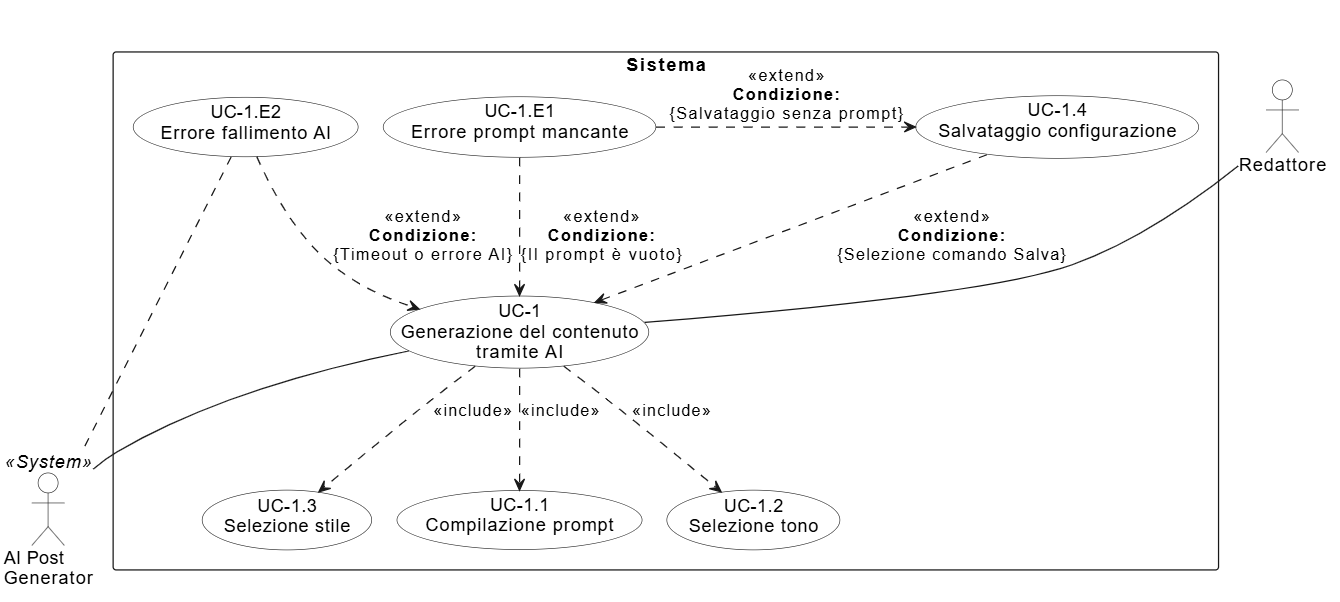
\includegraphics[width=1\textwidth]{diagrammi_use_case/UC-1.png}
    \caption{Diagramma del caso d'uso UC-1: Generazione del contenuto tramite AI}
    \label{fig:uc-1}
\end{figure}
\begin{description}[style=multiline, leftmargin=4cm, font=\bfseries]
    
    \item[\glslink{attore}{Attore} Principale] \glslink{redattore}{Redattore}
    
    \item[\glslink{attore-secondario}{Attore Secondario}] \glslink{ai-post-generator}{AI Post Generator}
    
    \item[\glslink{trigger}{Trigger}] Il \glslink{redattore}{Redattore} seleziona la funzione di creazione di un nuovo contenuto supportato dall'\glslink{intelligenza-artificiale-ai}{AI}.
    
    \item[Pre-condizioni]Il sistema ha inizializzato e reso operativo il modulo "\glslink{ai-assistant-generativo}{AI Assistant Generativo}", preimpostando i parametri di tono, stile e lunghezza sui valori di default.

    \item[Post-condizioni] Il sistema mostra l'anteprima del contenuto generato (comprendente titolo, testo e immagine di copertina) e abilita le funzionalità di revisione.
    
    \item[\glslink{scenario-principale}{Scenario Principale}]
    \begin{enumerate}[leftmargin=*, nosep]
        \item Il \glslink{redattore}{Redattore} accede all'interfaccia dell'\glslink{ai-assistant-generativo}{AI Assistant Generativo}, dove il sistema rende visibile l'area di lavoro.
        \item Il \glslink{redattore}{Redattore} compila il campo relativo al \glslink{prompt}{prompt} testuale (\textbf{UC-1.1}).
        \item Il \glslink{redattore}{Redattore} imposta il tono desiderato (\textbf{UC-1.2}).
        \item Il \glslink{redattore}{Redattore} imposta lo \glslink{stile-editoriale}{stile editoriale} (\textbf{UC-1.3}).
        \item Il \glslink{redattore}{Redattore} seleziona la lunghezza desiderata per la \glslink{bozza-draft}{bozza} (\textbf{UC-1.6}).
        \item Il \glslink{redattore}{Redattore} conferma l'avvio della generazione cliccando sul comando "Genera \glslink{bozza-draft}{bozza}".
        \item Il sistema visualizza a schermo l'anteprima del contenuto generato, comprendente titolo, testo e immagine di copertina (\textbf{UC-2}).
    \end{enumerate}
    \item[Scenari Alternativi]
     \begin{itemize}[leftmargin=*, nosep]
         \item \textbf{1a. Il \glslink{redattore}{Redattore} decide di svuotare i campi prima di iniziare}: viene eseguito \textbf{UC-1.5}.
         \item \textbf{5a. Il \glslink{redattore}{Redattore} decide di salvare la configurazione inserita}: viene eseguito \textbf{UC-1.4}.
         \item \textbf{6a. \glslink{prompt}{Prompt} mancante o insufficiente}: Il sistema rileva che il campo \glslink{prompt}{prompt} è vuoto o il testo non è sufficiente; viene eseguito \textbf{UC-1.E1}.
         \item \textbf{6b. Fallimento modulo \glslink{intelligenza-artificiale-ai}{AI}}: Il sistema rileva un errore di \glslink{timeout}{timeout} o di rete dal motore di generazione; viene eseguito \textbf{UC-1.E2}.
    \end{itemize}

    \item[Relazioni]
     \begin{itemize}[leftmargin=*, nosep]
         \item \textbf{Inclusioni}: UC-1.1, UC-1.2, UC-1.3, UC-1.6.
         \item \textbf{Estensioni}: UC-1.4, UC-1.5, UC-1.E1, UC-1.E2.
     \end{itemize}

\end{description}

\paragraph{UC-1.1: Compilazione del prompt descrittivo}
\mbox{}
\begin{figure}[H]
    \centering
    
\includegraphics[width=0.6\textwidth]{diagrammi_use_case/UC-1.1.png}
    \caption{Diagramma del caso d'uso UC-1.1: Compilazione del prompt descrittivo}
    \label{fig:uc-1.1}
\end{figure}
\begin{description}[style=multiline, leftmargin=4cm, font=\bfseries]
    \item[\glslink{attore}{Attore} Principale] \glslink{redattore}{Redattore}
    \item[Pre-condizioni] Il sistema è in attesa dei dati di input testuali.
    \item[Post-condizioni] Il testo del \glslink{prompt}{prompt} è stato registrato ed è pronto per l'elaborazione.
    \item[\glslink{scenario-principale}{Scenario Principale}] 
    \begin{enumerate}[leftmargin=*, nosep]
        \item Il \glslink{redattore}{Redattore} seleziona l'apposito campo di testo e vi inserisce la descrizione del contenuto desiderato.
    \end{enumerate}
\end{description}

\paragraph{UC-1.2: Selezione del tono comunicativo}
\mbox{}
\begin{figure}[H]
    \centering
    
\includegraphics[width=0.6\textwidth]{diagrammi_use_case/UC-1.2.png}
    \caption{Diagramma del caso d'uso UC-1.2: Selezione del tono comunicativo}
    \label{fig:uc-1.2}
\end{figure}
\begin{description}[style=multiline, leftmargin=4cm, font=\bfseries]
    \item[\glslink{attore}{Attore} Principale] \glslink{redattore}{Redattore}
    \item[Pre-condizioni] Il sistema espone l'elenco dei toni utilizzabili, impostato sul valore di default.
    \item[Post-condizioni] Il parametro relativo al tono di voce è stato impostato.
    \item[\glslink{scenario-principale}{Scenario Principale}] 
    \begin{enumerate}[leftmargin=*, nosep]
        \item Il \glslink{redattore}{Redattore} sceglie il tono del messaggio tramite il relativo menu a tendina.
    \end{enumerate}
\end{description}

\paragraph{UC-1.3: Selezione dello stile editoriale}
\mbox{}
\begin{figure}[H]
    \centering
    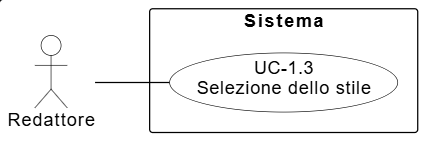
\includegraphics[width=0.6\textwidth]{diagrammi_use_case/UC-1.3.png}
    \caption{Diagramma del caso d'uso UC-1.3: Selezione dello stile editoriale}
    \label{fig:uc-1.3}
\end{figure}
\begin{description}[style=multiline, leftmargin=4cm, font=\bfseries]
    \item[\glslink{attore}{Attore} Principale] \glslink{redattore}{Redattore}
    \item[Pre-condizioni] Il sistema espone l'elenco degli stili di scrittura supportati, impostato sul valore di default.
    \item[Post-condizioni] Il parametro relativo allo stile è stato impostato.
    \item[\glslink{scenario-principale}{Scenario Principale}] 
    \begin{enumerate}[leftmargin=*, nosep]
        \item Il \glslink{redattore}{Redattore} indica lo stile desiderato tramite l'apposito menu di scelta.
    \end{enumerate}
\end{description}

\paragraph{UC-1.4: Salvataggio della configurazione del prompt}
\mbox{} \\
\begin{figure}[H]
    \centering
    
\includegraphics[width=0.9\textwidth]{diagrammi_use_case/UC-1.4.png}
    \caption{Diagramma del caso d'uso UC-1.4: Salvataggio della configurazione del prompt}
    \label{fig:uc-1.4}
\end{figure}
\begin{description}[style=multiline, leftmargin=4cm, font=\bfseries]
    \item[\glslink{attore}{Attore} Principale] \glslink{redattore}{Redattore}
    \item[Pre-condizioni] Il \glslink{redattore}{Redattore} ha compilato uno o più parametri nell'interfaccia di composizione.
    \item[Post-condizioni] La configurazione attuale è memorizzata nella libreria personale dei \glslink{prompt}{prompt} con un nome univoco.
    \item[\glslink{scenario-principale}{Scenario Principale}] 
    \begin{enumerate}[leftmargin=*, nosep]
        \item Il \glslink{redattore}{Redattore} seleziona il comando "Salva \glslink{prompt}{prompt}".
        \item Il sistema richiede l'inserimento di un nome identificativo per la configurazione.
        \item Il \glslink{redattore}{Redattore} conferma l'operazione (inserendo un nome oppure lasciando il campo vuoto).
        \item Il sistema elabora il nome: in caso di campo vuoto o di nome già esistente in libreria, il sistema assegna un'etichetta progressiva automatica (es. "Senza nome (1)").
        \item Il sistema memorizza i dati inseriti per consentirne il riutilizzo in sessioni successive.
    \end{enumerate}
    \item[Scenari Alternativi] 
    \begin{itemize}[leftmargin=*, nosep]
        \item \textbf{1a. \glslink{prompt}{Prompt} mancante}: Il \glslink{redattore}{Redattore} tenta il salvataggio con il campo \glslink{prompt}{prompt} principale vuoto; viene eseguito \textbf{UC-1.E1}.
    \end{itemize}

    \item[Relazioni] 
    \begin{itemize}[leftmargin=*, nosep]
        \item \textbf{Estensioni}: UC-1.E1.
    \end{itemize}
\end{description}

\paragraph{UC-1.5: Svuotamento dei campi di configurazione}
\mbox{} \\
\begin{figure}[H]
    \centering
    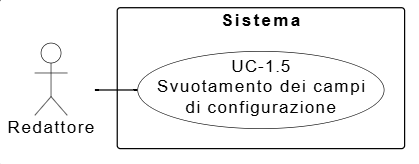
\includegraphics[width=0.5\textwidth]{diagrammi_use_case/UC-1.5.png}
    \caption{Diagramma del caso d'uso UC-1.5: Svuotamento dei campi di configurazione}
    \label{fig:uc-1.5}
\end{figure}
\begin{description}[style=multiline, leftmargin=4.5cm, font=\bfseries]
    \item[\glslink{attore}{Attore} Principale] \glslink{redattore}{Redattore}
    \item[Pre-condizioni] Il \glslink{redattore}{Redattore} ha compilato parzialmente o totalmente i campi di configurazione.
    \item[Post-condizioni] Il sistema ha ripristinato tutti i campi \glslink{intelligenza-artificiale-ai}{ai} valori predefiniti o vuoti.
    \item[\glslink{scenario-principale}{Scenario Principale}] 
    \begin{enumerate}[leftmargin=*, nosep]
        \item Il \glslink{redattore}{Redattore} seleziona il comando rapido di azzeramento (es. "Svuota campi").
        \item Il sistema cancella il testo inserito nel \glslink{prompt}{prompt} e ripristina le selezioni di tono e stile \glslink{intelligenza-artificiale-ai}{ai} valori di default.
    \end{enumerate}
\end{description}

\paragraph{UC-1.6: Selezione della lunghezza della bozza}
\mbox{} \\
\begin{figure}[H]
    \centering
    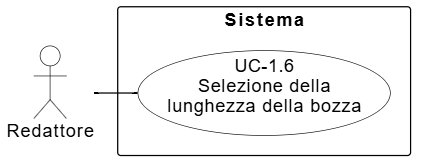
\includegraphics[width=0.6\textwidth]{diagrammi_use_case/UC-1.6.png}
    \caption{Diagramma del caso d'uso UC-1.6: Selezione della lunghezza della bozza}
    \label{fig:uc-1.6}
\end{figure}
\begin{description}[style=multiline, leftmargin=4.5cm, font=\bfseries]
    \item[\glslink{attore}{Attore} Principale] \glslink{redattore}{Redattore}
    \item[Pre-condizioni] Il sistema espone le opzioni di configurazione della lunghezza, impostate sul valore di default.
    \item[Post-condizioni] Il parametro relativo alla lunghezza del testo è stato impostato.
    \item[\glslink{scenario-principale}{Scenario Principale}] 
    \begin{enumerate}[leftmargin=*, nosep]
        \item Il \glslink{redattore}{Redattore} seleziona la lunghezza desiderata (es. breve, media, lunga) tramite l'apposito menu di scelta.
    \end{enumerate}
\end{description}


\paragraph{UC-1.E1: Errore - Prompt mancante o insufficiente}
\mbox{}
\begin{figure}[H]
    \centering
    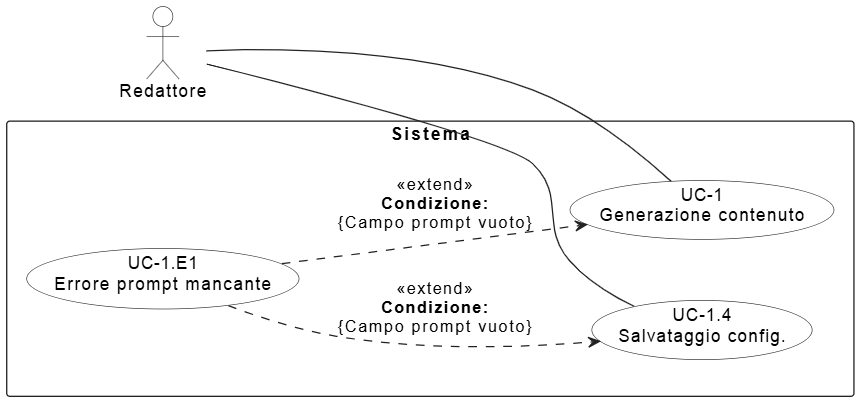
\includegraphics[width=0.6\textwidth]{diagrammi_use_case/UC-1.E1.png}
    \caption{Diagramma del caso d'uso UC-1.E1: Errore per prompt mancante o insufficiente}
    \label{fig:uc-1.e1}
\end{figure}
\begin{description}[style=multiline, leftmargin=4cm, font=\bfseries]
    \item[\glslink{attore}{Attore} Principale] \glslink{redattore}{Redattore}
    \item[Pre-condizioni] Il \glslink{redattore}{Redattore} tenta di avviare la generazione o il salvataggio con il campo \glslink{prompt}{prompt} vuoto.
    \item[Post-condizioni] Il sistema segnala l'errore e interrompe l'operazione di generazione.
    \item[\glslink{scenario-principale}{Scenario Principale}] 
    \begin{enumerate}[leftmargin=*, nosep]
        \item Il sistema rileva che l'input testuale è assente.
        \item Il sistema inibisce l'invio della richiesta e visualizza un messaggio di avviso.
    \end{enumerate}
\end{description}

\paragraph{UC-1.E2: Errore - Fallimento modulo AI}
\mbox{}
\begin{figure}[H]
    \centering
    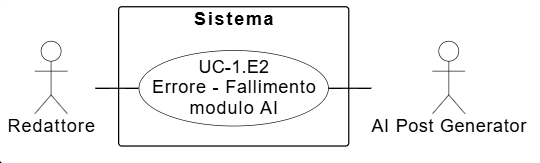
\includegraphics[width=0.7\textwidth]{diagrammi_use_case/UC-1.E2.png}
    \caption{Diagramma del caso d'uso UC-1.E2: Errore per fallimento del modulo AI}
    \label{fig:uc-1.e2}
\end{figure}
\begin{description}[style=multiline, leftmargin=4cm, font=\bfseries]
    \item[\glslink{attore}{Attore} Principale] \glslink{redattore}{Redattore}, \glslink{ai-post-generator}{AI Post Generator}
    \item[Pre-condizioni] Il sistema ha inviato i parametri al motore \glslink{intelligenza-artificiale-ai}{AI}, ma si verifica un \glslink{timeout}{timeout} o un errore di connessione.
    \item[Post-condizioni] Il sistema notifica il fallimento e mantiene i dati inseriti nell'interfaccia.
    \item[\glslink{scenario-principale}{Scenario Principale}] 
    \begin{enumerate}[leftmargin=*, nosep]
        \item Il sistema rileva l'impossibilità di completare la generazione.
        \item Il sistema mostra un messaggio di errore tecnico invitando l'utente a riprovare.
    \end{enumerate}
\end{description}
\newpage
\subsubsection{UC-2: Anteprima e revisione della bozza}

\mbox{} \\
\begin{figure}[H]
    \centering
    
\includegraphics[width=0.9\textwidth]{diagrammi_use_case/UC-2.png}
    \caption{Diagramma del caso d'uso UC-2: Anteprima e revisione della bozza}
    \label{fig:uc-2}
\end{figure}
\begin{description}[style=multiline, leftmargin=4cm, font=\bfseries]    
    \item[\glslink{attore}{Attore} Principale] \glslink{redattore}{Redattore}
    \item[\glslink{attore-secondario}{Attore Secondario}] \glslink{ai-post-generator}{AI Post Generator}
    
    \item[\glslink{trigger}{Trigger}] Il \glslink{redattore}{Redattore} analizza la \glslink{bozza-draft}{bozza} appena generata per controllarne la qualità ed eventualmente apportare modifiche.
    
    \item[Pre-condizioni] Il sistema ha completato la generazione (UC-1) e mostra l'anteprima della \glslink{bozza-draft}{bozza} (titolo, testo e immagine) nell'area di revisione.
    
    \item[Post-condizioni] Il sistema ha aggiornato la \glslink{bozza-draft}{bozza} in base alle scelte del \glslink{redattore}{Redattore}, rendendola pronta per l'approvazione e la finalizzazione (UC-3), oppure ha rimosso la \glslink{bozza-draft}{bozza} corrente.
    
    \item[\glslink{scenario-principale}{Scenario Principale}] 
    \begin{enumerate}[leftmargin=*, nosep]
        \item Il \glslink{redattore}{Redattore} visualizza l'anteprima del titolo della \glslink{bozza-draft}{bozza} (\textbf{UC-2.1}).
        \item Il \glslink{redattore}{Redattore} visualizza l'anteprima del testo della \glslink{bozza-draft}{bozza} (\textbf{UC-2.2}).
        \item Il \glslink{redattore}{Redattore} visualizza l'anteprima dell'immagine della \glslink{bozza-draft}{bozza} (\textbf{UC-2.3}).
        \item Il \glslink{redattore}{Redattore} modifica manualmente il titolo (\textbf{UC-2.4}).
        \item Il \glslink{redattore}{Redattore} modifica manualmente il testo (\textbf{UC-2.5}).
        \item Il \glslink{redattore}{Redattore} sostituisce l'immagine di copertina suggerita con un file locale (\textbf{UC-2.6}).
        \item Il \glslink{redattore}{Redattore} richiede la rigenerazione totale della \glslink{bozza-draft}{bozza} all'\glslink{intelligenza-artificiale-ai}{AI} (\textbf{UC-2.7}).
        \item Il \glslink{redattore}{Redattore} scarta la \glslink{bozza-draft}{bozza} corrente (\textbf{UC-2.8}).
        \item Il \glslink{redattore}{Redattore} annulla le modifiche manuali per ripristinare la \glslink{bozza-draft}{bozza} originale (\textbf{UC-2.9}).
    \end{enumerate}

    \item[Relazioni] 
    \begin{itemize}[leftmargin=*, nosep]
        \item \textbf{Inclusioni}: UC-2.1, UC-2.2, UC-2.3, UC-2.4, UC-2.5, UC-2.6, UC-2.7, UC-2.8, UC-2.9.
    \end{itemize}

\end{description}

\paragraph{UC-2.1: Visualizzazione del titolo generato}

\mbox{} \\

\begin{figure}[H]
    \centering
    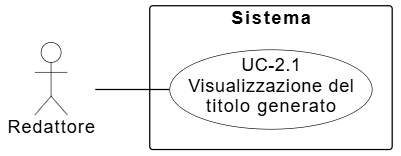
\includegraphics[width=0.6\textwidth]{diagrammi_use_case/UC-2.1.png}
    \caption{Diagramma del caso d'uso UC-2.1: Visualizzazione del titolo generato}
    \label{fig:uc-2.1}
\end{figure}
\begin{description}[style=multiline, leftmargin=4cm, font=\bfseries]
    \item[\glslink{attore}{Attore} Principale] \glslink{redattore}{Redattore}
    \item[Pre-condizioni] Il sistema ha predisposto la \glslink{bozza-draft}{bozza} generata.
    \item[Post-condizioni] Il \glslink{redattore}{Redattore} ha visualizzato il titolo suggerito.
    \item[\glslink{scenario-principale}{Scenario Principale}] 
    \begin{enumerate}[leftmargin=*, nosep]
        \item Il sistema espone a schermo il titolo elaborato all'interno dell'apposito campo testuale.
    \end{enumerate}
\end{description}

\paragraph{UC-2.2: Visualizzazione del testo generato}

\mbox{} \\

\begin{figure}[H]
    \centering
    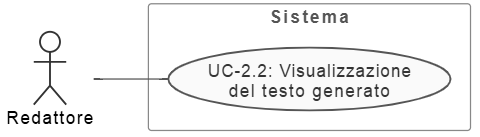
\includegraphics[width=0.6\textwidth]{diagrammi_use_case/UC-2.2.png}
    \caption{Diagramma del caso d'uso UC-2.2: Visualizzazione del testo generato}
    \label{fig:uc-2.2}
\end{figure}
\begin{description}[style=multiline, leftmargin=4cm, font=\bfseries]
    \item[\glslink{attore}{Attore} Principale] \glslink{redattore}{Redattore}
    \item[Pre-condizioni] Il sistema ha predisposto la \glslink{bozza-draft}{bozza} generata.
    \item[Post-condizioni] Il \glslink{redattore}{Redattore} ha visualizzato il corpo del testo suggerito.
    \item[\glslink{scenario-principale}{Scenario Principale}] 
    \begin{enumerate}[leftmargin=*, nosep]
        \item Il sistema presenta il testo della \glslink{bozza-draft}{bozza} all'interno dell'interfaccia di editing.
    \end{enumerate}
\end{description}

\paragraph{UC-2.3: Visualizzazione dell'immagine di copertina}
\mbox{} \\

\begin{figure}[H]
    \centering
    
\includegraphics[width=0.6\textwidth]{diagrammi_use_case/UC-2.3.png}
    \caption{Diagramma del caso d'uso UC-2.3: Visualizzazione dell'immagine di copertina}
    \label{fig:uc-2.3}
\end{figure}
\begin{description}[style=multiline, leftmargin=4cm, font=\bfseries]
    \item[\glslink{attore}{Attore} Principale] \glslink{redattore}{Redattore}
    \item[Pre-condizioni] Il sistema ha predisposto la \glslink{bozza-draft}{bozza} generata.
    \item[Post-condizioni] Il \glslink{redattore}{Redattore} ha visualizzato l'immagine suggerita.
    \item[\glslink{scenario-principale}{Scenario Principale}] 
    \begin{enumerate}[leftmargin=*, nosep]
        \item Il sistema visualizza l'anteprima grafica dell'immagine di copertina della \glslink{bozza-draft}{bozza}.
    \end{enumerate}
\end{description}

\paragraph{UC-2.4: Modifica manuale del titolo}
\mbox{} \\

\begin{figure}[H]
    \centering
    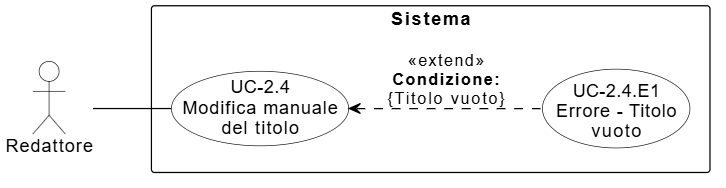
\includegraphics[width=0.8\textwidth]{diagrammi_use_case/UC-2.4.png}
    \caption{Diagramma del caso d'uso UC-2.4: Modifica manuale del titolo}
    \label{fig:uc-2.4}
\end{figure}
\begin{description}[style=multiline, leftmargin=4cm, font=\bfseries]
    \item[\glslink{attore}{Attore} Principale] \glslink{redattore}{Redattore}
    \item[Pre-condizioni] Il sistema presenta il titolo della \glslink{bozza-draft}{bozza} in un campo di testo interattivo.
    \item[Post-condizioni] Il sistema recepisce e visualizza le correzioni apportate al titolo della \glslink{bozza-draft}{bozza}.
    \item[\glslink{scenario-principale}{Scenario Principale}] 
    \begin{enumerate}[leftmargin=*, nosep]
        \item Il \glslink{redattore}{Redattore} seleziona il campo del titolo.
        \item Il \glslink{redattore}{Redattore} apporta le modifiche testuali.
        \item Il sistema aggiorna il titolo della \glslink{bozza-draft}{bozza}.
    \end{enumerate}
    \item[Scenari Alternativi] 
    \begin{itemize}[leftmargin=*, nosep]
        \item \textbf{3a. Titolo vuoto}: Il sistema rileva che il campo del titolo è stato completamente svuotato; viene eseguito \textbf{UC-2.E1}.
    \end{itemize}
    \item[Relazioni] 
    \begin{itemize}[leftmargin=*, nosep]
        \item \textbf{Estensioni}: UC-2.E1.
    \end{itemize}
\end{description}


\paragraph{UC-2.5: Modifica manuale del testo}
\mbox{} \\

\begin{figure}[H]
    \centering
    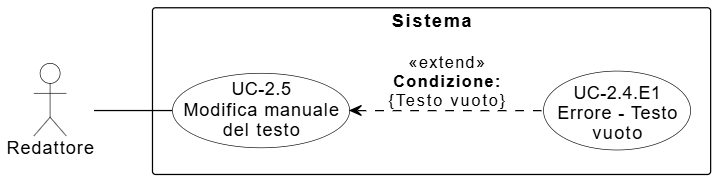
\includegraphics[width=0.8\textwidth]{diagrammi_use_case/UC-2.5.png}
    \caption{Diagramma del caso d'uso UC-2.5: Modifica manuale del testo}
    \label{fig:uc-2.5}
\end{figure}
\begin{description}[style=multiline, leftmargin=4cm, font=\bfseries]
    \item[\glslink{attore}{Attore} Principale] \glslink{redattore}{Redattore}
    \item[Pre-condizioni] Il sistema presenta il testo della \glslink{bozza-draft}{bozza} all'interno di un editor interattivo dotato di contatore.
    \item[Post-condizioni] Il sistema recepisce e visualizza le correzioni apportate al testo della \glslink{bozza-draft}{bozza}.
    \item[\glslink{scenario-principale}{Scenario Principale}] 
    \begin{enumerate}[leftmargin=*, nosep]
        \item Il \glslink{redattore}{Redattore} seleziona la porzione di testo da correggere.
        \item Il \glslink{redattore}{Redattore} digita le modifiche desiderate.
        \item Il sistema aggiorna l'anteprima a schermo.
    \end{enumerate}
    \item[Scenari Alternativi] 
    \begin{itemize}[leftmargin=*, nosep]
        \item \textbf{2a. Testo vuoto}: Il sistema rileva che il campo del testo è stato completamente svuotato; viene eseguito \textbf{UC-2.E1}.
    \end{itemize}
    \item[Relazioni] 
    \begin{itemize}[leftmargin=*, nosep]
        \item \textbf{Estensioni}: UC-2.E1.
    \end{itemize}
\end{description}

\paragraph{UC-2.6: Sostituzione dell'immagine di copertina}
\mbox{} \\

\begin{figure}[H]
    \centering
    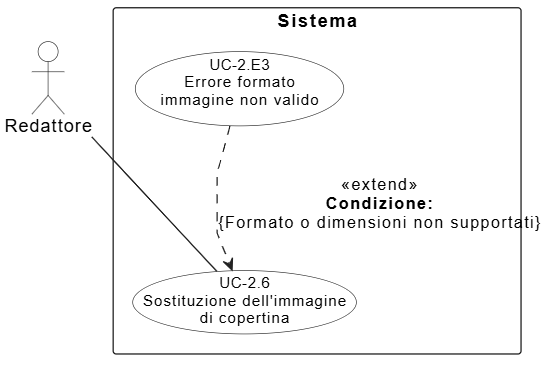
\includegraphics[width=0.9\textwidth]{diagrammi_use_case/UC-2.6.png}
    \caption{Diagramma del caso d'uso UC-2.6: Sostituzione dell'immagine di copertina}
    \label{fig:uc-2.6}
\end{figure}
\begin{description}[style=multiline, leftmargin=4cm, font=\bfseries]
    \item[\glslink{attore}{Attore} Principale] \glslink{redattore}{Redattore}
    \item[Pre-condizioni] Il sistema mostra l'anteprima dell'immagine suggerita nella \glslink{bozza-draft}{bozza}.
    \item[Post-condizioni] L'immagine di copertina della \glslink{bozza-draft}{bozza} è stata sostituita con un file scelto dal \glslink{redattore}{Redattore}.
    \item[\glslink{scenario-principale}{Scenario Principale}] 
    \begin{enumerate}[leftmargin=*, nosep]
        \item Il \glslink{redattore}{Redattore} seleziona l'opzione di modifica immagine.
        \item Il \glslink{redattore}{Redattore} carica un file immagine dal proprio dispositivo.
        \item Il sistema convalida il file e aggiorna l'anteprima grafica della \glslink{bozza-draft}{bozza}.
    \end{enumerate}
    \item[Scenari Alternativi] 
    \begin{itemize}[leftmargin=*, nosep]
        \item \textbf{2a. Formato immagine non valido}: Il sistema rileva che il file caricato non è supportato o supera i limiti di dimensione; viene eseguito \textbf{UC-2.6.E1}.
    \end{itemize}

    \item[Relazioni] 
    \begin{itemize}[leftmargin=*, nosep]
        \item \textbf{Estensioni}: UC-2.6.E1.
    \end{itemize}
\end{description}
\newpage
\paragraph{UC-2.7: Rigenerazione della bozza}
\mbox{} \\

\begin{figure}[H]
    \centering
    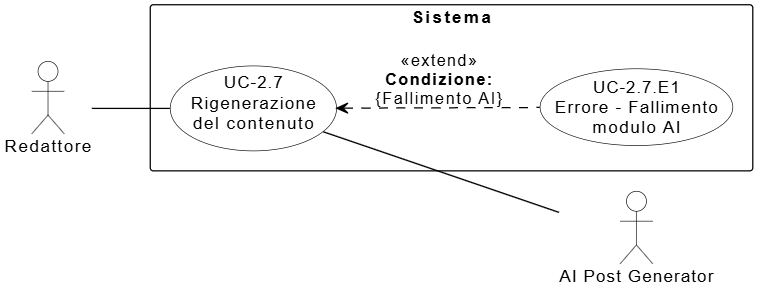
\includegraphics[width=0.8\textwidth]{diagrammi_use_case/UC-2.7.png}
    \caption{Diagramma del caso d'uso UC-2.7: Rigenerazione della bozza}
    \label{fig:uc-2.7}
\end{figure}
\begin{description}[style=multiline, leftmargin=4cm, font=\bfseries]
    \item[\glslink{attore}{Attore} Principale] \glslink{redattore}{Redattore}, \glslink{ai-post-generator}{AI Post Generator}
    \item[Pre-condizioni] Il sistema visualizza la \glslink{bozza-draft}{bozza} corrente e abilita il comando di rigenerazione.
    \item[Post-condizioni] Il sistema sostituisce la \glslink{bozza-draft}{bozza} precedente con una nuova variante elaborata.
    \item[\glslink{scenario-principale}{Scenario Principale}] 
    \begin{enumerate}[leftmargin=*, nosep]
        \item Il \glslink{redattore}{Redattore} richiede una nuova variante tramite l'apposito comando.
        \item Il sistema visualizza a schermo la nuova \glslink{bozza-draft}{bozza} generata.
    \end{enumerate}
    \item[Scenari Alternativi] 
    \begin{itemize}[leftmargin=*, nosep]
        \item \textbf{1a. Fallimento modulo \glslink{intelligenza-artificiale-ai}{AI}}: Il sistema rileva un errore di rete o di API durante la richiesta della variante; viene eseguito \textbf{UC-2.7.E1}.
    \end{itemize}

    \item[Relazioni] 
    \begin{itemize}[leftmargin=*, nosep]
        \item \textbf{Estensioni}: UC-2.7.E1.
    \end{itemize}
\end{description}

\paragraph{UC-2.8: Eliminazione della bozza generata}
\mbox{} \\

\begin{figure}[H]
    \centering
    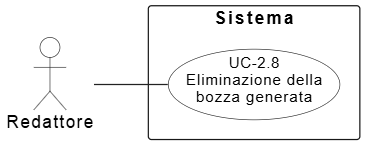
\includegraphics[width=0.5\textwidth]{diagrammi_use_case/UC-2.8.png}
    \caption{Diagramma del caso d'uso UC-2.8: Eliminazione della bozza generata}
    \label{fig:uc-2.8}
\end{figure}
\begin{description}[style=multiline, leftmargin=4cm, font=\bfseries]
    \item[\glslink{attore}{Attore} Principale] \glslink{redattore}{Redattore}
    \item[Pre-condizioni] Il sistema visualizza l'anteprima della \glslink{bozza-draft}{bozza} corrente.
    \item[Post-condizioni] Il sistema ha eliminato la \glslink{bozza-draft}{bozza} e svuotato l'area di lavoro.
    \item[\glslink{scenario-principale}{Scenario Principale}] 
    \begin{enumerate}[leftmargin=*, nosep]
        \item Il \glslink{redattore}{Redattore} seleziona il comando di eliminazione definitiva.
        \item Il sistema richiede una conferma per l'operazione.
        \item Il \glslink{redattore}{Redattore} conferma l'intenzione di scartare la \glslink{bozza-draft}{bozza}.
        \item Il sistema riporta l'utente alla schermata di configurazione iniziale.
    \end{enumerate}
\end{description}

\paragraph{UC-2.9: Annullamento delle modifiche manuali}
\mbox{} \\
\begin{figure}[H]
    \centering
    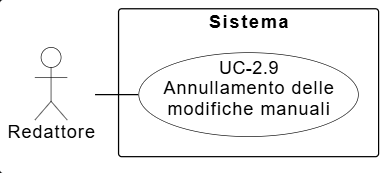
\includegraphics[width=0.5\textwidth]{diagrammi_use_case/UC-2.9.png}
    \caption{Diagramma del caso d'uso UC-2.9: Annullamento delle modifiche manuali}
    \label{fig:uc-2.9}
\end{figure}
\begin{description}[style=multiline, leftmargin=4.5cm, font=\bfseries]
    \item[\glslink{attore}{Attore} Principale] \glslink{redattore}{Redattore}
    \item[Pre-condizioni] Il \glslink{redattore}{Redattore} ha apportato modifiche manuali alla \glslink{bozza-draft}{bozza} (UC-2.4 o UC-2.5).
    \item[Post-condizioni] Il sistema ha ripristinato la \glslink{bozza-draft}{bozza} alla versione originariamente generata dall'\glslink{intelligenza-artificiale-ai}{AI}.
    \item[\glslink{scenario-principale}{Scenario Principale}] 
    \begin{enumerate}[leftmargin=*, nosep]
        \item Il \glslink{redattore}{Redattore} seleziona il comando "Annulla modifiche".
        \item Il sistema sovrascrive le modifiche manuali e ricarica a schermo la \glslink{bozza-draft}{bozza} originale elaborata dal modulo \glslink{intelligenza-artificiale-ai}{AI}.
    \end{enumerate}
\end{description}

\paragraph{UC-2.E1: Errore - Contenuto vuoto}
\mbox{} \\

\begin{figure}[H]
    \centering
    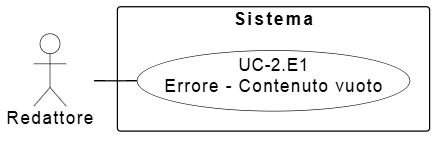
\includegraphics[width=0.6\textwidth]{diagrammi_use_case/UC-2.E1.png}
    \caption{Diagramma del caso d'uso UC-2.E1: Errore per contenuto vuoto}
    \label{fig:uc-2.e1}
\end{figure}
\begin{description}[style=multiline, leftmargin=4cm, font=\bfseries]
    \item[\glslink{attore}{Attore} Principale] \glslink{redattore}{Redattore}
    \item[Pre-condizioni] Il \glslink{redattore}{Redattore} ha svuotato un campo obbligatorio della \glslink{bozza-draft}{bozza} (titolo in UC-2.4 o testo in UC-2.5) e tenta di confermare le modifiche.
    \item[Post-condizioni] Il sistema non applica le modifiche, mantenendo l'ultima versione valida del campo.
    \item[\glslink{scenario-principale}{Scenario Principale}] 
    \begin{enumerate}[leftmargin=*, nosep]
        \item Il sistema rileva che il campo obbligatorio è stato completamente svuotato.
        \item Il sistema blocca l'aggiornamento e segnala visivamente l'obbligatorietà del campo.
        \item Il sistema ripristina l'ultima versione valida del campo.
    \end{enumerate}
\end{description}

\paragraph{UC-2.7.E1: Errore - Fallimento modulo AI}
\mbox{} \\

\begin{figure}[H]
    \centering
    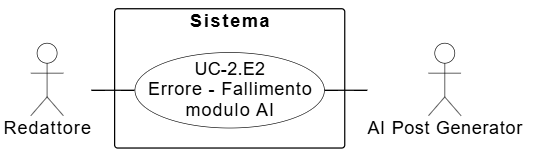
\includegraphics[width=0.7\textwidth]{diagrammi_use_case/UC-2.E2.png}
    \caption{Diagramma del caso d'uso UC-2.7.E1: Errore per fallimento modulo AI}
    \label{fig:uc-2.7.e1}
\end{figure}
\begin{description}[style=multiline, leftmargin=4cm, font=\bfseries]
    \item[\glslink{attore}{Attore} Principale] \glslink{redattore}{Redattore}, \glslink{ai-post-generator}{AI Post Generator}
    \item[Pre-condizioni] Il \glslink{redattore}{Redattore} ha richiesto la rigenerazione della \glslink{bozza-draft}{bozza}, ma si verifica un problema tecnico di rete o di API.
    \item[Post-condizioni] Il sistema notifica il fallimento e preserva l'ultima \glslink{bozza-draft}{bozza} valida a schermo.
    \item[\glslink{scenario-principale}{Scenario Principale}] 
    \begin{enumerate}[leftmargin=*, nosep]
        \item Il sistema rileva l'impossibilità di ottenere la nuova versione.
        \item Il sistema mostra un messaggio di errore tecnico e mantiene visibile la \glslink{bozza-draft}{bozza} su cui si stava lavorando.
    \end{enumerate}
\end{description}

\paragraph{UC-2.6.E1: Errore - Formato immagine non valido}
\mbox{} \\

\begin{figure}[H]
    \centering
    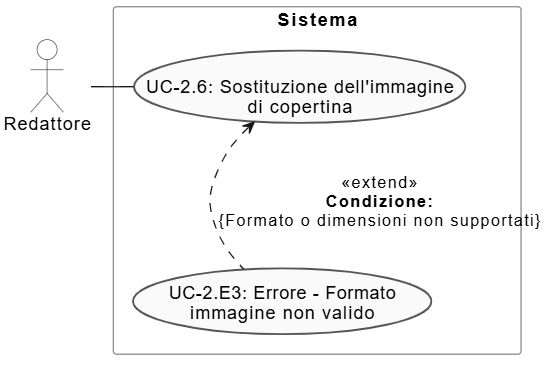
\includegraphics[width=0.5\textwidth]{diagrammi_use_case/UC-2.E3.png}
    \caption{Diagramma del caso d'uso UC-2.6.E1: Errore per formato immagine non valido}
    \label{fig:uc-2.6.e1}
\end{figure}
\begin{description}[style=multiline, leftmargin=4cm, font=\bfseries]
    \item[\glslink{attore}{Attore} Principale] \glslink{redattore}{Redattore}
    \item[Pre-condizioni] Il \glslink{redattore}{Redattore} tenta di caricare una nuova immagine che non rispetta i vincoli di sistema.
    \item[Post-condizioni] Il sistema impedisce il caricamento e mantiene l'immagine precedente nella \glslink{bozza-draft}{bozza}.
    \item[\glslink{scenario-principale}{Scenario Principale}] 
    \begin{enumerate}[leftmargin=*, nosep]
        \item Il sistema rileva che il file non è supportato o supera la dimensione massima consentita.
        \item Il sistema visualizza un messaggio di errore e richiede l'inserimento di un file valido.
    \end{enumerate}
\end{description}

\subsubsection{UC-3: Approvazione e finalizzazione del documento}
\mbox{} \\
\begin{figure}[H]
    \centering
    
\includegraphics[width=1.1\textwidth]{diagrammi_use_case/UC-3.png}
    \caption{Diagramma del caso d'uso UC-3: Approvazione e finalizzazione del documento}
    \label{fig:uc-3}
\end{figure}
\begin{description}[style=multiline, leftmargin=4cm, font=\bfseries]
    
    \item[\glslink{attore}{Attore} Principale] \glslink{redattore}{Redattore}
    
    \item[\glslink{trigger}{Trigger}] Il \glslink{redattore}{Redattore} ha concluso la fase di revisione della \glslink{bozza-draft}{bozza} e intende approvarla e finalizzarla in un documento da archiviare, esportare o distribuire.

    \item[Pre-condizioni] La \glslink{bozza-draft}{bozza} revisionata (UC-2) è pronta per l'approvazione.
    
    \item[Post-condizioni] Il sistema ha promosso la \glslink{bozza-draft}{bozza} a documento e lo ha archiviato, esportato o inoltrato con successo; nei casi di esportazione e inoltro il documento riporta in calce il \glslink{marcatore-di-trasparenza}{marcatore di trasparenza} ``Creato da \glslink{intelligenza-artificiale-ai}{AI} Assistant''.
    
    \item[\glslink{scenario-principale}{Scenario Principale}] 
    \begin{enumerate}[leftmargin=*, nosep]
        \item Il \glslink{redattore}{Redattore} visualizza le opzioni di finalizzazione disponibili (\textbf{UC-3.1}).
        \item Il \glslink{redattore}{Redattore} visualizza l'anteprima del documento finale (\textbf{UC-3.5}).
        \item Il \glslink{redattore}{Redattore} archivia il documento selezionando il salvataggio in \glslink{bozza-draft}{bozza} (\textbf{UC-3.2}).
        \item Il \glslink{redattore}{Redattore} scarica il documento selezionando il comando di esportazione (\textbf{UC-3.3}).
        \item Il \glslink{redattore}{Redattore} distribuisce il documento selezionando l'inoltro tramite posta elettronica (\textbf{UC-3.4}).
    \end{enumerate}

    \item[Relazioni] 
    \begin{itemize}[leftmargin=*, nosep]
        \item \textbf{Inclusioni}: UC-3.1, UC-3.2, UC-3.3, UC-3.4, UC-3.5.
    \end{itemize}

\end{description}

\paragraph{UC-3.1: Visualizzazione delle opzioni di finalizzazione}
\mbox{} \\

\begin{figure}[H]
    \centering
    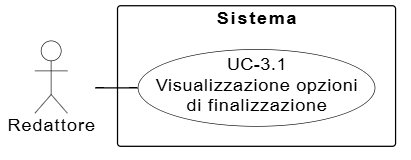
\includegraphics[width=0.5\textwidth]{diagrammi_use_case/UC-3.1.png}
    \caption{Diagramma del caso d'uso UC-3.1: Visualizzazione delle opzioni di finalizzazione}
    \label{fig:uc-3.1}
\end{figure}
\begin{description}[style=multiline, leftmargin=4cm, font=\bfseries]
    \item[\glslink{attore}{Attore} Principale] \glslink{redattore}{Redattore}
    \item[Pre-condizioni] Il sistema ha validato l'ultima versione della \glslink{bozza-draft}{bozza} al termine della fase di revisione.
    \item[Post-condizioni] Il sistema espone i comandi di gestione finale del documento.
    \item[\glslink{scenario-principale}{Scenario Principale}] 
    \begin{enumerate}[leftmargin=*, nosep]
        \item Il sistema rende visibili i comandi per il salvataggio in \glslink{bozza-draft}{bozza}, l'esportazione locale e l'invio telematico.
    \end{enumerate}
\end{description}
\newpage
\paragraph{UC-3.2: Salvataggio in bozza}
\mbox{} \\

\begin{figure}[H]
    \centering
    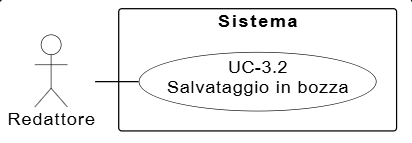
\includegraphics[width=0.5\textwidth]{diagrammi_use_case/UC-3.2.png}
    \caption{Diagramma del caso d'uso UC-3.2: Salvataggio in bozza}
    \label{fig:uc-3.2}
\end{figure}
\begin{description}[style=multiline, leftmargin=4cm, font=\bfseries]
    \item[\glslink{attore}{Attore} Principale] \glslink{redattore}{Redattore}
    \item[Pre-condizioni] Il sistema mostra i comandi di finalizzazione.
    \item[Post-condizioni] Il sistema ha memorizzato lo stato attuale del documento nell'area personale del \glslink{redattore}{Redattore}, conservandolo come \glslink{bozza-draft}{bozza} riprendibile.
    \item[\glslink{scenario-principale}{Scenario Principale}] 
    \begin{enumerate}[leftmargin=*, nosep]
        \item Il \glslink{redattore}{Redattore} seleziona l'opzione di salvataggio in \glslink{bozza-draft}{bozza}.
        \item Il sistema conferma a video l'avvenuta archiviazione.
    \end{enumerate}
\end{description}

\paragraph{UC-3.3: Esportazione del documento in PDF}
\mbox{} \\
\begin{figure}[H]
    \centering
    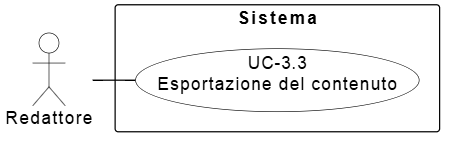
\includegraphics[width=0.5\textwidth]{diagrammi_use_case/UC-3.3.png}
    \caption{Diagramma del caso d'uso UC-3.3: Esportazione del documento}
    \label{fig:uc-3.3}
\end{figure}
\begin{description}[style=multiline, leftmargin=4.5cm, font=\bfseries]
    \item[\glslink{attore}{Attore} Principale] \glslink{redattore}{Redattore}
    \item[Pre-condizioni] Il sistema mostra i comandi di finalizzazione.
    \item[Post-condizioni] Il sistema ha generato un file PDF scaricabile comprensivo del \glslink{marcatore-di-trasparenza}{marcatore di trasparenza} ``Creato da \glslink{intelligenza-artificiale-ai}{AI} Assistant''.
    \item[\glslink{scenario-principale}{Scenario Principale}] 
    \begin{enumerate}[leftmargin=*, nosep]
        \item Il \glslink{redattore}{Redattore} seleziona il comando di esportazione PDF.
        \item Il sistema avvia il download del documento sul dispositivo dell'utente nel formato PDF.
    \end{enumerate}
\end{description}

\paragraph{UC-3.4: Inoltro tramite e-mail}
\mbox{} \\

\begin{figure}[H]
    \centering
    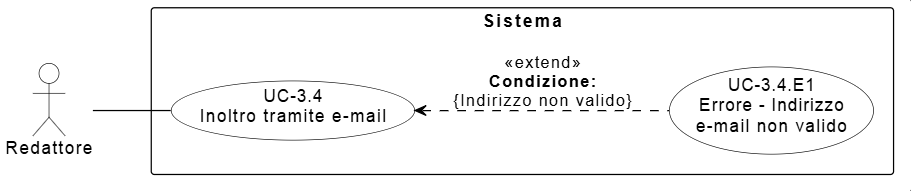
\includegraphics[width=0.9\textwidth]{diagrammi_use_case/UC-3.4.png}
    \caption{Diagramma del caso d'uso UC-3.4: Inoltro tramite e-mail}
    \label{fig:uc-3.4}
\end{figure}
\begin{description}[style=multiline, leftmargin=4cm, font=\bfseries]
    \item[\glslink{attore}{Attore} Principale] \glslink{redattore}{Redattore}
    \item[Pre-condizioni] Il sistema espone il campo per l'inserimento dell'indirizzo del destinatario.
    \item[Post-condizioni] Il documento è stato trasmesso con successo all'indirizzo specificato, con il \glslink{marcatore-di-trasparenza}{marcatore di trasparenza} ``Creato da \glslink{intelligenza-artificiale-ai}{AI} Assistant''.
    \item[\glslink{scenario-principale}{Scenario Principale}] 
    \begin{enumerate}[leftmargin=*, nosep]
        \item Il \glslink{redattore}{Redattore} seleziona l'opzione di invio e inserisce l'indirizzo e-mail di destinazione.
        \item Il sistema trasmette il messaggio includendo il \glslink{marcatore-di-trasparenza}{marcatore di trasparenza}.
        \item Il sistema notifica il successo dell'operazione.
    \end{enumerate}
    \item[Scenari Alternativi] 
    \begin{itemize}[leftmargin=*, nosep]
        \item \textbf{1a. Indirizzo e-mail non valido}: Il sistema rileva che l'indirizzo inserito per l'inoltro non rispetta il formato standard; viene eseguito \textbf{UC-3.4.E1}.
    \end{itemize}

    \item[Relazioni] 
    \begin{itemize}[leftmargin=*, nosep]
        \item \textbf{Estensioni}: UC-3.4.E1.
    \end{itemize}
\end{description}

\paragraph{UC-3.5: Visualizzazione anteprima di esportazione}
\mbox{} \\
\begin{figure}[H]
    \centering
    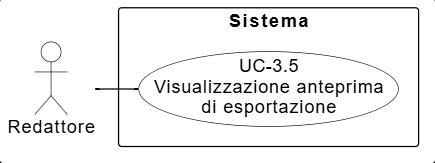
\includegraphics[width=0.5\textwidth]{diagrammi_use_case/UC-3.5.png}
    \caption{Diagramma del caso d'uso UC-3.5: Visualizzazione anteprima di esportazione}
    \label{fig:uc-3.5}
\end{figure}
\begin{description}[style=multiline, leftmargin=4.5cm, font=\bfseries]
    \item[\glslink{attore}{Attore} Principale] \glslink{redattore}{Redattore}
    \item[Pre-condizioni] Il sistema mostra i comandi di finalizzazione e il \glslink{redattore}{Redattore} intende esportare il documento.
    \item[Post-condizioni] Il \glslink{redattore}{Redattore} ha visualizzato a schermo l'aspetto del documento finale, comprensivo del \glslink{marcatore-di-trasparenza}{marcatore di trasparenza} ``Creato da \glslink{intelligenza-artificiale-ai}{AI} Assistant''.
    \item[\glslink{scenario-principale}{Scenario Principale}] 
    \begin{enumerate}[leftmargin=*, nosep]
        \item Il \glslink{redattore}{Redattore} seleziona il comando di anteprima di stampa/esportazione.
        \item Il sistema genera e mostra a schermo una preview del documento impaginato, rendendo visibile il \glslink{marcatore-di-trasparenza}{marcatore di trasparenza}.
    \end{enumerate}
\end{description}

\paragraph{UC-3.4.E1: Errore - Indirizzo e-mail non valido}
\mbox{} \\

\begin{figure}[H]
    \centering
    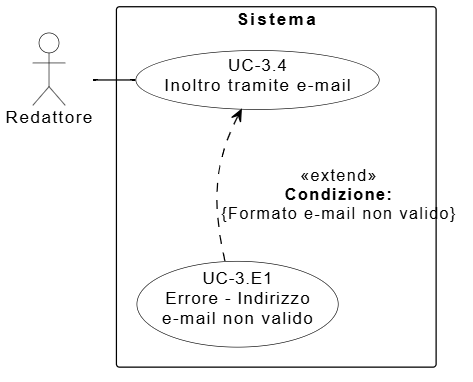
\includegraphics[width=0.5\textwidth]{diagrammi_use_case/UC-3.E1.png}
    \caption{Diagramma del caso d'uso UC-3.4.E1: Errore per indirizzo e-mail non valido}
    \label{fig:uc-3.4.e1}
\end{figure}
\begin{description}[style=multiline, leftmargin=4cm, font=\bfseries]
    \item[\glslink{attore}{Attore} Principale] \glslink{redattore}{Redattore}
    \item[Pre-condizioni] Il \glslink{redattore}{Redattore} richiede l'inoltro inserendo un indirizzo sintatticamente errato.
    \item[Post-condizioni] Il sistema blocca la procedura di invio e segnala l'anomalia.
    \item[\glslink{scenario-principale}{Scenario Principale}] 
    \begin{enumerate}[leftmargin=*, nosep]
        \item Il sistema intercetta il formato e-mail non valido.
        \item Il sistema evidenzia il campo errato e richiede l'inserimento di un indirizzo corretto.
    \end{enumerate}
\end{description}
\newpage
\subsubsection{UC-4: Gestione libreria prompt e storico}
\mbox{} \\

\begin{figure}[H]
    \centering
    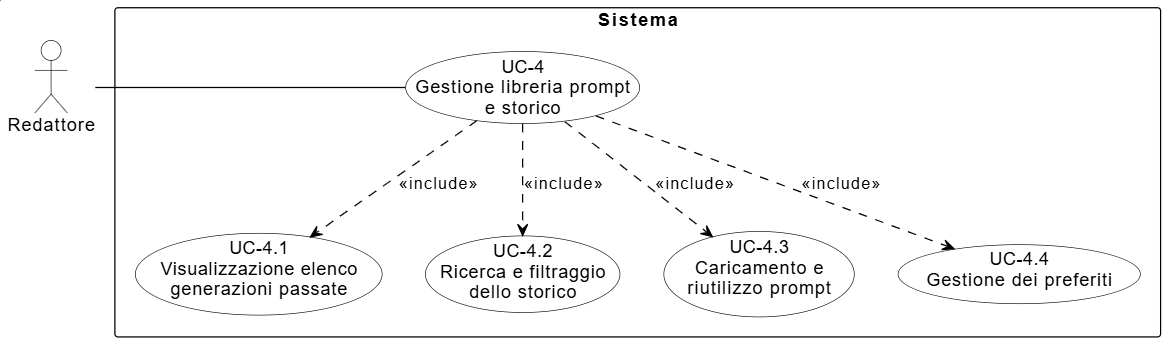
\includegraphics[width=1\textwidth]{diagrammi_use_case/UC-4.png}
    \caption{Diagramma del caso d'uso UC-4: Gestione libreria prompt e storico}
    \label{fig:uc-4}
\end{figure}
\begin{description}[style=multiline, leftmargin=4cm, font=\bfseries]
    
    \item[\glslink{attore}{Attore} Principale] \glslink{redattore}{Redattore}
    
    \item[\glslink{trigger}{Trigger}] Il \glslink{redattore}{Redattore} intende consultare, filtrare o riutilizzare le generazioni archiviate nelle sessioni precedenti.

    \item[Pre-condizioni] Il \glslink{redattore}{Redattore} accede alla sezione dedicata, che raccoglie cronologicamente le generazioni passate (storico) e ne consente il riuso come libreria di \glslink{prompt}{prompt}.
    
    \item[Post-condizioni] Il sistema ha permesso la consultazione, la ricerca o il riutilizzo delle generazioni archiviate.
    
    \item[\glslink{scenario-principale}{Scenario Principale}] 
    \begin{enumerate}[leftmargin=*, nosep]
        \item Il \glslink{redattore}{Redattore} visualizza l'elenco cronologico delle generazioni passate (\textbf{UC-4.1}).
        \item Il \glslink{redattore}{Redattore} effettua una ricerca o applica filtri allo storico (\textbf{UC-4.2}).
        \item Il \glslink{redattore}{Redattore} seleziona una generazione archiviata per riutilizzarne il \glslink{prompt}{prompt} (\textbf{UC-4.3}).
        \item Il \glslink{redattore}{Redattore} gestisce le generazioni preferite tramite \glslink{bookmark}{bookmark} (\textbf{UC-4.4}).
        \item Il \glslink{redattore}{Redattore} elimina un elemento dallo storico (\textbf{UC-4.5}).
    \end{enumerate}
    \item[Relazioni] 
    \begin{itemize}[leftmargin=*, nosep]
        \item \textbf{Inclusioni}: UC-4.1, UC-4.2, UC-4.3, UC-4.4, UC-4.5.
    \end{itemize}
\end{description}

\paragraph{UC-4.1: Visualizzazione elenco generazioni passate}
\mbox{} \\

\begin{figure}[H]
    \centering
    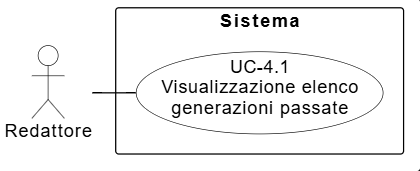
\includegraphics[width=0.5\textwidth]{diagrammi_use_case/UC-4.1.png}
    \caption{Diagramma del caso d'uso UC-4.1: Visualizzazione elenco generazioni passate}
    \label{fig:uc-4.1}
\end{figure}
\begin{description}[style=multiline, leftmargin=4cm, font=\bfseries]
    \item[\glslink{attore}{Attore} Principale] \glslink{redattore}{Redattore}
    \item[Pre-condizioni] Il \glslink{redattore}{Redattore} si trova nella sezione dedicata alla libreria.
    \item[Post-condizioni] Il sistema espone la lista dei \glslink{prompt}{prompt} e dei risultati precedentemente generati.
    \item[\glslink{scenario-principale}{Scenario Principale}] 
    \begin{enumerate}[leftmargin=*, nosep]
        \item Il sistema mostra l'elenco in ordine cronologico decrescente, includendo anteprima del \glslink{prompt}{prompt}, tono e data.
    \end{enumerate}
\end{description}

\paragraph{UC-4.2: Ricerca e filtraggio dello storico}
\mbox{} \\

\begin{figure}[H]
    \centering
    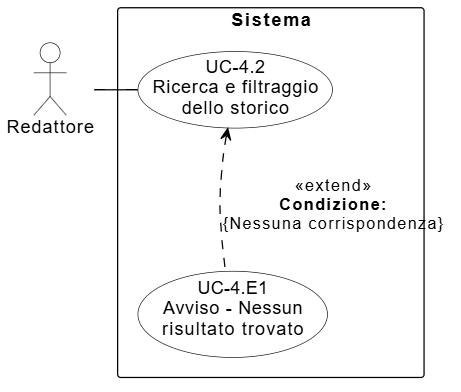
\includegraphics[width=0.9\textwidth]{diagrammi_use_case/UC-4.2.png}
    \caption{Diagramma del caso d'uso UC-4.2: Ricerca e filtraggio dello storico}
    \label{fig:uc-4.2}
\end{figure}
\begin{description}[style=multiline, leftmargin=4cm, font=\bfseries]
    \item[\glslink{attore}{Attore} Principale] \glslink{redattore}{Redattore}
    \item[Pre-condizioni] Il \glslink{redattore}{Redattore} visualizza l'elenco cronologico.
    \item[Post-condizioni] Il sistema aggiorna la lista in base \glslink{intelligenza-artificiale-ai}{ai} criteri inseriti.
    \item[\glslink{scenario-principale}{Scenario Principale}] 
    \begin{enumerate}[leftmargin=*, nosep]
        \item Il \glslink{redattore}{Redattore} inserisce una parola chiave nel campo di ricerca o seleziona un filtro (tono, stile o data).
        \item Il sistema aggiorna dinamicamente i contenuti visualizzati a schermo.
    \end{enumerate}
    \item[Scenari Alternativi] 
    \begin{itemize}[leftmargin=*, nosep]
        \item \textbf{2a. Nessun risultato trovato}: Il sistema rileva che i criteri di ricerca o i filtri applicati non producono alcuna corrispondenza; viene eseguito \textbf{UC-4.2.E1}.
    \end{itemize}

    \item[Relazioni] 
    \begin{itemize}[leftmargin=*, nosep]
        \item \textbf{Estensioni}: UC-4.2.E1.
    \end{itemize}
\end{description}

\paragraph{UC-4.3: Caricamento e riutilizzo prompt}
\mbox{} \\

\begin{figure}[H]
    \centering
    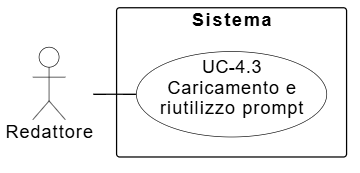
\includegraphics[width=0.45\textwidth]{diagrammi_use_case/UC-4.3.png}
    \caption{Diagramma del caso d'uso UC-4.3: Caricamento e riutilizzo prompt}
    \label{fig:uc-4.3}
\end{figure}
\begin{description}[style=multiline, leftmargin=4cm, font=\bfseries]
    \item[\glslink{attore}{Attore} Principale] \glslink{redattore}{Redattore}
    \item[Pre-condizioni] Il \glslink{redattore}{Redattore} ha individuato una generazione d'interesse nella libreria.
    \item[Post-condizioni] Il sistema predispone l'interfaccia di generazione con i parametri del \glslink{prompt}{prompt} selezionato.
    \item[\glslink{scenario-principale}{Scenario Principale}] 
    \begin{enumerate}[leftmargin=*, nosep]
        \item Il \glslink{redattore}{Redattore} seleziona il comando di riutilizzo su una generazione archiviata.
        \item Il sistema riporta l'utente alla schermata di configurazione (UC-1) pre-compilando automaticamente tutti i campi con i parametri del \glslink{prompt}{prompt} selezionato.
    \end{enumerate}
\end{description}

\paragraph{UC-4.4: Gestione dei preferiti}
\mbox{} \\

\begin{figure}[H]
    \centering
    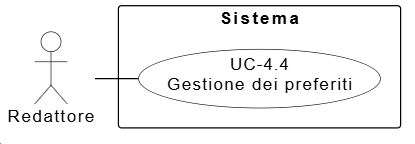
\includegraphics[width=0.5\textwidth]{diagrammi_use_case/UC-4.4.png}
    \caption{Diagramma del caso d'uso UC-4.4: Gestione dei preferiti}
    \label{fig:uc-4.4}
\end{figure}
\begin{description}[style=multiline, leftmargin=4cm, font=\bfseries]
    \item[\glslink{attore}{Attore} Principale] \glslink{redattore}{Redattore}
    \item[Pre-condizioni] Il \glslink{redattore}{Redattore} visualizza l'elenco delle generazioni archiviate nella libreria.
    \item[Post-condizioni] Il sistema aggiorna lo stato di preferenza della generazione selezionata.
    \item[\glslink{scenario-principale}{Scenario Principale}] 
    \begin{enumerate}[leftmargin=*, nosep]
        \item Il \glslink{redattore}{Redattore} seleziona l'icona dedicata per contrassegnare la generazione come preferita o per rimuovere la preferenza.
        \item Il sistema fornisce un feedback visivo immediato (cambio colore).
    \end{enumerate}
\end{description}

\paragraph{UC-4.5: Eliminazione di un elemento dallo storico}
\mbox{} \\

\begin{figure}[H]
    \centering
    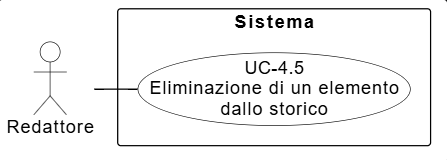
\includegraphics[width=0.6\textwidth]{diagrammi_use_case/UC-4.5.png}
    \caption{Diagramma del caso d'uso UC-4.5: Eliminazione di un elemento dallo storico}
    \label{fig:uc-4.5}
\end{figure}
\begin{description}[style=multiline, leftmargin=4.5cm, font=\bfseries]
    \item[\glslink{attore}{Attore} Principale] \glslink{redattore}{Redattore}
    \item[Pre-condizioni] Il \glslink{redattore}{Redattore} ha individuato un elemento nello storico che desidera rimuovere.
    \item[Post-condizioni] Il sistema ha rimosso definitivamente l'elemento selezionato dal database.
    \item[\glslink{scenario-principale}{Scenario Principale}] 
    \begin{enumerate}[leftmargin=*, nosep]
        \item Il \glslink{redattore}{Redattore} seleziona il comando di eliminazione in corrispondenza di un \glslink{prompt}{prompt} archiviato.
        \item Il sistema richiede una conferma di sicurezza per procedere.
        \item Il \glslink{redattore}{Redattore} conferma l'operazione.
        \item Il sistema rimuove l'elemento e aggiorna dinamicamente la lista a schermo.
    \end{enumerate}
\end{description}

\paragraph{UC-4.2.E1: Avviso - Nessun risultato trovato}
\mbox{} \\

\begin{figure}[H]
    \centering
    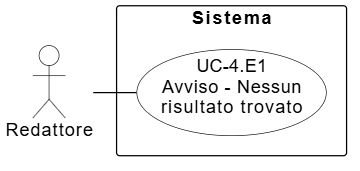
\includegraphics[width=0.5\textwidth]{diagrammi_use_case/UC-4.E1.png}
    \caption{Diagramma del caso d'uso UC-4.2.E1: Avviso per nessun risultato trovato}
    \label{fig:uc-4.2.e1}
\end{figure}
\begin{description}[style=multiline, leftmargin=4cm, font=\bfseries]
    \item[\glslink{attore}{Attore} Principale] \glslink{redattore}{Redattore}
    \item[Pre-condizioni] Il \glslink{redattore}{Redattore} ha inserito criteri di ricerca che non producono risultati.
    \item[Post-condizioni] Il sistema segnala l'assenza di elementi e permette di azzerare i criteri.
    \item[\glslink{scenario-principale}{Scenario Principale}] 
    \begin{enumerate}[leftmargin=*, nosep]
        \item Il sistema visualizza il messaggio "Nessun risultato trovato".
        \item Il sistema offre un comando rapido per rimuovere i filtri applicati.
    \end{enumerate}
\end{description}

\subsubsection{UC-5: Sistema di valutazione e feedback}
\mbox{} \\
\begin{figure}[H]
    \centering
    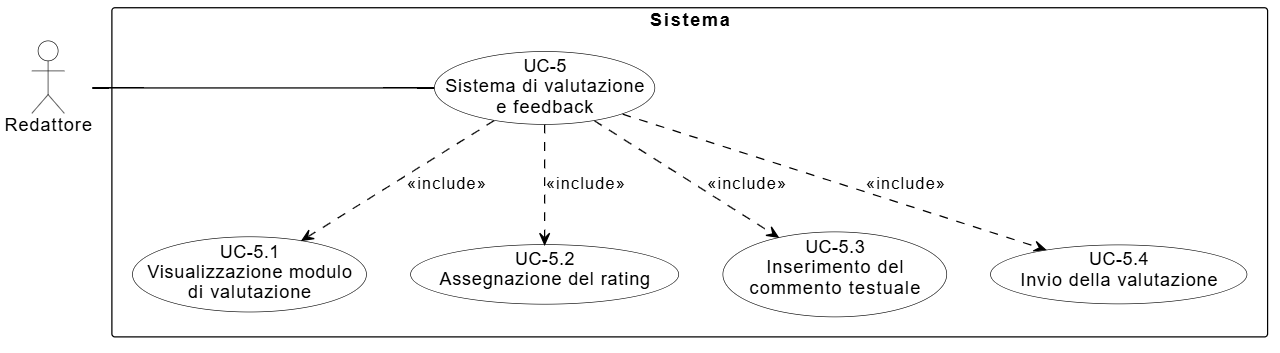
\includegraphics[width=1.15\textwidth]{diagrammi_use_case/UC-5.png}
    \caption{Diagramma del caso d'uso UC-5: Sistema di valutazione e feedback}
    \label{fig:uc-5}
\end{figure}
\begin{description}[style=multiline, leftmargin=4.5cm, font=\bfseries]
    
    \item[\glslink{attore}{Attore} Principale] \glslink{redattore}{Redattore}
    
    \item[\glslink{trigger}{Trigger}] Il \glslink{redattore}{Redattore} intende fornire un riscontro qualitativo sulla \glslink{bozza-draft}{bozza} generata.

    \item[Pre-condizioni] Il sistema ha completato la generazione dell'output (UC-1) e abilita le funzionalità di raccolta feedback. La fornitura del feedback è un'azione completamente opzionale (UC-3).
    
    \item[Post-condizioni] Il feedback (punteggio ed eventuale commento) è archiviato nel sistema in associazione alla \glslink{bozza-draft}{bozza} valutata.
    
    \item[\glslink{scenario-principale}{Scenario Principale}] 
    \begin{enumerate}[leftmargin=*, nosep]
        \item Il \glslink{redattore}{Redattore} visualizza il modulo di valutazione a schermo (\textbf{UC-5.1}).
        \item Il \glslink{redattore}{Redattore} assegna un punteggio di gradimento tramite il selettore grafico (\textbf{UC-5.2}).
        \item Il \glslink{redattore}{Redattore} inserisce una nota testuale per dettagliare il feedback (\textbf{UC-5.3}).
        \item Il \glslink{redattore}{Redattore} conferma l'invio della valutazione (\textbf{UC-5.4}).
    \end{enumerate}

    \item[Relazioni] 
    \begin{itemize}[leftmargin=*, nosep]
        \item \textbf{Inclusioni}: UC-5.1, UC-5.2, UC-5.3, UC-5.4.
    \end{itemize}
\end{description}

\paragraph{UC-5.1: Visualizzazione del modulo di valutazione}
\mbox{} \\

\begin{figure}[H]
    \centering
    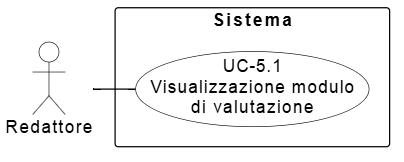
\includegraphics[width=0.5\textwidth]{diagrammi_use_case/UC-5.1.png}
    \caption{Diagramma del caso d'uso UC-5.1: Visualizzazione del modulo di valutazione}
    \label{fig:uc-5.1}
\end{figure}
\begin{description}[style=multiline, leftmargin=4cm, font=\bfseries]
    \item[\glslink{attore}{Attore} Principale] \glslink{redattore}{Redattore}
    \item[Pre-condizioni] Il sistema ha esposto a schermo il contenuto generato o in fase di revisione.
    \item[Post-condizioni] Il \glslink{redattore}{Redattore} visualizza l'interfaccia dedicata alla raccolta del feedback.
    \item[\glslink{scenario-principale}{Scenario Principale}] 
    \begin{enumerate}[leftmargin=*, nosep]
        \item Il sistema rende visibile il modulo comprendente il selettore di \glslink{rating}{rating} e il campo testuale opzionale.
    \end{enumerate}
\end{description}

\paragraph{UC-5.2: Assegnazione del rating}
\mbox{} \\

\begin{figure}[H]
    \centering
    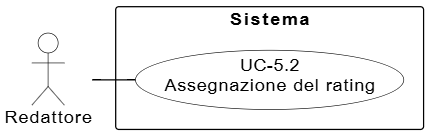
\includegraphics[width=0.5\textwidth]{diagrammi_use_case/UC-5.2.png}
    \caption{Diagramma del caso d'uso UC-5.2: Assegnazione del rating}
    \label{fig:uc-5.2}
\end{figure}
\begin{description}[style=multiline, leftmargin=4cm, font=\bfseries]
    \item[\glslink{attore}{Attore} Principale] \glslink{redattore}{Redattore}
    \item[Pre-condizioni] Il sistema espone il selettore grafico di valutazione.
    \item[Post-condizioni] Il sistema ha registrato temporaneamente il punteggio selezionato.
    \item[\glslink{scenario-principale}{Scenario Principale}] 
    \begin{enumerate}[leftmargin=*, nosep]
        \item Il \glslink{redattore}{Redattore} seleziona il punteggio desiderato interagendo con il selettore.
        \item Il sistema evidenzia graficamente la selezione effettuata per fornire un feedback visivo.
    \end{enumerate}
\end{description}

\paragraph{UC-5.3: Inserimento del commento testuale}
\mbox{} \\

\begin{figure}[H]
    \centering
    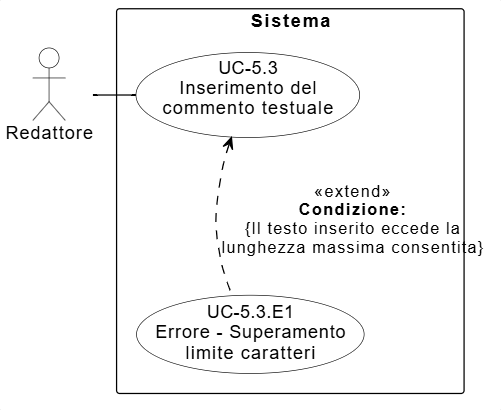
\includegraphics[width=0.9\textwidth]{diagrammi_use_case/UC-5.3.png}
    \caption{Diagramma del caso d'uso UC-5.3: Inserimento del commento testuale}
    \label{fig:uc-5.3}
\end{figure}
\begin{description}[style=multiline, leftmargin=4cm, font=\bfseries]
    \item[\glslink{attore}{Attore} Principale] \glslink{redattore}{Redattore}
    \item[Pre-condizioni] Il sistema espone il campo di testo opzionale per la motivazione del voto.
    \item[Post-condizioni] Il sistema ha registrato temporaneamente il testo inserito.
    \item[\glslink{scenario-principale}{Scenario Principale}] 
    \begin{enumerate}[leftmargin=*, nosep]
        \item Il \glslink{redattore}{Redattore} seleziona l'area di input testuale.
        \item Il \glslink{redattore}{Redattore} inserisce il proprio commento o suggerimento qualitativo.
    \end{enumerate}
    \item[Scenari Alternativi] 
    \begin{itemize}[leftmargin=*, nosep]
        \item \textbf{2a. Superamento limite caratteri}: Il sistema rileva che il testo inserito eccede la lunghezza massima consentita; viene eseguito \textbf{UC-5.3.E1}.
    \end{itemize}

    \item[Relazioni] 
    \begin{itemize}[leftmargin=*, nosep]
        \item \textbf{Estensioni}: UC-5.3.E1.
    \end{itemize}
\end{description}

\paragraph{UC-5.4: Invio della valutazione}
\mbox{} \\
\begin{figure}[H]
    \centering
    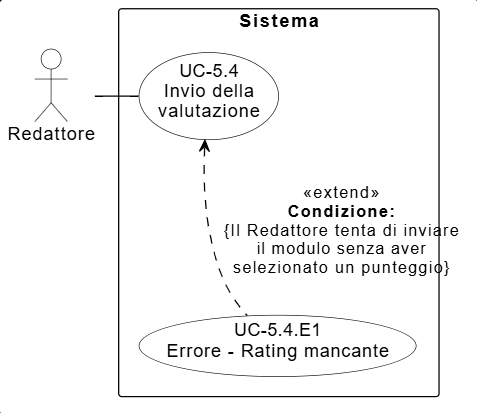
\includegraphics[width=0.9\textwidth]{diagrammi_use_case/UC-5.4.png}
    \caption{Diagramma del caso d'uso UC-5.4: Invio della valutazione}
    \label{fig:uc-5.4}
\end{figure}
\begin{description}[style=multiline, leftmargin=4.5cm, font=\bfseries]
    \item[\glslink{attore}{Attore} Principale] \glslink{redattore}{Redattore}
    \item[Pre-condizioni] Il \glslink{redattore}{Redattore} ha compilato il dato obbligatorio del modulo (\glslink{rating}{rating}).
    \item[Post-condizioni] La valutazione è stata acquisita dal sistema e il modulo è disabilitato per la \glslink{bozza-draft}{bozza} corrente.
    \item[\glslink{scenario-principale}{Scenario Principale}] 
    \begin{enumerate}[leftmargin=*, nosep]
        \item Il \glslink{redattore}{Redattore} seleziona il comando di invio del feedback.
        \item Il sistema conferma l'acquisizione dei dati visualizzando un messaggio di ringraziamento.
        \item Il sistema disabilita permanentemente il modulo di feedback per la generazione corrente, al fine di prevenire votazioni multiple.
    \end{enumerate}
    \item[Scenari Alternativi] 
    \begin{itemize}[leftmargin=*, nosep]
        \item \textbf{1a. \glslink{rating}{Rating} mancante}: Il sistema rileva che il \glslink{redattore}{Redattore} tenta di inviare il modulo senza aver selezionato un punteggio; viene eseguito \textbf{UC-5.4.E1}.
    \end{itemize}

    \item[Relazioni] 
    \begin{itemize}[leftmargin=*, nosep]
        \item \textbf{Estensioni}: UC-5.4.E1.
    \end{itemize}
\end{description}

\paragraph{UC-5.4.E1: Errore - Rating mancante}
\mbox{} \\

\begin{figure}[H]
    \centering
    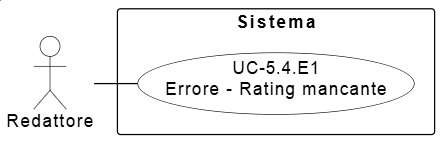
\includegraphics[width=0.6\textwidth]{diagrammi_use_case/UC-5.E1.png}
    \caption{Diagramma del caso d'uso UC-5.4.E1: Errore per rating mancante}
    \label{fig:uc-5.4.e1}
\end{figure}
\begin{description}[style=multiline, leftmargin=4cm, font=\bfseries]
    \item[\glslink{attore}{Attore} Principale] \glslink{redattore}{Redattore}
    \item[Pre-condizioni] Il \glslink{redattore}{Redattore} seleziona il comando di invio mantenendo lo stato del \glslink{rating}{rating} vuoto (0 su 5).
    \item[Post-condizioni] Il sistema blocca la procedura di invio e mantiene il modulo attivo.
    \item[\glslink{scenario-principale}{Scenario Principale}] 
    \begin{enumerate}[leftmargin=*, nosep]
        \item Il sistema interrompe l'operazione di salvataggio.
        \item Il sistema evidenzia visivamente il selettore del punteggio, segnalandone l'obbligatorietà.
        \item Il sistema invita il \glslink{redattore}{Redattore} a selezionare un valore prima di procedere.
    \end{enumerate}
\end{description}

\paragraph{UC-5.3.E1: Errore - Superamento limite caratteri}
\mbox{} \\

\begin{figure}[H]
    \centering
    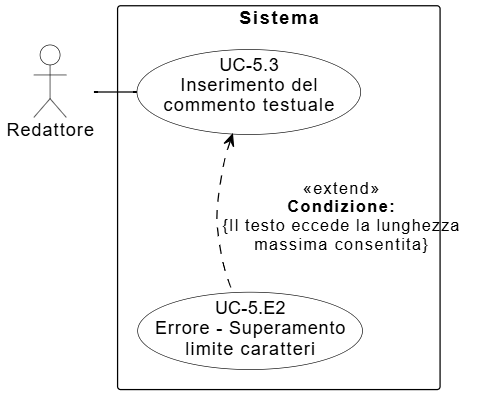
\includegraphics[width=0.5\textwidth]{diagrammi_use_case/UC-5.E2.png}
    \caption{Diagramma del caso d'uso UC-5.3.E1: Errore per superamento limite caratteri}
    \label{fig:uc-5.3.e1}
\end{figure}
\begin{description}[style=multiline, leftmargin=4cm, font=\bfseries]
    \item[\glslink{attore}{Attore} Principale] \glslink{redattore}{Redattore}
    \item[Pre-condizioni] Il \glslink{redattore}{Redattore} sta digitando il commento e raggiunge il limite massimo di caratteri consentito dal sistema.
    \item[Post-condizioni] Il sistema preserva il testo fino al limite e non accetta ulteriori input.
    \item[\glslink{scenario-principale}{Scenario Principale}] 
    \begin{enumerate}[leftmargin=*, nosep]
        \item Il sistema inibisce la digitazione di nuovi caratteri all'interno del campo.
        \item Il sistema mostra un avviso visivo relativo al raggiungimento della lunghezza massima.
    \end{enumerate}
\end{description} 
\newpage
\subsubsection{UC-6: Dashboard metriche e monitoraggio}
\mbox{} \\

\begin{figure}[H]
    \centering
    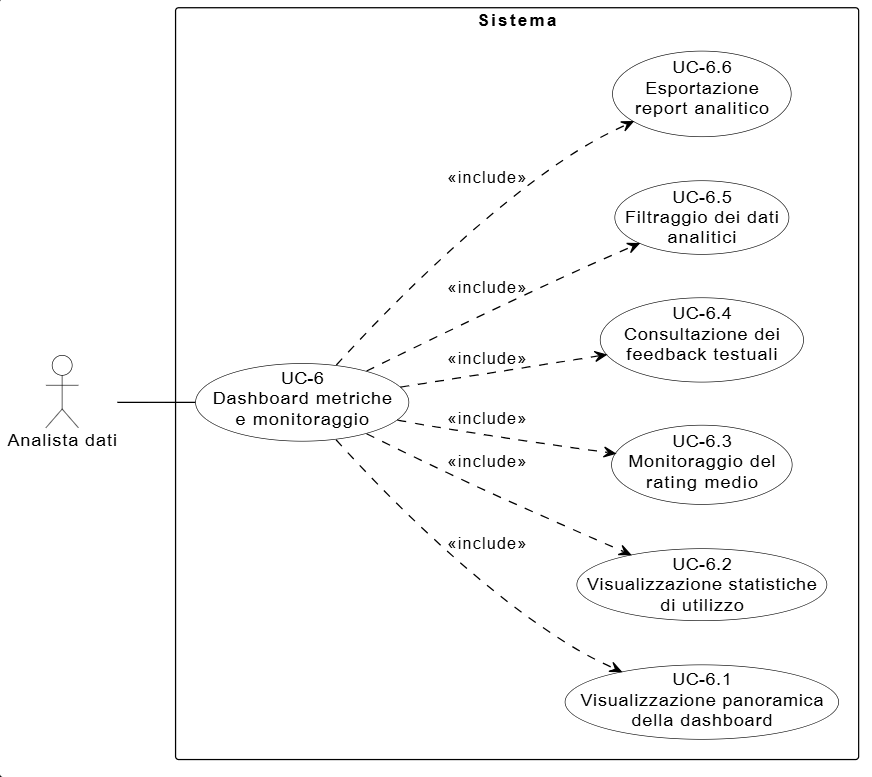
\includegraphics[width=0.9\textwidth]{diagrammi_use_case/UC-6.png}
    \caption{Diagramma del caso d'uso UC-6: Dashboard metriche e monitoraggio}
    \label{fig:uc-6}
\end{figure}
\begin{description}[style=multiline, leftmargin=4cm, font=\bfseries]
    \item[\glslink{attore}{Attore} Principale] \glslink{analista-dati}{Analista dati}
    
    \item[\glslink{trigger}{Trigger}] L'\glslink{analista-dati}{Analista dati} accede all'area analitica per monitorare le performance e l'utilizzo dell'\glslink{intelligenza-artificiale-ai}{AI} Assistant.

    \item[Pre-condizioni] Il sistema ha archiviato i dati di utilizzo dell'Assistente \glslink{intelligenza-artificiale-ai}{AI} e le valutazioni qualitative degli utenti.
    
    \item[Post-condizioni] L'\glslink{analista-dati}{Analista dati} ha consultato le metriche e ha avuto la possibilità di filtrare o esportare i dati analitici.
    
    \item[\glslink{scenario-principale}{Scenario Principale}] 
    \begin{enumerate}[leftmargin=*, nosep]
        \item L'\glslink{analista-dati}{Analista dati} accede alla \glslink{dashboard}{dashboard} e visualizza la panoramica delle metriche (\textbf{UC-6.1}).
        \item L'\glslink{analista-dati}{Analista dati} consulta le statistiche operative di utilizzo (\textbf{UC-6.2}).
        \item L'\glslink{analista-dati}{Analista dati} monitora il livello di \glslink{rating}{rating} medio (\textbf{UC-6.3}).
        \item L'\glslink{analista-dati}{Analista dati} consulta la lista dei feedback testuali (\textbf{UC-6.4}).
        \item L'\glslink{analista-dati}{Analista dati} applica filtri dinamici \glslink{intelligenza-artificiale-ai}{ai} dati visualizzati (\textbf{UC-6.5}).
        \item L'\glslink{analista-dati}{Analista dati} richiede l'esportazione del report analitico (\textbf{UC-6.6}).
    \end{enumerate}

    \item[Relazioni] 
    \begin{itemize}[leftmargin=*, nosep]
        \item \textbf{Inclusioni}: UC-6.1, UC-6.2, UC-6.3, UC-6.4, UC-6.5, UC-6.6.
    \end{itemize}

\end{description}

\paragraph{UC-6.1: Visualizzazione panoramica della dashboard}
\mbox{} \\

\begin{figure}[H]
    \centering
    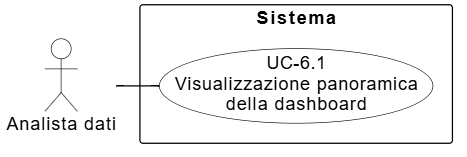
\includegraphics[width=0.6\textwidth]{diagrammi_use_case/UC-6.1.png}
    \caption{Diagramma del caso d'uso UC-6.1: Visualizzazione panoramica della dashboard}
    \label{fig:uc-6.1}
\end{figure}
\begin{description}[style=multiline, leftmargin=4cm, font=\bfseries]
    \item[\glslink{attore}{Attore} Principale] \glslink{analista-dati}{Analista dati}
    \item[Pre-condizioni] L'\glslink{analista-dati}{Analista dati} accede all'area analitica del sistema.
    \item[Post-condizioni] Il sistema espone l'interfaccia riepilogativa delle metriche.
    \item[\glslink{scenario-principale}{Scenario Principale}] 
    \begin{enumerate}[leftmargin=*, nosep]
        \item Il sistema presenta a schermo l'interfaccia di monitoraggio con i principali indicatori di performance dell'\glslink{intelligenza-artificiale-ai}{AI} Assistant.
    \end{enumerate}
\end{description}

\paragraph{UC-6.2: Visualizzazione statistiche di utilizzo}
\mbox{} \\

\begin{figure}[H]
    \centering
    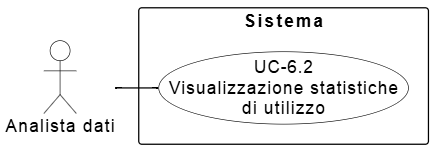
\includegraphics[width=0.6\textwidth]{diagrammi_use_case/UC-6.2.png}
    \caption{Diagramma del caso d'uso UC-6.2: Visualizzazione statistiche di utilizzo}
    \label{fig:uc-6.2}
\end{figure}
\begin{description}[style=multiline, leftmargin=4cm, font=\bfseries]
    \item[\glslink{attore}{Attore} Principale] \glslink{analista-dati}{Analista dati}
    \item[Pre-condizioni] L'\glslink{analista-dati}{Analista dati} si trova all'interno della \glslink{dashboard}{dashboard}.
    \item[Post-condizioni] Il sistema mostra i contatori operativi aggiornati.
    \item[\glslink{scenario-principale}{Scenario Principale}] 
    \begin{enumerate}[leftmargin=*, nosep]
        \item Il sistema visualizza i dati quantitativi relativi all'utilizzo (numero di contenuti generati e \glslink{prompt}{prompt} salvati).
    \end{enumerate}
\end{description}

\paragraph{UC-6.3: Monitoraggio del rating medio}
\mbox{} \\

\begin{figure}[H]
    \centering
    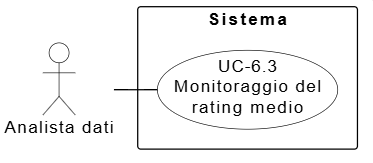
\includegraphics[width=0.5\textwidth]{diagrammi_use_case/UC-6.3.png}
    \caption{Diagramma del caso d'uso UC-6.3: Monitoraggio del rating medio}
    \label{fig:uc-6.3}
\end{figure}
\begin{description}[style=multiline, leftmargin=4cm, font=\bfseries]
    \item[\glslink{attore}{Attore} Principale] \glslink{analista-dati}{Analista dati}
    \item[Pre-condizioni] Sono presenti nel sistema feedback numerici espressi dai Redattori (UC-5).
    \item[Post-condizioni] Il sistema mostra l'indicatore della qualità percepita.
    \item[\glslink{scenario-principale}{Scenario Principale}] 
    \begin{enumerate}[leftmargin=*, nosep]
        \item Il sistema visualizza il valore medio delle valutazioni a stelle ricevute per misurare l'efficacia dell'\glslink{intelligenza-artificiale-ai}{AI}.
    \end{enumerate}
\end{description}

\paragraph{UC-6.4: Consultazione dei feedback testuali}
\mbox{} \\

\begin{figure}[H]
    \centering
    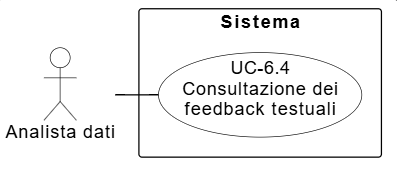
\includegraphics[width=0.5\textwidth]{diagrammi_use_case/UC-6.4.png}
    \caption{Diagramma del caso d'uso UC-6.4: Consultazione dei feedback testuali}
    \label{fig:uc-6.4}
\end{figure}
\begin{description}[style=multiline, leftmargin=4cm, font=\bfseries]
    \item[\glslink{attore}{Attore} Principale] \glslink{analista-dati}{Analista dati}
    \item[Pre-condizioni] Sono presenti nel sistema commenti testuali associati alle valutazioni.
    \item[Post-condizioni] L'\glslink{analista-dati}{Analista dati} ha consultato le note qualitative dei Redattori.
    \item[\glslink{scenario-principale}{Scenario Principale}] 
    \begin{enumerate}[leftmargin=*, nosep]
        \item Il sistema visualizza direttamente nella \glslink{dashboard}{dashboard} la lista dei feedback più recenti, comprensivi di punteggio a stelle e commento testuale.
    \end{enumerate}
\end{description}

\paragraph{UC-6.5: Filtraggio dei dati analitici}
\mbox{} \\
\begin{figure}[H]
    \centering
    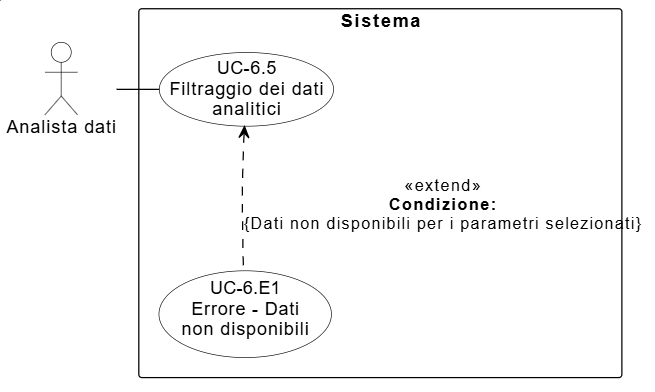
\includegraphics[width=1\textwidth]{diagrammi_use_case/UC-6.5.png}
    \caption{Diagramma del caso d'uso UC-6.5: Filtraggio dei dati analitici}
    \label{fig:uc-6.5}
\end{figure}
\begin{description}[style=multiline, leftmargin=4.5cm, font=\bfseries]
    \item[\glslink{attore}{Attore} Principale] \glslink{analista-dati}{Analista dati}
    \item[Pre-condizioni] L'\glslink{analista-dati}{Analista dati} visualizza i dati all'interno della \glslink{dashboard}{dashboard}.
    \item[Post-condizioni] Il sistema aggiorna la visualizzazione in base \glslink{intelligenza-artificiale-ai}{ai} parametri selezionati.
    \item[\glslink{scenario-principale}{Scenario Principale}] 
    \begin{enumerate}[leftmargin=*, nosep]
        \item L'\glslink{analista-dati}{Analista dati} imposta parametri specifici di filtro (es. intervallo di date, tono, stile).
        \item Il sistema aggiorna istantaneamente la visualizzazione in base \glslink{intelligenza-artificiale-ai}{ai} criteri scelti.
    \end{enumerate}
    \item[Scenari Alternativi] 
    \begin{itemize}[leftmargin=*, nosep]
        \item \textbf{2a. Dati non disponibili}: Il sistema rileva l'assenza di record corrispondenti \glslink{intelligenza-artificiale-ai}{ai} filtri applicati; viene eseguito \textbf{UC-6.E1}.
    \end{itemize}
    \item[Relazioni] 
    \begin{itemize}[leftmargin=*, nosep]
        \item \textbf{Estensioni}: UC-6.E1.
    \end{itemize}
\end{description}

\paragraph{UC-6.6: Esportazione report analitico}
\mbox{} \\

\begin{figure}[H]
    \centering
    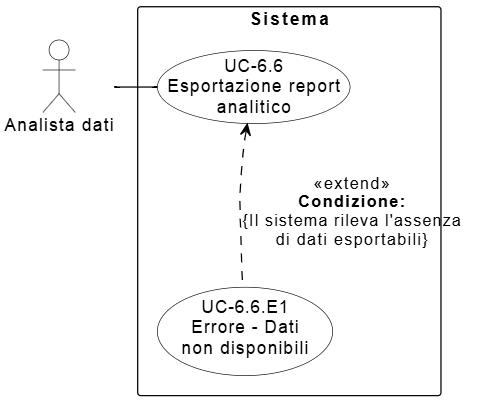
\includegraphics[width=1\textwidth]{diagrammi_use_case/UC-6.6.png}
    \caption{Diagramma del caso d'uso UC-6.6: Esportazione report analitico}
    \label{fig:uc-6.6}
\end{figure}
\begin{description}[style=multiline, leftmargin=4cm, font=\bfseries]
    \item[\glslink{attore}{Attore} Principale] \glslink{analista-dati}{Analista dati}
    \item[Pre-condizioni] Il sistema espone i comandi di esportazione dati.
    \item[Post-condizioni] Il sistema ha fornito un file scaricabile localmente.
    \item[\glslink{scenario-principale}{Scenario Principale}] 
    \begin{enumerate}[leftmargin=*, nosep]
        \item L'\glslink{analista-dati}{Analista dati} seleziona il comando di esportazione.
        \item Il sistema avvia il download del documento riepilogativo sul dispositivo dell'utente.
    \end{enumerate}
    \item[Scenari Alternativi] 
    \begin{itemize}[leftmargin=*, nosep]
        \item \textbf{2a. Dati non disponibili}: Il sistema rileva l'assenza di dati esportabili; viene eseguito \textbf{UC-6.6.E1}.
    \end{itemize}
    \item[Relazioni] 
    \begin{itemize}[leftmargin=*, nosep]
        \item \textbf{Estensioni}: UC-6.6.E1.
    \end{itemize}
\end{description}

\paragraph{UC-6.6.E1: Errore - Dati non disponibili}
\mbox{} \\

\begin{figure}[H]
    \centering
    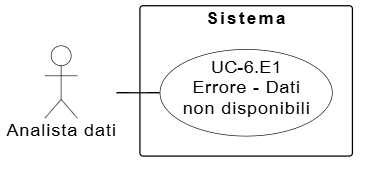
\includegraphics[width=0.45\textwidth]{diagrammi_use_case/UC-6.E1.png}
    \caption{Diagramma del caso d'uso UC-6.6.E1: Errore per dati non disponibili}
    \label{fig:uc-6.6.e1}
\end{figure}
\begin{description}[style=multiline, leftmargin=4cm, font=\bfseries]
    \item[\glslink{attore}{Attore} Principale] \glslink{analista-dati}{Analista dati}
    \item[Pre-condizioni] L'\glslink{analista}{Analista} applica filtri o richiede esportazioni per parametri privi di interazioni registrate.
    \item[Post-condizioni] Il sistema segnala l'assenza di dati e permette di modificare i criteri.
    \item[\glslink{scenario-principale}{Scenario Principale}] 
    \begin{enumerate}[leftmargin=*, nosep]
        \item Il sistema segnala l'impossibilità di procedere a causa della mancanza di dati per il periodo o i filtri selezionati.
        \item Il sistema visualizza un messaggio di avviso e invita l'\glslink{analista}{Analista} a modificare i parametri di ricerca.
    \end{enumerate}
\end{description}
\newpage
\subsection{AI Co-Pilot per Consulenti del Lavoro}

\subsubsection{UC-7: Upload del documento}
\mbox{} \\

\begin{figure}[H]
    \centering
    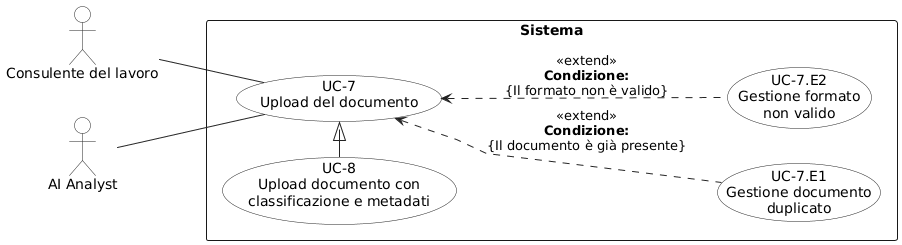
\includegraphics[width=1.1\textwidth]{diagrammi_use_case/uc_7.png}
    \caption{Diagramma del caso d'uso UC-7: Upload del documento}
    \label{fig:uc-7}
\end{figure}
\begin{description}[style=multiline, leftmargin=4cm, font=\bfseries]
    
    \item[\glslink{attore}{Attore} Principale] \glslink{consulente-del-lavoro-cdl}{Consulente del lavoro}
    \item[\glslink{attore-secondario}{Attore Secondario}] \glslink{ai-analyst}{AI Analyst}
    
    \item[\glslink{trigger}{Trigger}] Il \glslink{consulente-del-lavoro-cdl}{Consulente del lavoro} intende caricare uno o più documenti nel sistema.
    
    \item[Pre-condizioni] Il \glslink{consulente-del-lavoro-cdl}{Consulente del lavoro} si trova nella sezione di upload del modulo \glslink{intelligenza-artificiale-ai}{AI} Co-Pilot.
    
    \item[Post-condizioni]Il documento è caricato e analizzato dall'\glslink{intelligenza-artificiale-ai}{AI} (estrazione \glslink{metadati}{metadati}, classificazione e split in sotto-documenti per destinatario).
   
    \item[\glslink{scenario-principale}{Scenario Principale}] 
    \begin{enumerate}[leftmargin=*, nosep]
        \item Il \glslink{consulente-del-lavoro-cdl}{Consulente del lavoro} seleziona il file dal proprio dispositivo.
        \item Il \glslink{consulente-del-lavoro-cdl}{Consulente del lavoro} conferma il caricamento.
        \item Il sistema verifica formato e duplicati.
        \item Il sistema completa il caricamento, notifica l'esito positivo e avvia l'analisi \glslink{intelligenza-artificiale-ai}{AI} del documento.
    \end{enumerate}

    \item[Scenari Alternativi]
    \begin{itemize}[leftmargin=*, nosep]
        \item 3a. Documento duplicato: Il sistema rileva che il file è già presente; viene eseguito UC-7.E1.
        \item 3b. Formato non valido: Il sistema rileva un formato non supportato; viene eseguito UC-7.E2.
    \end{itemize}

    \item[Relazioni]
    \begin{itemize}[leftmargin=*, nosep]
        \item \textbf{Generalizzazioni}: UC-8.
        \item \textbf{Estensioni}: UC-7.E1, UC-7.E2.
    \end{itemize}

\end{description}

\paragraph{UC-7.E1: Gestione documento duplicato}
\mbox{} \\

\begin{figure}[H]
    \centering
    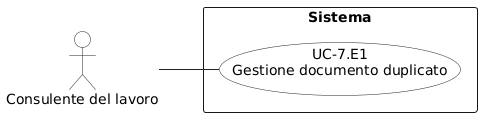
\includegraphics[width=0.7\textwidth]{diagrammi_use_case/uc_7.E1.png}
    \caption{Diagramma del caso d'uso UC-7.E1: Gestione documento duplicato}
    \label{fig:uc-7.e1}
\end{figure}
\begin{description}[style=multiline, leftmargin=4cm, font=\bfseries]
    \item[\glslink{attore}{Attore} Principale] \glslink{consulente-del-lavoro-cdl}{Consulente del lavoro}
    \item[Pre-condizioni] Durante la verifica di caricamento, il sistema rileva che il documento è già presente in archivio.
    \item[Post-condizioni] Il sistema gestisce la scelta dell'utente: in caso di conferma il documento viene caricato, altrimenti l'archivio resta invariato.
    \item[\glslink{scenario-principale}{Scenario Principale}]
    \begin{enumerate}[leftmargin=*, nosep]
        \item Il sistema segnala che il documento risulta gia' presente in archivio.
        \item Il sistema richiede conferma per procedere con il caricamento del duplicato.
        \item Il \glslink{consulente-del-lavoro-cdl}{Consulente del lavoro} conferma o annulla il caricamento.
    \end{enumerate}
\end{description}

\paragraph{UC-7.E2: Gestione formato non valido}
\mbox{} \\

\begin{figure}[H]
    \centering
    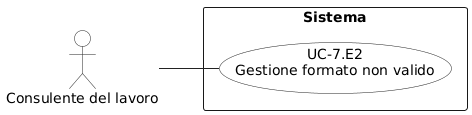
\includegraphics[width=0.7\textwidth]{diagrammi_use_case/uc_7.E2.png}
    \caption{Diagramma del caso d'uso UC-7.E2: Gestione formato non valido}
    \label{fig:uc-7.e2}
\end{figure}
\begin{description}[style=multiline, leftmargin=4cm, font=\bfseries]
    \item[\glslink{attore}{Attore} Principale] \glslink{consulente-del-lavoro-cdl}{Consulente del lavoro}
    \item[Pre-condizioni] Durante la verifica di caricamento, il sistema rileva che il formato del file non è supportato.
    \item[Post-condizioni] Il documento non viene caricato e il sistema richiede un nuovo file in formato valido.
    \item[\glslink{scenario-principale}{Scenario Principale}]
    \begin{enumerate}[leftmargin=*, nosep]
        \item Il sistema interrompe la procedura di caricamento del documento.
        \item Il sistema mostra un messaggio di errore indicando i formati supportati.
    \end{enumerate}
\end{description}

\subsubsection{UC-8: Upload documento con classificazione e metadati}
\mbox{} \\

\begin{figure}[H]
    \centering
    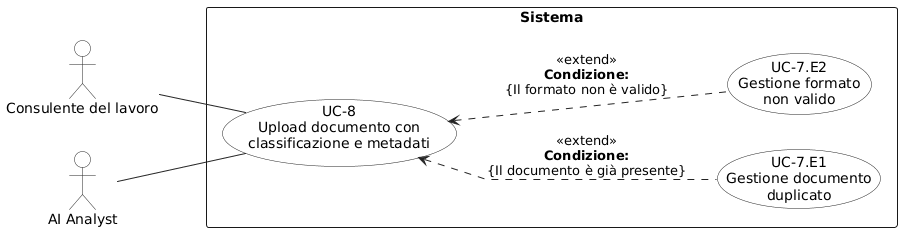
\includegraphics[width=1.1\textwidth]{diagrammi_use_case/uc_8.png}
    \caption{Diagramma del caso d'uso UC-8: Upload documento con classificazione e metadati}
    \label{fig:uc-8}
\end{figure}
\begin{description}[style=multiline, leftmargin=4cm, font=\bfseries]
    \item[\glslink{attore}{Attore} Principale] \glslink{consulente-del-lavoro-cdl}{Consulente del lavoro}
    \item[\glslink{attore-secondario}{Attore Secondario}] \glslink{ai-analyst}{AI Analyst}
    \item[\glslink{trigger}{Trigger}] Il \glslink{consulente-del-lavoro-cdl}{Consulente del lavoro} intende caricare uno o più documenti nel sistema impostando manualmente classificazione e \glslink{metadati}{metadati}.
    \item[Pre-condizioni] Il \glslink{consulente-del-lavoro-cdl}{Consulente del lavoro} si trova nella sezione di upload del modulo \glslink{intelligenza-artificiale-ai}{AI} Co-Pilot.   
    \item[Post-condizioni] Il documento è caricato e analizzato dall'\glslink{intelligenza-artificiale-ai}{AI}; classificazione e \glslink{metadati}{metadati} inseriti manualmente non vengono ricalcolati mentre viene già eseguito lo split (del documento in sotto-documenti per destinatario).

    \item[\glslink{scenario-principale}{Scenario Principale}]
    \begin{enumerate}[leftmargin=*, nosep]
        \item Il \glslink{consulente-del-lavoro-cdl}{Consulente del lavoro} seleziona il file dal proprio dispositivo.
        \item Il \glslink{consulente-del-lavoro-cdl}{Consulente del lavoro} seleziona la tipologia del documento tra le opzioni disponibili: cedolino, CU, comunicazione, documento da firmare, lettera, altro.
        \item Il \glslink{consulente-del-lavoro-cdl}{Consulente del lavoro} seleziona il formato file tra le opzioni disponibili: PDF, PNG, JPG e TIFF.
        \item Il \glslink{consulente-del-lavoro-cdl}{Consulente del lavoro} inserisce i \glslink{metadati}{metadati} richiesti (mese, anno, azienda).
        \item Il \glslink{consulente-del-lavoro-cdl}{Consulente del lavoro} conferma il caricamento dopodiché il sistema verifica formato e duplicati.
        \item Il sistema completa il caricamento, avvia l'analisi \glslink{intelligenza-artificiale-ai}{AI} del documento e mantiene i campi inseriti dall'utente.
    \end{enumerate}
    \item[Scenari Alternativi]
    \begin{itemize}[leftmargin=*, nosep]
        \item 4a. Documento duplicato: il sistema rileva che il file è già presente; viene eseguito UC-7.E1.
        \item 4b. Formato non valido: il sistema rileva un formato non supportato; viene eseguito UC-7.E2.
    \end{itemize}
    \item[Relazioni]
    \begin{itemize}[leftmargin=*, nosep]
        \item \textbf{Estensioni}: UC-7.E1, UC-7.E2.
    \end{itemize}
\end{description}


\subsubsection{UC-9: Visualizzazione storico documenti analizzati}
\mbox{} \\

\begin{figure}[H]
    \centering
    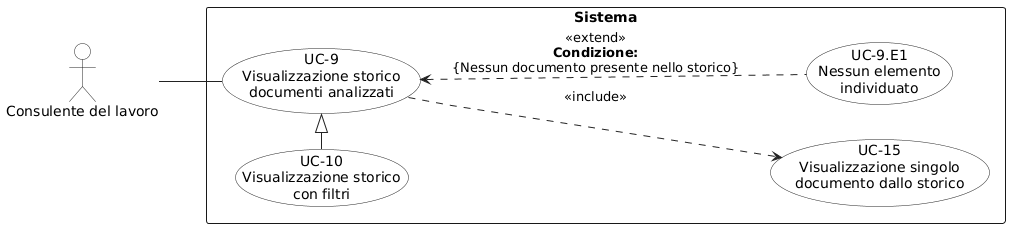
\includegraphics[width=1.1\textwidth]{diagrammi_use_case/uc_9.png}
    \caption{Diagramma del caso d'uso UC-9: Visualizzazione storico documenti analizzati}
    \label{fig:uc-9}
\end{figure}
\begin{description}[style=multiline, leftmargin=4cm, font=\bfseries]
    \item[\glslink{attore}{Attore} Principale] \glslink{consulente-del-lavoro-cdl}{Consulente del lavoro}
    \item[\glslink{trigger}{Trigger}] Il \glslink{consulente-del-lavoro-cdl}{Consulente del lavoro} intende consultare lo storico dei documenti analizzati nel modulo \glslink{intelligenza-artificiale-ai}{AI} Co-Pilot.
    \item[Pre-condizioni] Il \glslink{consulente-del-lavoro-cdl}{Consulente del lavoro} si trova nel modulo \glslink{intelligenza-artificiale-ai}{AI} Co-Pilot e apre la sezione "Storico documenti".
    \item[Post-condizioni] Il sistema mostra l'elenco dei documenti analizzati e permette la consultazione del dettaglio del singolo elemento selezionato.
    \item[\glslink{scenario-principale}{Scenario Principale}]
    \begin{enumerate}[leftmargin=*, nosep]
        \item Il \glslink{consulente-del-lavoro-cdl}{Consulente del lavoro} accede alla sezione "Storico documenti analizzati".
        \item Il sistema recupera e visualizza di default i documenti più recentemente analizzati, ordinati secondo l'ordine di richiesta di analisi (dal più recente al meno recente).
        \item Il \glslink{consulente-del-lavoro-cdl}{Consulente del lavoro} seleziona un elemento della lista per consultarne i dettagli (\textbf{UC-15}).
    \end{enumerate}
    \item[Scenari Alternativi]
    \begin{itemize}[leftmargin=*, nosep]
        \item 2a. Nessun elemento individuato: il sistema non trova documenti corrispondenti nello storico; viene eseguito UC-9.E1.
    \end{itemize}
    \item[Relazioni]
    \begin{itemize}[leftmargin=*, nosep]
        \item \textbf{Inclusioni}: UC-15.
        \item \textbf{Generalizzazioni}: UC-10.
        \item \textbf{Estensioni}: UC-9.E1.
    \end{itemize}
\end{description}
\newpage
\paragraph{UC-9.E1: Nessun elemento individuato}
\mbox{} \\

\begin{figure}[H]
    \centering
    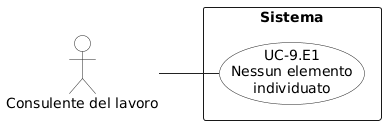
\includegraphics[width=0.6\textwidth]{diagrammi_use_case/uc_9.E1.png}
    \caption{Diagramma del caso d'uso UC-9.E1: Nessun elemento individuato}
    \label{fig:uc-9.e1}
\end{figure}
\begin{description}[style=multiline, leftmargin=4cm, font=\bfseries]
    \item[\glslink{attore}{Attore} Principale] \glslink{consulente-del-lavoro-cdl}{Consulente del lavoro}
    \item[Pre-condizioni] Il \glslink{consulente-del-lavoro-cdl}{Consulente del lavoro} accede allo storico o applica filtri e non è presente alcun documento corrispondente.
    \item[Post-condizioni] Il sistema mantiene attiva la schermata dello storico e informa l'utente dell'assenza di elementi.
    \item[\glslink{scenario-principale}{Scenario Principale}]
    \begin{enumerate}[leftmargin=*, nosep]
        \item Il sistema rileva che non c'è alcun elemento individuato.
        \item Il sistema visualizza un avviso di storico vuoto e propone di caricare nuovi documenti o di azzerare eventuali filtri.
    \end{enumerate}
\end{description}
\newpage
\subsubsection{UC-10: Visualizzazione storico con filtri}
\mbox{} \\

\begin{figure}[H]
    \centering
    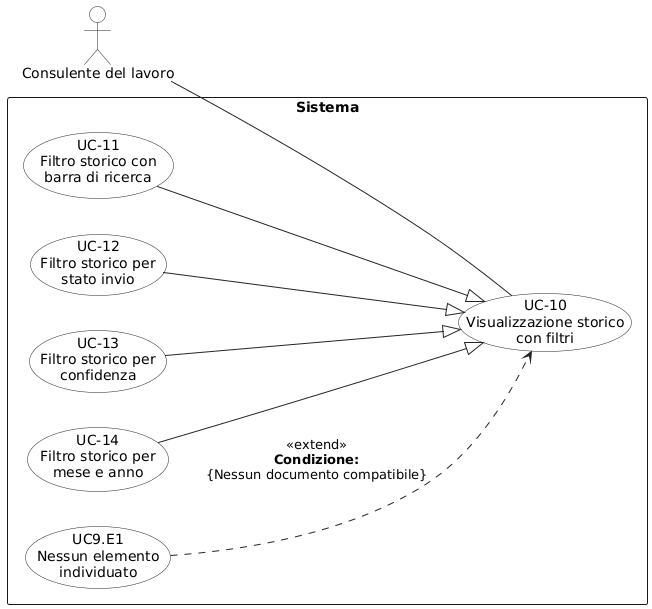
\includegraphics[width=0.9\textwidth]{diagrammi_use_case/uc_10.png}
    \caption{Diagramma del caso d'uso UC-10: Visualizzazione storico con filtri}
    \label{fig:uc-10}
\end{figure}
\begin{description}[style=multiline, leftmargin=4cm, font=\bfseries]
    \item[\glslink{attore}{Attore} Principale] \glslink{consulente-del-lavoro-cdl}{Consulente del lavoro}
    \item[\glslink{trigger}{Trigger}] Il \glslink{consulente-del-lavoro-cdl}{Consulente del lavoro} intende restringere lo storico dei documenti analizzati applicando uno o più filtri.
    \item[Pre-condizioni] Il \glslink{consulente-del-lavoro-cdl}{Consulente del lavoro} si trova nella sezione "Storico documenti analizzati".
    \item[Post-condizioni] Il sistema mostra un sottoinsieme dello storico coerente con i filtri applicati.
    \item[\glslink{scenario-principale}{Scenario Principale}]
    \begin{enumerate}[leftmargin=*, nosep]
        \item Il \glslink{consulente-del-lavoro-cdl}{Consulente del lavoro} imposta uno o più filtri tra i proposti: barra di ricerca (\textbf{UC-11}), stato invio (\textbf{UC-12}), \glslink{confidenza-confidence-score}{confidenza} rispetto a soglia (\textbf{UC-13}), mese e anno (\textbf{UC-14}).
        \item Il sistema aggiorna la lista mostrando solo i documenti che soddisfano i criteri selezionati.
    \end{enumerate}
    \item[Scenari Alternativi]
    \begin{itemize}[leftmargin=*, nosep]
        \item 2a. Nessun elemento individuato: il sistema non trova documenti compatibili con i filtri impostati; viene eseguito UC-9.E1.
    \end{itemize}
    \item[Relazioni]
    \begin{itemize}[leftmargin=*, nosep]
        \item \textbf{Generalizzazioni}: UC-11, UC-12, UC-13, UC-14.
        \item \textbf{Estensioni}: UC-9.E1.
    \end{itemize}
\end{description}

\subsubsection{UC-11: Filtro storico con barra di ricerca}
\mbox{} \\

\begin{figure}[H]
    \centering
    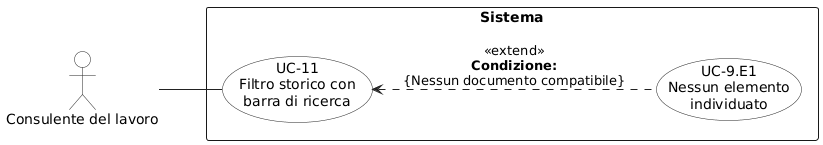
\includegraphics[width=1.1\textwidth]{diagrammi_use_case/uc_11.png}
    \caption{Diagramma del caso d'uso UC-11: Filtro storico con barra di ricerca}
    \label{fig:uc-11}
\end{figure}
\begin{description}[style=multiline, leftmargin=4cm, font=\bfseries]
    \item[\glslink{attore}{Attore} Principale] \glslink{consulente-del-lavoro-cdl}{Consulente del lavoro}
    \item[\glslink{trigger}{Trigger}] Il \glslink{consulente-del-lavoro-cdl}{Consulente del lavoro} intende cercare rapidamente documenti nello storico tramite una barra di ricerca unica.
    \item[Pre-condizioni]  Il \glslink{consulente-del-lavoro-cdl}{Consulente del lavoro} si trova nella sezione "Storico documenti analizzati".
    \item[Post-condizioni] Il sistema mostra solo i documenti che corrispondono al testo inserito nella barra di ricerca.
    \item[\glslink{scenario-principale}{Scenario Principale}]
    \begin{enumerate}[leftmargin=*, nosep]
        \item Il \glslink{consulente-del-lavoro-cdl}{Consulente del lavoro} inserisce un testo nella barra di ricerca unica.
        \item Il sistema filtra lo storico confrontando il testo con i campi nome e cognome del dipendente e azienda.
    \end{enumerate}
    \item[Scenari Alternativi]
    \begin{itemize}[leftmargin=*, nosep]
        \item 2a. Nessun elemento individuato: il sistema non trova documenti compatibili con la ricerca; viene eseguito UC-9.E1.
    \end{itemize}
    \item[Relazioni]
    \begin{itemize}[leftmargin=*, nosep]
        \item \textbf{Estensioni}: UC-9.E1.
    \end{itemize}
\end{description}

\subsubsection{UC-12: Filtro storico per stato invio}
\mbox{} \\

\begin{figure}[H]
    \centering
    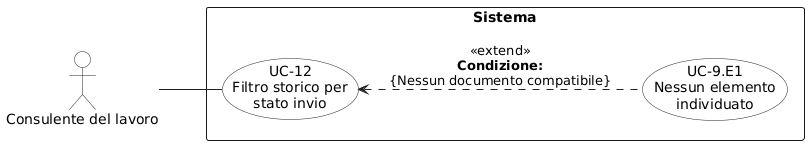
\includegraphics[width=1.1\textwidth]{diagrammi_use_case/uc_12.png}
    \caption{Diagramma del caso d'uso UC-12: Filtro storico per stato invio}
    \label{fig:uc-12}
\end{figure}
\begin{description}[style=multiline, leftmargin=4cm, font=\bfseries]
    \item[\glslink{attore}{Attore} Principale] \glslink{consulente-del-lavoro-cdl}{Consulente del lavoro}
    \item[\glslink{trigger}{Trigger}] Il \glslink{consulente-del-lavoro-cdl}{Consulente del lavoro} intende visualizzare solo documenti inviati o non inviati.
    \item[Pre-condizioni] Il \glslink{consulente-del-lavoro-cdl}{Consulente del lavoro} si trova nella sezione "Storico documenti analizzati".
    \item[Post-condizioni] Il sistema mostra solo i documenti che rispettano lo stato invio selezionato.
    \item[\glslink{scenario-principale}{Scenario Principale}]
    \begin{enumerate}[leftmargin=*, nosep]
        \item Il \glslink{consulente-del-lavoro-cdl}{Consulente del lavoro} seleziona il filtro di stato invio scegliendo tra "Inviato" e "Non inviato".
        \item Il sistema aggiorna la lista mostrando i documenti coerenti con lo stato selezionato.
    \end{enumerate}
    \item[Scenari Alternativi]
    \begin{itemize}[leftmargin=*, nosep]
        \item 2a. Nessun elemento individuato: il sistema non trova documenti compatibili con il filtro selezionato; viene eseguito UC-9.E1.
    \end{itemize}
    \item[Relazioni]
    \begin{itemize}[leftmargin=*, nosep]
        \item \textbf{Estensioni}: UC-9.E1.
    \end{itemize}
\end{description}

\subsubsection{UC-13: Filtro storico per confidenza}
\mbox{} \\

\begin{figure}[H]
    \centering
    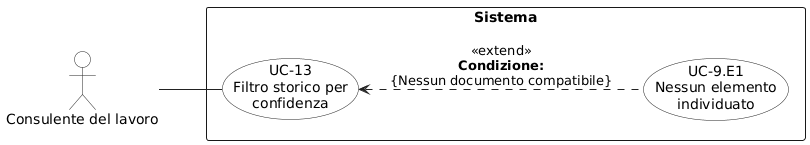
\includegraphics[width=1.1\textwidth]{diagrammi_use_case/uc_13.png}
    \caption{Diagramma del caso d'uso UC-13: Filtro storico per confidenza}
    \label{fig:uc-13}
\end{figure}
\begin{description}[style=multiline, leftmargin=4cm, font=\bfseries]
    \item[\glslink{attore}{Attore} Principale] \glslink{consulente-del-lavoro-cdl}{Consulente del lavoro}
    \item[\glslink{trigger}{Trigger}] Il \glslink{consulente-del-lavoro-cdl}{Consulente del lavoro} intende filtrare lo storico in base alla \glslink{confidenza-confidence-score}{confidenza} dei dati estratti rispetto a una soglia.
    \item[Pre-condizioni] Il \glslink{consulente-del-lavoro-cdl}{Consulente del lavoro} si trova nella sezione "Storico documenti analizzati".
    \item[Post-condizioni] Il sistema mostra solo i documenti con \glslink{confidenza-confidence-score}{confidenza} maggiore o minore della soglia impostata.
    \item[\glslink{scenario-principale}{Scenario Principale}]
    \begin{enumerate}[leftmargin=*, nosep]
        \item Il \glslink{consulente-del-lavoro-cdl}{Consulente del lavoro} imposta una \glslink{soglia-di-confidenza}{soglia di confidenza} e seleziona il criterio (maggiore di soglia o minore di soglia).
        \item Il sistema aggiorna la lista mostrando i documenti che rispettano il criterio scelto.
    \end{enumerate}
    \item[Scenari Alternativi]
    \begin{itemize}[leftmargin=*, nosep]
        \item 2a. Nessun elemento individuato: il sistema non trova documenti compatibili con il filtro impostato; viene eseguito UC-9.E1.
    \end{itemize}
    \item[Relazioni]
    \begin{itemize}[leftmargin=*, nosep]
        \item \textbf{Estensioni}: UC-9.E1.
    \end{itemize}
\end{description}

\subsubsection{UC-14: Filtro storico per mese e anno}
\mbox{} \\

\begin{figure}[H]
    \centering
    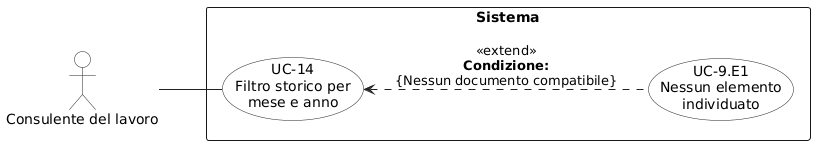
\includegraphics[width=1.1\textwidth]{diagrammi_use_case/uc_14.png}
    \caption{Diagramma del caso d'uso UC-14: Filtro storico per mese e anno}
    \label{fig:uc-14}
\end{figure}
\begin{description}[style=multiline, leftmargin=4cm, font=\bfseries]
    \item[\glslink{attore}{Attore} Principale] \glslink{consulente-del-lavoro-cdl}{Consulente del lavoro}
    \item[\glslink{trigger}{Trigger}] Il \glslink{consulente-del-lavoro-cdl}{Consulente del lavoro} intende visualizzare i documenti relativi a uno specifico mese e anno.
    \item[Pre-condizioni]  Il \glslink{consulente-del-lavoro-cdl}{Consulente del lavoro} si trova nella sezione "Storico documenti analizzati".
    \item[Post-condizioni] Il sistema mostra solo i documenti riferiti al mese e all'anno selezionati.
    \item[\glslink{scenario-principale}{Scenario Principale}]
    \begin{enumerate}[leftmargin=*, nosep]
        \item Il \glslink{consulente-del-lavoro-cdl}{Consulente del lavoro} seleziona mese e anno nel filtro temporale.
        \item Il sistema aggiorna la lista mostrando i documenti compatibili con il periodo selezionato.
    \end{enumerate}
    \item[Scenari Alternativi]
    \begin{itemize}[leftmargin=*, nosep]
        \item 2a. Nessun elemento individuato: il sistema non trova documenti compatibili con il periodo selezionato; viene eseguito UC-9.E1.
    \end{itemize}
    \item[Relazioni]
    \begin{itemize}[leftmargin=*, nosep]
        \item \textbf{Estensioni}: UC-9.E1.
    \end{itemize}
\end{description}
\newpage
\subsubsection{UC-15: Visualizzazione singolo documento dallo storico}
\mbox{} \\

\begin{figure}[H]
    \centering
    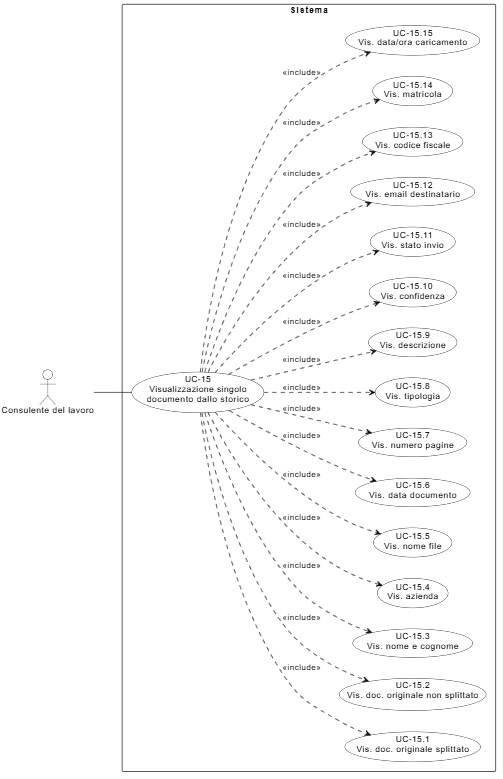
\includegraphics[width=1\textwidth]{diagrammi_use_case/uc_15.png}
    \caption{Diagramma del caso d'uso UC-15: Visualizzazione singolo documento dallo storico}
    \label{fig:uc-15}
\end{figure}
\begin{description}[style=multiline, leftmargin=4cm, font=\bfseries]
    \item[\glslink{attore}{Attore} Principale] \glslink{consulente-del-lavoro-cdl}{Consulente del lavoro}
    \item[\glslink{trigger}{Trigger}] Il \glslink{consulente-del-lavoro-cdl}{Consulente del lavoro} intende consultare il dettaglio di un documento selezionato dallo storico.
    \item[Pre-condizioni] Lo storico contiene almeno un documento e il \glslink{consulente-del-lavoro-cdl}{Consulente del lavoro} ha selezionato una riga della lista.
    \item[Post-condizioni] Il sistema mostra il dettaglio del documento selezionato.
    \item[\glslink{scenario-principale}{Scenario Principale}]
    \begin{enumerate}[leftmargin=*, nosep]
        \item Il \glslink{consulente-del-lavoro-cdl}{Consulente del lavoro} seleziona un documento dall'elenco dello storico.
        \item Il sistema apre la vista di dettaglio con layout affiancato: documento originale a sinistra e dati estratti a destra.
        \item Il sistema mostra il documento originale splittato relativo al dipendente selezionato (\textbf{UC-15.1}).
        \item Il sistema mostra il documento originale non splittato (\textbf{UC-15.2}).
        \item Il sistema mostra i campi estratti del documento: nome e cognome del dipendente (\textbf{UC-15.3}), azienda (\textbf{UC-15.4}), nome del file (\textbf{UC-15.5}), data del documento (\textbf{UC-15.6}), numero di pagine (\textbf{UC-15.7}), tipologia del documento (\textbf{UC-15.8}), breve descrizione del documento (\textbf{UC-15.9}), \glslink{confidenza-confidence-score}{confidenza} in percentuale (\textbf{UC-15.10}), stato di invio del documento (\textbf{UC-15.11}), email destinatario (\textbf{UC-15.12}), codice fiscale (\textbf{UC-15.13}), matricola dipendente (\textbf{UC-15.14}) e data/ora caricamento (\textbf{UC-15.15}).
    \end{enumerate}
    \item[Relazioni]
    \begin{itemize}[leftmargin=*, nosep]
        \item \textbf{Inclusioni}: UC-15.1, UC-15.2, UC-15.3, UC-15.4, UC-15.5, UC-15.6, UC-15.7, UC-15.8, UC-15.9, UC-15.10, UC-15.11, UC-15.12, UC-15.13, UC-15.14, UC-15.15.
    \end{itemize}
\end{description}

\paragraph{UC-15.1: Visualizzazione documento originale splittato}
\mbox{} \\

\begin{figure}[H]
    \centering
    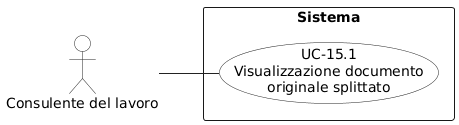
\includegraphics[width=0.7\textwidth]{diagrammi_use_case/uc_15.1.png}
    \caption{Diagramma del caso d'uso UC-15.1: Visualizzazione documento originale splittato}
    \label{fig:uc-15.1}
\end{figure}
\begin{description}[style=multiline, leftmargin=4cm, font=\bfseries]
    \item[\glslink{attore}{Attore} Principale] \glslink{consulente-del-lavoro-cdl}{Consulente del lavoro}
    \item[Pre-condizioni] Il \glslink{consulente-del-lavoro-cdl}{Consulente del lavoro} ha aperto il dettaglio di un documento dallo storico (UC-15).
    \item[Post-condizioni] Il sistema mostra la preview del documento originale splittato (parte relativa a un singolo dipendente) nel pannello sinistro della vista di dettaglio.
    \item[\glslink{scenario-principale}{Scenario Principale}]
    \begin{enumerate}[leftmargin=*, nosep]
        \item Il sistema carica la porzione splittata del file originale associata al dipendente selezionato.
        \item Il sistema visualizza il documento in anteprima nel pannello dedicato.
    \end{enumerate}
\end{description}

\paragraph{UC-15.2: Visualizzazione documento originale non splittato}
\mbox{} \\

\begin{figure}[H]
    \centering
    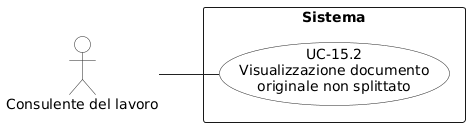
\includegraphics[width=0.7\textwidth]{diagrammi_use_case/uc_15.2.png}
    \caption{Diagramma del caso d'uso UC-15.2: Visualizzazione documento originale non splittato}
    \label{fig:uc-15.2}
\end{figure}
\begin{description}[style=multiline, leftmargin=4cm, font=\bfseries]
    \item[\glslink{attore}{Attore} Principale] \glslink{consulente-del-lavoro-cdl}{Consulente del lavoro}
    \item[Pre-condizioni] Il \glslink{consulente-del-lavoro-cdl}{Consulente del lavoro} ha aperto il dettaglio di un documento dallo storico (UC-15).
    \item[Post-condizioni] Il sistema mostra la preview del documento originale completo (non splittato) nel pannello sinistro della vista di dettaglio.
    \item[\glslink{scenario-principale}{Scenario Principale}]
    \begin{enumerate}[leftmargin=*, nosep]
        \item Il sistema carica il file originale completo associato al record selezionato.
        \item Il sistema visualizza il documento in anteprima nel pannello dedicato.
    \end{enumerate}
\end{description}

\paragraph{UC-15.3: Visualizzazione nome e cognome del dipendente}
\mbox{} \\

\begin{figure}[H]
    \centering
    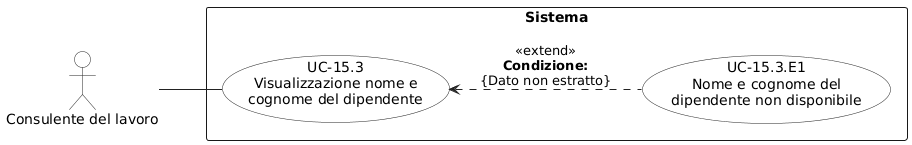
\includegraphics[width=1.1\textwidth]{diagrammi_use_case/uc_15.3.png}
    \caption{Diagramma del caso d'uso UC-15.3: Visualizzazione nome e cognome del dipendente}
    \label{fig:uc-15.3}
\end{figure}
\begin{description}[style=multiline, leftmargin=4cm, font=\bfseries]
    \item[\glslink{attore}{Attore} Principale] \glslink{consulente-del-lavoro-cdl}{Consulente del lavoro}
    \item[Pre-condizioni] Il sistema ha estratto i dati dal documento selezionato.
    \item[Post-condizioni] Il sistema mostra il valore del campo nome e cognome del dipendente.
    \item[\glslink{scenario-principale}{Scenario Principale}]
    \begin{enumerate}[leftmargin=*, nosep]
        \item Il sistema visualizza nel pannello dati estratti il nome e cognome del dipendente associato al documento.
    \end{enumerate}
    \item[Scenari Alternativi]
    \begin{itemize}[leftmargin=*, nosep]
        \item 1a. Nome e cognome non disponibile: il sistema non dispone del dato estratto; viene eseguito UC-15.3.E1.
    \end{itemize}
    \item[Relazioni]
    \begin{itemize}[leftmargin=*, nosep]
        \item \textbf{Estensioni}: UC-15.3.E1.
    \end{itemize}
\end{description}

\paragraph{UC-15.4: Visualizzazione azienda}
\mbox{} \\

\begin{figure}[H]
    \centering
    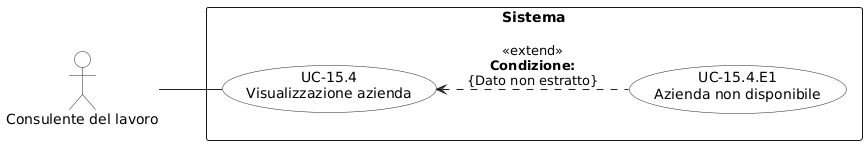
\includegraphics[width=1.1\textwidth]{diagrammi_use_case/uc_15.4.png}
    \caption{Diagramma del caso d'uso UC-15.4: Visualizzazione azienda}
    \label{fig:uc-15.4}
\end{figure}
\begin{description}[style=multiline, leftmargin=4cm, font=\bfseries]
    \item[\glslink{attore}{Attore} Principale] \glslink{consulente-del-lavoro-cdl}{Consulente del lavoro}
    \item[Pre-condizioni] Il sistema ha estratto i dati dal documento selezionato.
    \item[Post-condizioni] Il sistema mostra il valore del campo azienda.
    \item[\glslink{scenario-principale}{Scenario Principale}]
    \begin{enumerate}[leftmargin=*, nosep]
        \item Il sistema visualizza nel pannello dati estratti l'azienda associata al documento.
    \end{enumerate}
    \item[Scenari Alternativi]
    \begin{itemize}[leftmargin=*, nosep]
        \item 1a. Azienda non disponibile: il sistema non dispone del dato estratto; viene eseguito UC-15.4.E1.
    \end{itemize}
    \item[Relazioni]
    \begin{itemize}[leftmargin=*, nosep]
        \item \textbf{Estensioni}: UC-15.4.E1.
    \end{itemize}
\end{description}
\newpage
\paragraph{UC-15.5: Visualizzazione nome del file}
\mbox{} \\

\begin{figure}[H]
    \centering
    
\includegraphics[width=0.7\textwidth]{diagrammi_use_case/uc_15.5.png}
    \caption{Diagramma del caso d'uso UC-15.5: Visualizzazione nome del file}
    \label{fig:uc-15.5}
\end{figure}
\begin{description}[style=multiline, leftmargin=4cm, font=\bfseries]
    \item[\glslink{attore}{Attore} Principale] \glslink{consulente-del-lavoro-cdl}{Consulente del lavoro}
    \item[Pre-condizioni] Il sistema ha estratto i dati dal documento selezionato.
    \item[Post-condizioni] Il sistema mostra il valore del campo nome del file.
    \item[\glslink{scenario-principale}{Scenario Principale}]
    \begin{enumerate}[leftmargin=*, nosep]
        \item Il sistema visualizza nel pannello dati estratti il nome del file del documento.
    \end{enumerate}
\end{description}

\paragraph{UC-15.6: Visualizzazione data del documento}
\mbox{} \\

\begin{figure}[H]
    \centering
    
\includegraphics[width=1.1\textwidth]{diagrammi_use_case/uc_15.6.png}
    \caption{Diagramma del caso d'uso UC-15.6: Visualizzazione data del documento}
    \label{fig:uc-15.6}
\end{figure}
\begin{description}[style=multiline, leftmargin=4cm, font=\bfseries]
    \item[\glslink{attore}{Attore} Principale] \glslink{consulente-del-lavoro-cdl}{Consulente del lavoro}
    \item[Pre-condizioni] Il sistema ha estratto i dati dal documento selezionato.
    \item[Post-condizioni] Il sistema mostra il valore del campo data del documento.
    \item[\glslink{scenario-principale}{Scenario Principale}]
    \begin{enumerate}[leftmargin=*, nosep]
        \item Il sistema visualizza nel pannello dati estratti la data del documento.
    \end{enumerate}
    \item[Scenari Alternativi]
    \begin{itemize}[leftmargin=*, nosep]
        \item 1a. Data del documento non disponibile: il sistema non dispone del dato estratto; viene eseguito UC-15.6.E1.
    \end{itemize}
    \item[Relazioni]
    \begin{itemize}[leftmargin=*, nosep]
        \item \textbf{Estensioni}: UC-15.6.E1.
    \end{itemize}
\end{description}

\paragraph{UC-15.7: Visualizzazione numero di pagine}
\mbox{} \\

\begin{figure}[H]
    \centering
    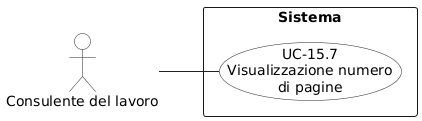
\includegraphics[width=0.65\textwidth]{diagrammi_use_case/uc_15.7.png}
    \caption{Diagramma del caso d'uso UC-15.7: Visualizzazione numero di pagine}
    \label{fig:uc-15.7}
\end{figure}
\begin{description}[style=multiline, leftmargin=4cm, font=\bfseries]
    \item[\glslink{attore}{Attore} Principale] \glslink{consulente-del-lavoro-cdl}{Consulente del lavoro}
    \item[Pre-condizioni] Il sistema ha estratto i dati dal documento selezionato.
    \item[Post-condizioni] Il sistema mostra il valore del campo numero di pagine.
    \item[\glslink{scenario-principale}{Scenario Principale}]
    \begin{enumerate}[leftmargin=*, nosep]
        \item Il sistema visualizza nel pannello dati estratti il numero di pagine del documento.
    \end{enumerate}
\end{description}

\paragraph{UC-15.8: Visualizzazione tipologia del documento}
\mbox{} \\

\begin{figure}[H]
    \centering
    
\includegraphics[width=1.1\textwidth]{diagrammi_use_case/uc_15.8.png}
    \caption{Diagramma del caso d'uso UC-15.8: Visualizzazione tipologia del documento}
    \label{fig:uc-15.8}
\end{figure}
\begin{description}[style=multiline, leftmargin=4cm, font=\bfseries]
    \item[\glslink{attore}{Attore} Principale] \glslink{consulente-del-lavoro-cdl}{Consulente del lavoro}
    \item[Pre-condizioni] Il sistema ha estratto i dati dal documento selezionato.
    \item[Post-condizioni] Il sistema mostra il valore del campo tipologia del documento.
    \item[\glslink{scenario-principale}{Scenario Principale}]
    \begin{enumerate}[leftmargin=*, nosep]
        \item Il sistema visualizza nel pannello dati estratti la tipologia del documento.
    \end{enumerate}
    \item[Scenari Alternativi]
    \begin{itemize}[leftmargin=*, nosep]
        \item 1a. Tipologia del documento non disponibile: il sistema non dispone del dato estratto; viene eseguito UC-15.8.E1.
    \end{itemize}
    \item[Relazioni]
    \begin{itemize}[leftmargin=*, nosep]
        \item \textbf{Estensioni}: UC-15.8.E1.
    \end{itemize}
\end{description}

\paragraph{UC-15.9: Visualizzazione breve descrizione del documento}
\mbox{} \\

\begin{figure}[H]
    \centering
    
\includegraphics[width=1.1\textwidth]{diagrammi_use_case/uc_15.9.png}
    \caption{Diagramma del caso d'uso UC-15.9: Visualizzazione breve descrizione del documento}
    \label{fig:uc-15.9}
\end{figure}
\begin{description}[style=multiline, leftmargin=4cm, font=\bfseries]
    \item[\glslink{attore}{Attore} Principale] \glslink{consulente-del-lavoro-cdl}{Consulente del lavoro}
    \item[Pre-condizioni] Il sistema ha estratto i dati dal documento selezionato.
    \item[Post-condizioni] Il sistema mostra il valore del campo breve descrizione del documento.
    \item[\glslink{scenario-principale}{Scenario Principale}]
    \begin{enumerate}[leftmargin=*, nosep]
        \item Il sistema visualizza nel pannello dati estratti la breve descrizione del documento.
    \end{enumerate}
    \item[Scenari Alternativi]
    \begin{itemize}[leftmargin=*, nosep]
        \item 1a. Breve descrizione non disponibile: il sistema non dispone del dato estratto; viene eseguito UC-15.9.E1.
    \end{itemize}
    \item[Relazioni]
    \begin{itemize}[leftmargin=*, nosep]
        \item \textbf{Estensioni}: UC-15.9.E1.
    \end{itemize}
\end{description}

\paragraph{UC-15.10: Visualizzazione confidenza in percentuale per documento}
\mbox{} \\

\begin{figure}[H]
    \centering
    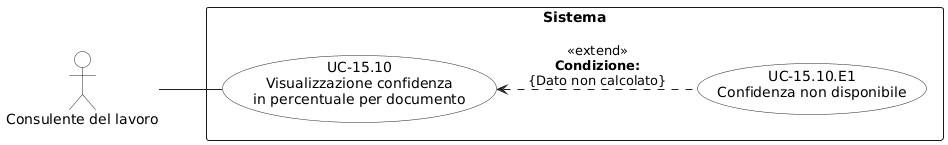
\includegraphics[width=1.1\textwidth]{diagrammi_use_case/uc_15.10.png}
    \caption{Diagramma del caso d'uso UC-15.10: Visualizzazione confidenza in percentuale per documento}
    \label{fig:uc-15.10}
\end{figure}
\begin{description}[style=multiline, leftmargin=4cm, font=\bfseries]
    \item[\glslink{attore}{Attore} Principale] \glslink{consulente-del-lavoro-cdl}{Consulente del lavoro}
    \item[Pre-condizioni] Il sistema ha estratto i dati dal documento selezionato.
    \item[Post-condizioni] Il sistema mostra il valore del campo \glslink{confidenza-confidence-score}{confidenza} in percentuale.
    \item[\glslink{scenario-principale}{Scenario Principale}]
    \begin{enumerate}[leftmargin=*, nosep]
        \item Il sistema visualizza nel pannello dati estratti la \glslink{confidenza-confidence-score}{confidenza} in percentuale (da 0 a 100\%) che indica l'affidabilità dei dati estratti dall'\glslink{intelligenza-artificiale-ai}{AI} per il documento analizzato.
    \end{enumerate}
    \item[Scenari Alternativi]
    \begin{itemize}[leftmargin=*, nosep]
        \item 1a. \glslink{confidenza-confidence-score}{Confidenza} non disponibile: il sistema non dispone del dato estratto; viene eseguito UC-15.10.E1.
    \end{itemize}
    \item[Relazioni]
    \begin{itemize}[leftmargin=*, nosep]
        \item \textbf{Estensioni}: UC-15.10.E1.
    \end{itemize}
\end{description}

\paragraph{UC-15.11: Visualizzazione stato invio documento}
\mbox{} \\

\begin{figure}[H]
    \centering
    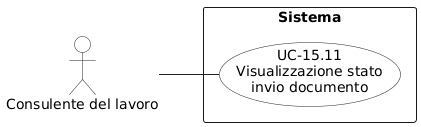
\includegraphics[width=0.65\textwidth]{diagrammi_use_case/uc_15.11.png}
    \caption{Diagramma del caso d'uso UC-15.11: Visualizzazione stato invio documento}
    \label{fig:uc-15.11}
\end{figure}
\begin{description}[style=multiline, leftmargin=4cm, font=\bfseries]
    \item[\glslink{attore}{Attore} Principale] \glslink{consulente-del-lavoro-cdl}{Consulente del lavoro}
    \item[Pre-condizioni] Il sistema dispone delle informazioni di stato invio del documento selezionato.
    \item[Post-condizioni] Il sistema mostra se il documento è stato inviato oppure no.
    \item[\glslink{scenario-principale}{Scenario Principale}]
    \begin{enumerate}[leftmargin=*, nosep]
        \item Il sistema visualizza nel pannello dati estratti lo stato di invio del documento con un valore tra "Inviato" e "Non inviato".
    \end{enumerate}
\end{description}

\paragraph{UC-15.12: Visualizzazione email destinatario}
\mbox{} \\
\begin{figure}[H]
    \centering
    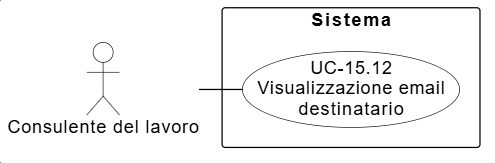
\includegraphics[width=0.6\textwidth]{diagrammi_use_case/uc_15.12.png}
    \caption{Diagramma del caso d'uso UC-15.12: Visualizzazione email destinatario}
    \label{fig:uc-15.12}
\end{figure}
\begin{description}[style=multiline, leftmargin=4cm, font=\bfseries]
    \item[\glslink{attore}{Attore} Principale] \glslink{consulente-del-lavoro-cdl}{Consulente del lavoro}
    \item[Pre-condizioni] Il sistema ha eseguito l'estrazione dei \glslink{metadati}{metadati} dal documento selezionato.
    \item[Post-condizioni] Il sistema mostra il valore del campo email del destinatario nel pannello dati estratti.
    \item[\glslink{scenario-principale}{Scenario Principale}]
    \begin{enumerate}[leftmargin=*, nosep]
        \item Il sistema recupera l'indirizzo e-mail estratto associato al documento.
        \item Il sistema visualizza l'indirizzo e-mail nel pannello dati estratti con eventuale icona per copiarlo o inviare una mail rapida.
    \end{enumerate}
\end{description}


\paragraph{UC-15.13: Visualizzazione codice fiscale}
\mbox{} \\
\begin{figure}[H]
    \centering
    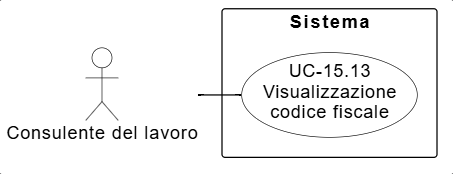
\includegraphics[width=0.6\textwidth]{diagrammi_use_case/uc_15.13.png}
    \caption{Diagramma del caso d'uso UC-15.13: Visualizzazione codice fiscale}
    \label{fig:uc-15.13}
\end{figure}
\begin{description}[style=multiline, leftmargin=4cm, font=\bfseries]
    \item[\glslink{attore}{Attore} Principale] \glslink{consulente-del-lavoro-cdl}{Consulente del lavoro}
    \item[Pre-condizioni] Il sistema ha estratto i \glslink{metadati}{metadati} anagrafici dal documento.
    \item[Post-condizioni] Il sistema mostra il codice fiscale del dipendente nel pannello dati estratti.
    \item[\glslink{scenario-principale}{Scenario Principale}]
    \begin{enumerate}[leftmargin=*, nosep]
        \item Il sistema recupera il codice fiscale estratto.
    \   \item Il sistema visualizza il codice fiscale con un controllo di validità formale (checksum).
\end{enumerate}
\end{description}

\paragraph{UC-15.14: Visualizzazione matricola dipendente}
\mbox{} \\
\begin{figure}[H]
    \centering
    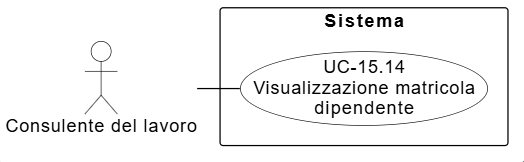
\includegraphics[width=0.6\textwidth]{diagrammi_use_case/uc_15.14.png}
    \caption{Diagramma del caso d'uso UC-15.14: Visualizzazione matricola dipendente}
    \label{fig:uc-15.14}
    \end{figure}
\begin{description}[style=multiline, leftmargin=4cm, font=\bfseries]
    \item[\glslink{attore}{Attore} Principale] \glslink{consulente-del-lavoro-cdl}{Consulente del lavoro}
    \item[Pre-condizioni] Il sistema ha estratto o associato l'identificativo interno (matricola) al documento.
    \item[Post-condizioni] Il sistema mostra la matricola del dipendente nel pannello dati estratti.
    \item[\glslink{scenario-principale}{Scenario Principale}]
    \begin{enumerate}[leftmargin=*, nosep]
       \item Il sistema recupera la matricola associata al record.
       \item Il sistema visualizza la matricola e fornisce link/azione per consultare la scheda dipendente correlata.
    \end{enumerate}
\end{description}

\paragraph{UC-15.15: Visualizzazione data/ora caricamento}
\mbox{} \\
\begin{figure}[H]
    \centering
    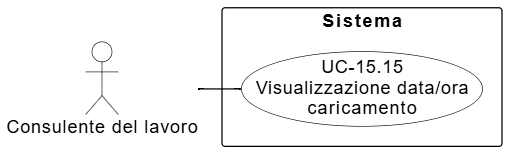
\includegraphics[width=0.6\textwidth]{diagrammi_use_case/uc_15.15.png}
    \caption{Diagramma del caso d'uso UC-15.15: Visualizzazione data/ora caricamento}
    \label{fig:uc-15.15}
\end{figure}
\begin{description}[style=multiline, leftmargin=4cm, font=\bfseries]
    \item[\glslink{attore}{Attore} Principale] \glslink{consulente-del-lavoro-cdl}{Consulente del lavoro}
    \item[Pre-condizioni] Il record del documento contiene il timestamp di caricamento.
    \item[Post-condizioni] Il sistema mostra la data e l'ora di caricamento del documento nello storico.
    \item[\glslink{scenario-principale}{Scenario Principale}]
    \begin{enumerate}[leftmargin=*, nosep]
        \item Il sistema legge il timestamp di caricamento associato al documento.
        \item Il sistema visualizza la data/ora nel pannello dati estratti e nel sommario dello storico.
\end{enumerate}
\end{description}

\paragraph{UC-15.3.E1: Nome e cognome del dipendente non disponibile}
\mbox{} \\

\begin{figure}[H]
    \centering
    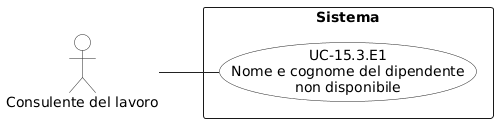
\includegraphics[width=0.75\textwidth]{diagrammi_use_case/uc_15.3.E1.png}
    \caption{Diagramma del caso d'uso UC-15.3.E1: Nome e cognome del dipendente non disponibile}
    \label{fig:uc-15.3.e1}
\end{figure}
\begin{description}[style=multiline, leftmargin=4cm, font=\bfseries]
    \item[\glslink{attore}{Attore} Principale] \glslink{consulente-del-lavoro-cdl}{Consulente del lavoro}
    \item[Pre-condizioni] Il \glslink{consulente-del-lavoro-cdl}{Consulente del lavoro} sta visualizzando il campo nome e cognome del dipendente (UC-15.3) e il dato non è disponibile.
    \item[Post-condizioni] Il sistema mantiene aperta la vista di dettaglio e segnala che il campo nome e cognome del dipendente non è valorizzato.
    \item[\glslink{scenario-principale}{Scenario Principale}]
    \begin{enumerate}[leftmargin=*, nosep]
        \item Il sistema rileva che il campo nome e cognome del dipendente non è disponibile.
        \item Il sistema visualizza il valore "Non disponibile" in corrispondenza del campo.
    \end{enumerate}
\end{description}

\paragraph{UC-15.4.E1: Azienda non disponibile}
\mbox{} \\

\begin{figure}[H]
    \centering
    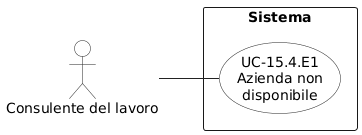
\includegraphics[width=0.6\textwidth]{diagrammi_use_case/uc_15.4.E1.png}
    \caption{Diagramma del caso d'uso UC-15.4.E1: Azienda non disponibile}
    \label{fig:uc-15.4.e1}
\end{figure}
\begin{description}[style=multiline, leftmargin=4cm, font=\bfseries]
    \item[\glslink{attore}{Attore} Principale] \glslink{consulente-del-lavoro-cdl}{Consulente del lavoro}
    \item[Pre-condizioni] Il \glslink{consulente-del-lavoro-cdl}{Consulente del lavoro} sta visualizzando il campo azienda (UC-15.4) e il dato non è disponibile.
    \item[Post-condizioni] Il sistema mantiene aperta la vista di dettaglio e segnala che il campo azienda non è valorizzato.
    \item[\glslink{scenario-principale}{Scenario Principale}]
    \begin{enumerate}[leftmargin=*, nosep]
        \item Il sistema rileva che il campo azienda non è disponibile.
        \item Il sistema visualizza il valore "Non disponibile" in corrispondenza del campo.
    \end{enumerate}
\end{description}

\paragraph{UC-15.6.E1: Data del documento non disponibile}
\mbox{} \\

\begin{figure}[H]
    \centering
    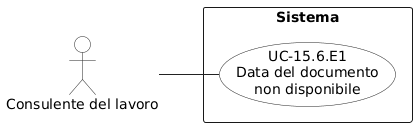
\includegraphics[width=0.7\textwidth]{diagrammi_use_case/uc_15.6.E1.png}
    \caption{Diagramma del caso d'uso UC-15.6.E1: Data del documento non disponibile}
    \label{fig:uc-15.6.e1}
\end{figure}
\begin{description}[style=multiline, leftmargin=4cm, font=\bfseries]
    \item[\glslink{attore}{Attore} Principale] \glslink{consulente-del-lavoro-cdl}{Consulente del lavoro}
    \item[Pre-condizioni] Il \glslink{consulente-del-lavoro-cdl}{Consulente del lavoro} sta visualizzando il campo data del documento (UC-15.6) e il dato non è disponibile.
    \item[Post-condizioni] Il sistema mantiene aperta la vista di dettaglio e segnala che il campo data del documento non è valorizzato.
    \item[\glslink{scenario-principale}{Scenario Principale}]
    \begin{enumerate}[leftmargin=*, nosep]
        \item Il sistema rileva che il campo data del documento non è disponibile.
        \item Il sistema visualizza il valore "Non disponibile" in corrispondenza del campo.
    \end{enumerate}
\end{description}

\paragraph{UC-15.8.E1: Tipologia del documento non disponibile}
\mbox{} \\

\begin{figure}[H]
    \centering
    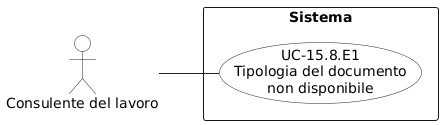
\includegraphics[width=0.7\textwidth]{diagrammi_use_case/uc_15.8.E1.png}
    \caption{Diagramma del caso d'uso UC-15.8.E1: Tipologia del documento non disponibile}
    \label{fig:uc-15.8.e1}
\end{figure}
\begin{description}[style=multiline, leftmargin=4cm, font=\bfseries]
    \item[\glslink{attore}{Attore} Principale] \glslink{consulente-del-lavoro-cdl}{Consulente del lavoro}
    \item[Pre-condizioni] Il \glslink{consulente-del-lavoro-cdl}{Consulente del lavoro} sta visualizzando il campo tipologia del documento (UC-15.8) e il dato non è disponibile.
    \item[Post-condizioni] Il sistema mantiene aperta la vista di dettaglio e segnala che il campo tipologia del documento non è valorizzato.
    \item[\glslink{scenario-principale}{Scenario Principale}]
    \begin{enumerate}[leftmargin=*, nosep]
        \item Il sistema rileva che il campo tipologia del documento non è disponibile.
        \item Il sistema visualizza il valore "Non disponibile" in corrispondenza del campo.
    \end{enumerate}
\end{description}

\paragraph{UC-15.9.E1: Breve descrizione del documento non disponibile}
\mbox{} \\

\begin{figure}[H]
    \centering
    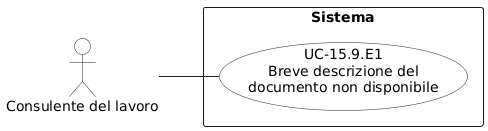
\includegraphics[width=0.7\textwidth]{diagrammi_use_case/uc_15.9.E1.png}
    \caption{Diagramma del caso d'uso UC-15.9.E1: Breve descrizione del documento non disponibile}
    \label{fig:uc-15.9.e1}
\end{figure}
\begin{description}[style=multiline, leftmargin=4cm, font=\bfseries]
    \item[\glslink{attore}{Attore} Principale] \glslink{consulente-del-lavoro-cdl}{Consulente del lavoro}
    \item[Pre-condizioni] Il \glslink{consulente-del-lavoro-cdl}{Consulente del lavoro} sta visualizzando il campo breve descrizione del documento (UC-15.9) e il dato non è disponibile.
    \item[Post-condizioni] Il sistema mantiene aperta la vista di dettaglio e segnala che il campo breve descrizione del documento non è valorizzato.
    \item[\glslink{scenario-principale}{Scenario Principale}]
    \begin{enumerate}[leftmargin=*, nosep]
        \item Il sistema rileva che il campo breve descrizione del documento non è disponibile.
        \item Il sistema visualizza il valore "Non disponibile" in corrispondenza del campo.
    \end{enumerate}
\end{description}

\paragraph{UC-15.10.E1: Confidenza non disponibile}
\mbox{} \\

\begin{figure}[H]
    \centering
    
\includegraphics[width=0.6\textwidth]{diagrammi_use_case/uc_15.10.E1.png}
    \caption{Diagramma del caso d'uso UC-15.10.E1: Confidenza non disponibile}
    \label{fig:uc-15.10.e1}
\end{figure}
\begin{description}[style=multiline, leftmargin=4cm, font=\bfseries]
    \item[\glslink{attore}{Attore} Principale] \glslink{consulente-del-lavoro-cdl}{Consulente del lavoro}
    \item[Pre-condizioni] Il \glslink{consulente-del-lavoro-cdl}{Consulente del lavoro} sta visualizzando il campo \glslink{confidenza-confidence-score}{confidenza} in percentuale (UC-15.10) e il dato non è disponibile.
    \item[Post-condizioni] Il sistema mantiene aperta la vista di dettaglio e segnala che il campo \glslink{confidenza-confidence-score}{confidenza} non è valorizzato.
    \item[\glslink{scenario-principale}{Scenario Principale}]
    \begin{enumerate}[leftmargin=*, nosep]
        \item Il sistema rileva che il campo \glslink{confidenza-confidence-score}{confidenza} non è disponibile.
        \item Il sistema visualizza il valore "Non disponibile" in corrispondenza del campo.
    \end{enumerate}
\end{description}
\newpage
\subsubsection{UC-16: Modifica del singolo documento dallo storico}
\mbox{} \\

\begin{figure}[H]
    \centering
    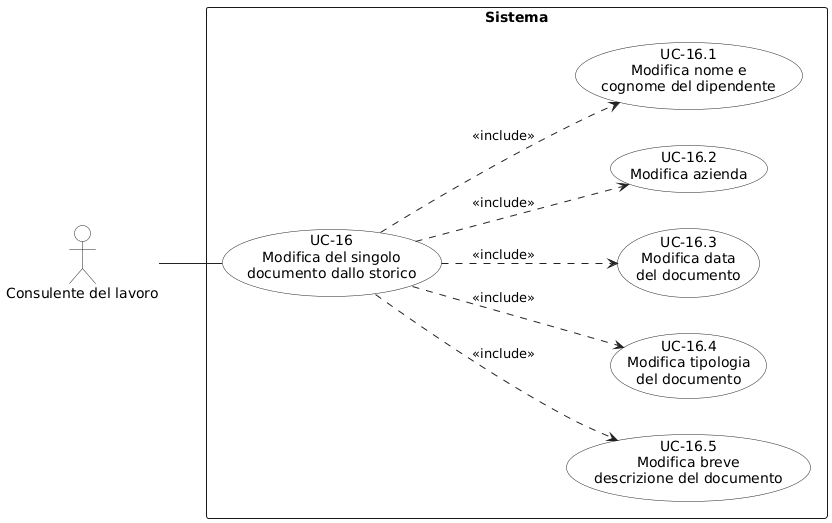
\includegraphics[width=1\textwidth]{diagrammi_use_case/uc_16.png}
    \caption{Diagramma del caso d'uso UC-16: Modifica del singolo documento dallo storico}
    \label{fig:uc-16}
\end{figure}
\begin{description}[style=multiline, leftmargin=4cm, font=\bfseries]
    \item[\glslink{attore}{Attore} Principale] \glslink{consulente-del-lavoro-cdl}{Consulente del lavoro}
    \item[\glslink{trigger}{Trigger}] Il \glslink{consulente-del-lavoro-cdl}{Consulente del lavoro} intende modificare uno o più campi editabili del documento selezionato.
    \item[Pre-condizioni] Il \glslink{consulente-del-lavoro-cdl}{Consulente del lavoro} si trova nella vista di dettaglio del singolo documento (UC-15).
    \item[Post-condizioni] Il sistema salva le modifiche apportate \glslink{intelligenza-artificiale-ai}{ai} campi editabili del documento selezionato.
    \item[\glslink{scenario-principale}{Scenario Principale}]
    \begin{enumerate}[leftmargin=*, nosep]
\item Il \glslink{consulente-del-lavoro-cdl}{Consulente del lavoro} seleziona l'azione di modifica del documento.
        \item Il sistema abilita la modalità di modifica dei campi consentiti.
        \item Il \glslink{consulente-del-lavoro-cdl}{Consulente del lavoro} modifica nome e cognome del dipendente (\textbf{UC-16.1}).
        \item Il \glslink{consulente-del-lavoro-cdl}{Consulente del lavoro} modifica azienda (\textbf{UC-16.2}).
        \item Il \glslink{consulente-del-lavoro-cdl}{Consulente del lavoro} modifica data del documento (\textbf{UC-16.3}).
        \item Il \glslink{consulente-del-lavoro-cdl}{Consulente del lavoro} modifica tipologia del documento (\textbf{UC-16.4}).
        \item Il \glslink{consulente-del-lavoro-cdl}{Consulente del lavoro} modifica breve descrizione del documento (\textbf{UC-16.5}).
        \item Il \glslink{consulente-del-lavoro-cdl}{Consulente del lavoro} modifica email destinatario (\textbf{UC-16.6}).
        \item Il \glslink{consulente-del-lavoro-cdl}{Consulente del lavoro} modifica codice fiscale (\textbf{UC-16.7}).
        \item Il \glslink{consulente-del-lavoro-cdl}{Consulente del lavoro} modifica matricola dipendente (\textbf{UC-16.8}).
        \item Il \glslink{consulente-del-lavoro-cdl}{Consulente del lavoro} conferma il salvataggio.
        \item Il sistema valida i dati inseriti e salva le modifiche.
    \end{enumerate}
    \item[Relazioni]
    \begin{itemize}[leftmargin=*, nosep]
        \item \textbf{Inclusioni}: UC-16.1, UC-16.2, UC-16.3, UC-16.4, UC-16.5, UC-16.6, UC-16.7, UC-16.8.
    \end{itemize}
\end{description}

\paragraph{UC-16.1: Modifica nome e cognome del dipendente}
\mbox{} \\

\begin{figure}[H]
    \centering
    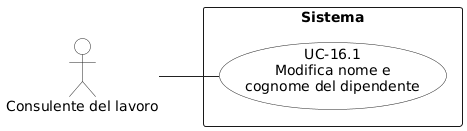
\includegraphics[width=0.75\textwidth]{diagrammi_use_case/uc_16.1.png}
    \caption{Diagramma del caso d'uso UC-16.1: Modifica nome e cognome del dipendente}
    \label{fig:uc-16.1}
\end{figure}
\begin{description}[style=multiline, leftmargin=4cm, font=\bfseries]
    \item[\glslink{attore}{Attore} Principale] \glslink{consulente-del-lavoro-cdl}{Consulente del lavoro}
    \item[Pre-condizioni] Il sistema è in modalità modifica del documento (UC-16).
    \item[Post-condizioni] Il sistema aggiorna il valore del campo nome e cognome del dipendente.
    \item[\glslink{scenario-principale}{Scenario Principale}]
    \begin{enumerate}[leftmargin=*, nosep]
        \item Il \glslink{consulente-del-lavoro-cdl}{Consulente del lavoro} inserisce il nuovo valore nel campo nome e cognome.
        \item Il sistema registra il valore aggiornato in attesa del salvataggio finale.
    \end{enumerate}
\end{description}
\newpage
\paragraph{UC-16.2: Modifica azienda}
\mbox{} \\

\begin{figure}[H]
    \centering
    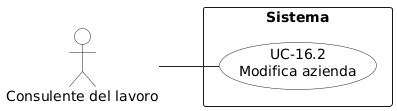
\includegraphics[width=0.65\textwidth]{diagrammi_use_case/uc_16.2.png}
    \caption{Diagramma del caso d'uso UC-16.2: Modifica azienda}
    \label{fig:uc-16.2}
\end{figure}
\begin{description}[style=multiline, leftmargin=4cm, font=\bfseries]
    \item[\glslink{attore}{Attore} Principale] \glslink{consulente-del-lavoro-cdl}{Consulente del lavoro}
    \item[Pre-condizioni] Il sistema è in modalità modifica del documento (UC-16).
    \item[Post-condizioni] Il sistema aggiorna il valore del campo azienda.
    \item[\glslink{scenario-principale}{Scenario Principale}]
    \begin{enumerate}[leftmargin=*, nosep]
        \item Il \glslink{consulente-del-lavoro-cdl}{Consulente del lavoro} inserisce il nuovo valore nel campo azienda.
        \item Il sistema registra il valore aggiornato in attesa del salvataggio finale.
    \end{enumerate}
\end{description}

\paragraph{UC-16.3: Modifica data del documento}
\mbox{} \\

\begin{figure}[H]
    \centering
    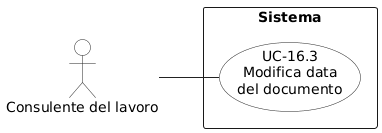
\includegraphics[width=0.65\textwidth]{diagrammi_use_case/uc_16.3.png}
    \caption{Diagramma del caso d'uso UC-16.3: Modifica data del documento}
    \label{fig:uc-16.3}
\end{figure}
\begin{description}[style=multiline, leftmargin=4cm, font=\bfseries]
    \item[\glslink{attore}{Attore} Principale] \glslink{consulente-del-lavoro-cdl}{Consulente del lavoro}
    \item[Pre-condizioni] Il sistema è in modalità modifica del documento (UC-16).
    \item[Post-condizioni] Il sistema aggiorna il valore del campo data del documento.
    \item[\glslink{scenario-principale}{Scenario Principale}]
    \begin{enumerate}[leftmargin=*, nosep]
        \item Il \glslink{consulente-del-lavoro-cdl}{Consulente del lavoro} inserisce o seleziona il nuovo valore nel campo data del documento.
        \item Il sistema registra il valore aggiornato in attesa del salvataggio finale.
    \end{enumerate}
\end{description}

\paragraph{UC-16.4: Modifica tipologia del documento}
\mbox{} \\

\begin{figure}[H]
    \centering
    
\includegraphics[width=0.65\textwidth]{diagrammi_use_case/uc_16.4.png}
    \caption{Diagramma del caso d'uso UC-16.4: Modifica tipologia del documento}
    \label{fig:uc-16.4}
    \end{figure}
\begin{description}[style=multiline, leftmargin=4cm, font=\bfseries]
    \item[\glslink{attore}{Attore} Principale] \glslink{consulente-del-lavoro-cdl}{Consulente del lavoro}
    \item[Pre-condizioni] Il sistema è in modalità modifica del documento (UC-16).
    \item[Post-condizioni] Il sistema aggiorna il valore del campo tipologia del documento.
    \item[\glslink{scenario-principale}{Scenario Principale}]
    \begin{enumerate}[leftmargin=*, nosep]
        \item Il \glslink{consulente-del-lavoro-cdl}{Consulente del lavoro} seleziona il nuovo valore nel campo tipologia del documento tra le opzioni disponibili: cedolino, CU, comunicazione, documento da firmare, lettera, altro.
        \item Il sistema registra il valore aggiornato in attesa del salvataggio finale.
    \end{enumerate}
\end{description}

\paragraph{UC-16.5: Modifica breve descrizione del documento}
\mbox{} \\

\begin{figure}[H]
    \centering
    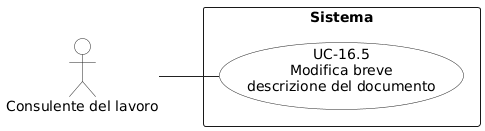
\includegraphics[width=0.75\textwidth]{diagrammi_use_case/uc_16.5.png}
    \caption{Diagramma del caso d'uso UC-16.5: Modifica breve descrizione del documento}
    \label{fig:uc-16.5}
\end{figure}
\begin{description}[style=multiline, leftmargin=4cm, font=\bfseries]
    \item[\glslink{attore}{Attore} Principale] \glslink{consulente-del-lavoro-cdl}{Consulente del lavoro}
    \item[Pre-condizioni] Il sistema è in modalità modifica del documento (UC-16).
    \item[Post-condizioni] Il sistema aggiorna il valore del campo breve descrizione del documento.
    \item[\glslink{scenario-principale}{Scenario Principale}]
    \begin{enumerate}[leftmargin=*, nosep]
        \item Il \glslink{consulente-del-lavoro-cdl}{Consulente del lavoro} inserisce il nuovo valore nel campo breve descrizione del documento.
        \item Il sistema registra il valore aggiornato in attesa del salvataggio finale.
    \end{enumerate}
\end{description}

\paragraph{UC-16.6: Modifica email destinatario}
\mbox{} \\

\begin{figure}[H]
    \centering
    
\includegraphics[width=1\textwidth]{diagrammi_use_case/uc_16.6.png}
    \caption{Diagramma del caso d'uso UC-16.6: Modifica email destinatario}
    \label{fig:uc-16.6}
\end{figure}
\begin{description}[style=multiline, leftmargin=4cm, font=\bfseries]
    \item[\glslink{attore}{Attore} Principale] \glslink{consulente-del-lavoro-cdl}{Consulente del lavoro}
    \item[Pre-condizioni] Il sistema è in modalità modifica del documento (UC-16) e il campo email è visibile nel pannello dati estratti.
    \item[Post-condizioni] Il sistema aggiorna il valore del campo email destinatario e lo registra in attesa del salvataggio finale.
    \item[\glslink{scenario-principale}{Scenario Principale}]
    \begin{enumerate}[leftmargin=*, nosep]
        \item Il \glslink{consulente-del-lavoro-cdl}{Consulente del lavoro} seleziona il campo email destinatario.
        \item Il \glslink{consulente-del-lavoro-cdl}{Consulente del lavoro} inserisce o modifica l'indirizzo e-mail.
        \item Il sistema esegue una validazione formale del formato e segnala eventuali errori.
        \item Il sistema registra il valore aggiornato in attesa del salvataggio finale.
    \end{enumerate}
        \item[Scenari Alternativi]
    \begin{itemize}[leftmargin=*, nosep]
        \item 3a. Formato e-mail non valido: il sistema intercetta un indirizzo sintatticamente errato; viene eseguito \textbf{UC-16.6.E1}.
    \end{itemize}
    \item[Relazioni]
    \begin{itemize}[leftmargin=*, nosep]
        \item \textbf{Estensioni}: UC-16.6.E1.
    \end{itemize}
\end{description}

\paragraph{UC-16.7: Modifica codice fiscale}
\mbox{} \\

\begin{figure}[H]
    \centering
    
\includegraphics[width=1\textwidth]{diagrammi_use_case/uc_16.7.png}
    \caption{Diagramma del caso d'uso UC-16.7: Modifica codice fiscale}
    \label{fig:uc-16.7}
\end{figure}
\begin{description}[style=multiline, leftmargin=4cm, font=\bfseries]
    \item[\glslink{attore}{Attore} Principale] \glslink{consulente-del-lavoro-cdl}{Consulente del lavoro}
    \item[Pre-condizioni] Il sistema è in modalità modifica del documento (UC-16) e il campo codice fiscale è visibile nel pannello dati estratti.
    \item[Post-condizioni] Il sistema aggiorna il valore del campo codice fiscale e lo registra in attesa del salvataggio finale.
    \item[\glslink{scenario-principale}{Scenario Principale}]
    \begin{enumerate}[leftmargin=*, nosep]
        \item Il \glslink{consulente-del-lavoro-cdl}{Consulente del lavoro} seleziona il campo codice fiscale.
        \item Il \glslink{consulente-del-lavoro-cdl}{Consulente del lavoro} inserisce o corregge il codice fiscale.
        \item Il sistema esegue un controllo di validità formale (checksum) e segnala eventuali incongruenze.
        \item Il sistema registra il valore aggiornato in attesa del salvataggio finale.
    \end{enumerate}
        \item[Scenari Alternativi]
    \begin{itemize}[leftmargin=*, nosep]
        \item 3a. Codice fiscale non valido: il sistema rileva che il valore inserito non supera il controllo di validità formale (checksum); viene eseguito \textbf{UC-16.7.E1}.
    \end{itemize}
    \item[Relazioni]
    \begin{itemize}[leftmargin=*, nosep]
        \item \textbf{Estensioni}: UC-16.7.E1.
    \end{itemize}
\end{description}

\paragraph{UC-16.8: Modifica matricola dipendente}
\mbox{} \\

\begin{figure}[H]
\centering
    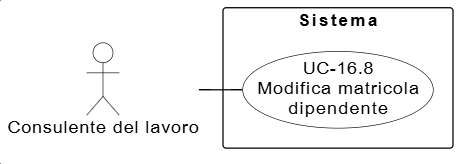
\includegraphics[width=0.65\textwidth]{diagrammi_use_case/uc_16.8.png}
    \caption{Diagramma del caso d'uso UC-16.8: Modifica matricola dipendente}
    \label{fig:uc-16.8}
\end{figure}
\begin{description}[style=multiline, leftmargin=4cm, font=\bfseries]
    \item[\glslink{attore}{Attore} Principale] \glslink{consulente-del-lavoro-cdl}{Consulente del lavoro}
    \item[Pre-condizioni] Il sistema è in modalità modifica del documento (UC-16) e il campo matricola è visibile nel pannello dati estratti.
    \item[Post-condizioni] Il sistema aggiorna la matricola del dipendente e la registra in attesa del salvataggio finale; eventuale link alla scheda dipendente viene aggiornato.
    \item[\glslink{scenario-principale}{Scenario Principale}]
    \begin{enumerate}[leftmargin=*, nosep]
        \item Il \glslink{consulente-del-lavoro-cdl}{Consulente del lavoro} seleziona il campo matricola.
        \item Il \glslink{consulente-del-lavoro-cdl}{Consulente del lavoro} inserisce o modifica la matricola.
        \item Il sistema verifica l'unicità o la corrispondenza con la scheda dipendente e segnala eventuali conflitti.
        \item Il sistema registra il valore aggiornato in attesa del salvataggio finale.
    \end{enumerate}
\end{description}

\paragraph{UC-16.6.E1: Errore - Formato email non valido}
\mbox{} \\

\begin{figure}[H]
    \centering
    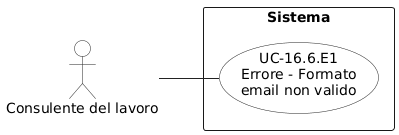
\includegraphics[width=0.65\textwidth]{diagrammi_use_case/uc_16.6.E1.png}
    \caption{Diagramma del caso d'uso UC-16.6.E1: Errore per formato email non valido}
    \label{fig:uc-16.6.e1}
\end{figure}
\begin{description}[style=multiline, leftmargin=4cm, font=\bfseries]
    \item[\glslink{attore}{Attore} Principale] \glslink{consulente-del-lavoro-cdl}{Consulente del lavoro}
    \item[Pre-condizioni] Il \glslink{consulente-del-lavoro-cdl}{Consulente del lavoro} sta modificando il campo email destinatario (UC-16.6) e ha inserito un indirizzo con formato non valido.
    \item[Post-condizioni] Il sistema segnala l'errore e non registra il valore finché non viene fornito un indirizzo e-mail con formato corretto.
    \item[\glslink{scenario-principale}{Scenario Principale}]
    \begin{enumerate}[leftmargin=*, nosep]
        \item Il sistema intercetta il formato e-mail non valido.
        \item Il sistema evidenzia il campo errato e richiede l'inserimento di un indirizzo e-mail corretto.
    \end{enumerate}
\end{description}

\paragraph{UC-16.7.E1: Errore - Codice fiscale non valido}
\mbox{} \\

\begin{figure}[H]
    \centering
    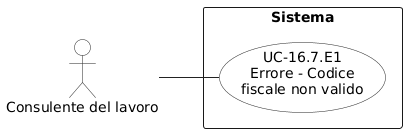
\includegraphics[width=0.65\textwidth]{diagrammi_use_case/uc_16.7.E1.png}
    \caption{Diagramma del caso d'uso UC-16.7.E1: Errore per codice fiscale non valido}
    \label{fig:uc-16.7.e1}
\end{figure}
\begin{description}[style=multiline, leftmargin=4cm, font=\bfseries]
    \item[\glslink{attore}{Attore} Principale] \glslink{consulente-del-lavoro-cdl}{Consulente del lavoro}
    \item[Pre-condizioni] Il \glslink{consulente-del-lavoro-cdl}{Consulente del lavoro} sta modificando il campo codice fiscale (UC-16.7) e il valore inserito non supera il controllo di validità formale (checksum).
    \item[Post-condizioni] Il sistema segnala l'incongruenza e non registra il valore finché non viene fornito un codice fiscale corretto.
    \item[\glslink{scenario-principale}{Scenario Principale}]
    \begin{enumerate}[leftmargin=*, nosep]
        \item Il sistema rileva che il codice fiscale inserito non supera il controllo di validità formale (checksum).
        \item Il sistema evidenzia il campo e segnala l'incongruenza, richiedendo la correzione del codice fiscale.
    \end{enumerate}
\end{description}

\subsubsection{UC-17: Generazione contenuto per l'invio}
\mbox{} \\

\begin{figure}[H]
    \centering
    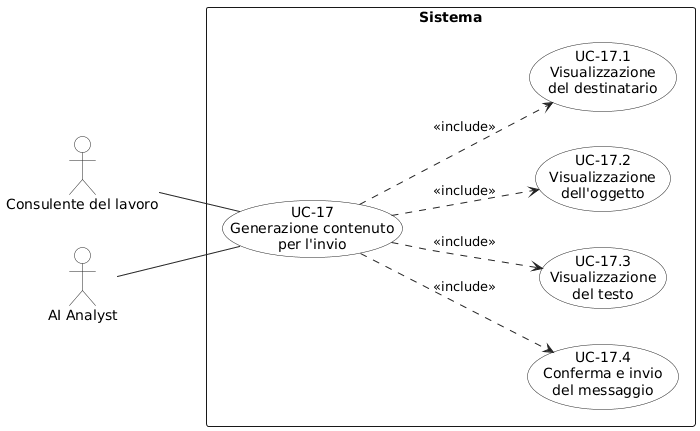
\includegraphics[width=1\textwidth]{diagrammi_use_case/uc_17.png}
    \caption{Diagramma del caso d'uso UC-17: Generazione contenuto per l'invio}
    \label{fig:uc-17}
\end{figure}
\begin{description}[style=multiline, leftmargin=4cm, font=\bfseries]
    \item[\glslink{attore}{Attore} Principale] \glslink{consulente-del-lavoro-cdl}{Consulente del lavoro}
    \item[\glslink{trigger}{Trigger}] Dopo la visualizzazione del singolo documento (UC-15), il \glslink{consulente-del-lavoro-cdl}{Consulente del lavoro} seleziona il comando di invio.
    \item[Pre-condizioni] Il \glslink{consulente-del-lavoro-cdl}{Consulente del lavoro} sta visualizzando il dettaglio di un documento nello storico (UC-15).
    \item[Post-condizioni] Il sistema invia il documento allegato al destinatario selezionato, utilizzando oggetto e testo confermati dal \glslink{consulente-del-lavoro-cdl}{Consulente del lavoro}.
    \item[\glslink{scenario-principale}{Scenario Principale}]
    \begin{enumerate}[leftmargin=*, nosep]
        \item Il \glslink{consulente-del-lavoro-cdl}{Consulente del lavoro} clicca il tasto "Invia" dalla vista di dettaglio del documento.
        \item Il sistema apre la sezione di generazione per l'invio e allega automaticamente il documento che era in visualizzazione.
        \item Il \glslink{consulente-del-lavoro-cdl}{Consulente del lavoro} visualizza il destinatario proposto dal sistema (\textbf{UC-17.1}).
        \item Il \glslink{consulente-del-lavoro-cdl}{Consulente del lavoro} visualizza l'oggetto proposto dal sistema (\textbf{UC-17.2}).
        \item Il \glslink{consulente-del-lavoro-cdl}{Consulente del lavoro} visualizza il testo proposto dal sistema (\textbf{UC-17.3}).
        \item Il \glslink{consulente-del-lavoro-cdl}{Consulente del lavoro} conferma l'invio e il sistema esegue la spedizione del messaggio (\textbf{UC-17.4}).
    \end{enumerate}
    \item[Relazioni]
    \begin{itemize}[leftmargin=*, nosep]
        \item \textbf{Inclusioni}: UC-17.1, UC-17.2, UC-17.3, UC-17.4.
    \end{itemize}
\end{description}

\paragraph{UC-17.1: Visualizzazione del destinatario}
\mbox{} \\

\begin{figure}[H]
    \centering
    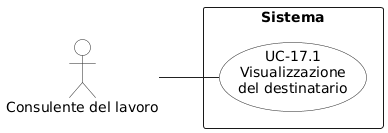
\includegraphics[width=0.65\textwidth]{diagrammi_use_case/uc_17.1.png}
    \caption{Diagramma del caso d'uso UC-17.1: Visualizzazione del destinatario}
    \label{fig:uc-17.1}
\end{figure}
\begin{description}[style=multiline, leftmargin=4cm, font=\bfseries]
    \item[\glslink{attore}{Attore} Principale] \glslink{consulente-del-lavoro-cdl}{Consulente del lavoro}
    \item[Pre-condizioni] Il sistema dispone del nome e cognome estratti dal documento selezionato.
    \item[Post-condizioni] Il \glslink{consulente-del-lavoro-cdl}{Consulente del lavoro} visualizza il destinatario proposto nel campo dedicato.
    \item[\glslink{scenario-principale}{Scenario Principale}]
    \begin{enumerate}[leftmargin=*, nosep]
        \item Il sistema propone il destinatario sulla base dei dati estratti dal documento.
        \item Il \glslink{consulente-del-lavoro-cdl}{Consulente del lavoro} visualizza il valore del campo destinatario.
    \end{enumerate}
\end{description}

\paragraph{UC-17.2: Visualizzazione dell'oggetto}
\mbox{} \\

\begin{figure}[H]
    \centering
    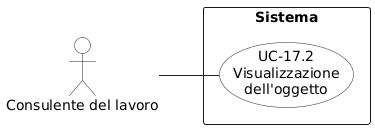
\includegraphics[width=0.65\textwidth]{diagrammi_use_case/uc_17.2.png}
    \caption{Diagramma del caso d'uso UC-17.2: Visualizzazione dell'oggetto}
    \label{fig:uc-17.2}
\end{figure}
\begin{description}[style=multiline, leftmargin=4cm, font=\bfseries]
    \item[\glslink{attore}{Attore} Principale] \glslink{consulente-del-lavoro-cdl}{Consulente del lavoro}
    \item[Pre-condizioni] Il sistema ha accesso \glslink{intelligenza-artificiale-ai}{ai} \glslink{metadati}{metadati} principali del documento selezionato.
    \item[Post-condizioni] Il \glslink{consulente-del-lavoro-cdl}{Consulente del lavoro} visualizza l'oggetto proposto nel campo dedicato.
    \item[\glslink{scenario-principale}{Scenario Principale}]
    \begin{enumerate}[leftmargin=*, nosep]
        \item Il sistema propone un oggetto coerente con il documento in invio.
        \item Il \glslink{consulente-del-lavoro-cdl}{Consulente del lavoro} visualizza il valore del campo oggetto.
    \end{enumerate}
\end{description}

\paragraph{UC-17.3: Visualizzazione del testo}
\mbox{} \\

\begin{figure}[H]
    \centering
    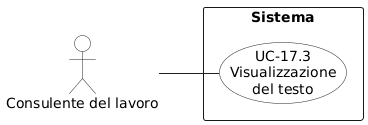
\includegraphics[width=0.65\textwidth]{diagrammi_use_case/uc_17.3.png}
    \caption{Diagramma del caso d'uso UC-17.3: Visualizzazione del testo}
    \label{fig:uc-17.3}
\end{figure}
\begin{description}[style=multiline, leftmargin=4cm, font=\bfseries]
    \item[\glslink{attore}{Attore} Principale] \glslink{consulente-del-lavoro-cdl}{Consulente del lavoro}
    \item[Pre-condizioni] Il sistema ha accesso \glslink{intelligenza-artificiale-ai}{ai} dati estratti dal documento selezionato.
    \item[Post-condizioni] Il \glslink{consulente-del-lavoro-cdl}{Consulente del lavoro} visualizza il testo proposto nel campo dedicato.
    \item[\glslink{scenario-principale}{Scenario Principale}]
    \begin{enumerate}[leftmargin=*, nosep]
        \item Il sistema propone un testo di accompagnamento del documento allegato.
        \item Il \glslink{consulente-del-lavoro-cdl}{Consulente del lavoro} visualizza il valore del campo testo.
    \end{enumerate}
\end{description}

\paragraph{UC-17.4: Conferma e invio del messaggio}
\mbox{} \\

\begin{figure}[H]
    \centering
    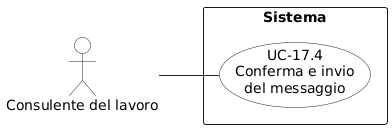
\includegraphics[width=0.65\textwidth]{diagrammi_use_case/uc_17.4.png}
    \caption{Diagramma del caso d'uso UC-17.4: Conferma e invio del messaggio}
    \label{fig:uc-17.4}
\end{figure}
\begin{description}[style=multiline, leftmargin=4cm, font=\bfseries]
    \item[\glslink{attore}{Attore} Principale] \glslink{consulente-del-lavoro-cdl}{Consulente del lavoro}
    \item[Pre-condizioni] Il \glslink{consulente-del-lavoro-cdl}{Consulente del lavoro} ha confermato destinatario, oggetto e testo nella schermata di invio.
    \item[Post-condizioni] Il sistema invia il messaggio con il documento allegato e notifica l'esito dell'operazione.
    \item[\glslink{scenario-principale}{Scenario Principale}]
    \begin{enumerate}[leftmargin=*, nosep]
        \item Il \glslink{consulente-del-lavoro-cdl}{Consulente del lavoro} seleziona l'invio definitivo del messaggio.
        \item Il sistema acquisisce i campi confermati e il documento allegato dalla schermata di invio.
        \item Il sistema invia il messaggio al destinatario indicato.
        \item Il sistema notifica al \glslink{consulente-del-lavoro-cdl}{Consulente del lavoro} l'esito dell'invio.
    \end{enumerate}
\end{description}

\subsubsection{UC-18: Modifica contenuto generato per l'invio}
\mbox{} \\

\begin{figure}[H]
    \centering
    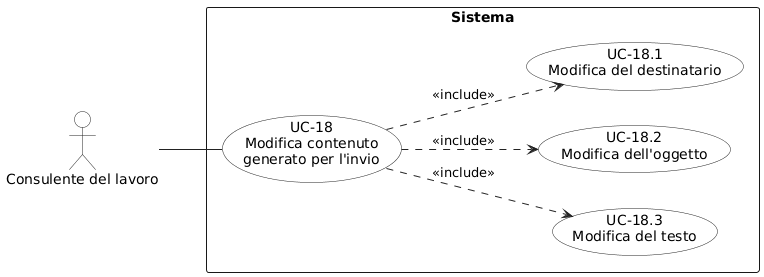
\includegraphics[width=1.1\textwidth]{diagrammi_use_case/uc_18.png}
    \caption{Diagramma del caso d'uso UC-18: Modifica contenuto generato per l'invio}
    \label{fig:uc-18}
\end{figure}
\begin{description}[style=multiline, leftmargin=4cm, font=\bfseries]
    \item[\glslink{attore}{Attore} Principale] \glslink{consulente-del-lavoro-cdl}{Consulente del lavoro}
    \item[\glslink{trigger}{Trigger}] Il \glslink{consulente-del-lavoro-cdl}{Consulente del lavoro} intende personalizzare la \glslink{bozza-draft}{bozza} di invio generata automaticamente (UC-17).
    \item[Pre-condizioni] Il sistema ha già predisposto la \glslink{bozza-draft}{bozza} di invio con destinatario, oggetto e testo.
    \item[Post-condizioni] Il sistema aggiorna i campi destinatario, oggetto e testo secondo le modifiche del \glslink{consulente-del-lavoro-cdl}{Consulente del lavoro}, rendendoli disponibili per l'invio in UC-17.
    \item[\glslink{scenario-principale}{Scenario Principale}]
    \begin{enumerate}[leftmargin=*, nosep]
        \item Il \glslink{consulente-del-lavoro-cdl}{Consulente del lavoro} modifica il destinatario proposto dal sistema (\textbf{UC-18.1}).
        \item Il \glslink{consulente-del-lavoro-cdl}{Consulente del lavoro} modifica l'oggetto proposto dal sistema (\textbf{UC-18.2}).
        \item Il \glslink{consulente-del-lavoro-cdl}{Consulente del lavoro} modifica il testo proposto dal sistema (\textbf{UC-18.3}).
        \item Il \glslink{consulente-del-lavoro-cdl}{Consulente del lavoro} conferma i campi aggiornati e ritorna al flusso di invio (UC-17).
    \end{enumerate}
    \item[Relazioni]
    \begin{itemize}[leftmargin=*, nosep]
        \item \textbf{Inclusioni}: UC-18.1, UC-18.2, UC-18.3.
    \end{itemize}
\end{description}

\paragraph{UC-18.1: Modifica del destinatario}
\mbox{} \\

\begin{figure}[H]
    \centering
    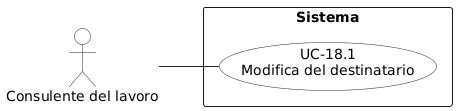
\includegraphics[width=0.7\textwidth]{diagrammi_use_case/uc_18.1.png}
    \caption{Diagramma del caso d'uso UC-18.1: Modifica del destinatario}
    \label{fig:uc-18.1}
\end{figure}
\begin{description}[style=multiline, leftmargin=4cm, font=\bfseries]
    \item[\glslink{attore}{Attore} Principale] \glslink{consulente-del-lavoro-cdl}{Consulente del lavoro}
    \item[Pre-condizioni] Il sistema mostra un destinatario precompilato nella \glslink{bozza-draft}{bozza} di invio.
    \item[Post-condizioni] Il campo destinatario contiene il valore aggiornato.
    \item[\glslink{scenario-principale}{Scenario Principale}]
    \begin{enumerate}[leftmargin=*, nosep]
        \item Il \glslink{consulente-del-lavoro-cdl}{Consulente del lavoro} sostituisce o integra il destinatario proposto.
        \item Il sistema aggiorna il campo destinatario nella \glslink{bozza-draft}{bozza}.
    \end{enumerate}
\end{description}

\paragraph{UC-18.2: Modifica dell'oggetto}
\mbox{} \\

\begin{figure}[H]
    \centering
    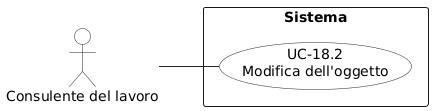
\includegraphics[width=0.7\textwidth]{diagrammi_use_case/uc_18.2.png}
    \caption{Diagramma del caso d'uso UC-18.2: Modifica dell'oggetto}
    \label{fig:uc-18.2}
\end{figure}
\begin{description}[style=multiline, leftmargin=4cm, font=\bfseries]
    \item[\glslink{attore}{Attore} Principale] \glslink{consulente-del-lavoro-cdl}{Consulente del lavoro}
    \item[Pre-condizioni] Il sistema mostra un oggetto precompilato nella \glslink{bozza-draft}{bozza} di invio.
    \item[Post-condizioni] Il campo oggetto contiene il valore aggiornato.
    \item[\glslink{scenario-principale}{Scenario Principale}]
    \begin{enumerate}[leftmargin=*, nosep]
        \item Il \glslink{consulente-del-lavoro-cdl}{Consulente del lavoro} modifica l'oggetto del messaggio.
        \item Il sistema aggiorna il campo oggetto nella \glslink{bozza-draft}{bozza}.
    \end{enumerate}
\end{description}

\paragraph{UC-18.3: Modifica del testo}
\mbox{} \\

\begin{figure}[H]
    \centering
    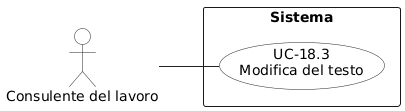
\includegraphics[width=0.7\textwidth]{diagrammi_use_case/uc_18.3.png}
    \caption{Diagramma del caso d'uso UC-18.3: Modifica del testo}
    \label{fig:uc-18.3}
\end{figure}
\begin{description}[style=multiline, leftmargin=4cm, font=\bfseries]
    \item[\glslink{attore}{Attore} Principale] \glslink{consulente-del-lavoro-cdl}{Consulente del lavoro}
    \item[Pre-condizioni] Il sistema mostra un testo precompilato nella \glslink{bozza-draft}{bozza} di invio.
    \item[Post-condizioni] Il campo testo contiene il valore aggiornato.
    \item[\glslink{scenario-principale}{Scenario Principale}]
    \begin{enumerate}[leftmargin=*, nosep]
        \item Il \glslink{consulente-del-lavoro-cdl}{Consulente del lavoro} modifica il testo del messaggio.
        \item Il sistema aggiorna il campo testo nella \glslink{bozza-draft}{bozza}.
    \end{enumerate}
\end{description}
\newpage
\subsubsection{UC-19: Dashboard metriche e monitoraggio AI Co-Pilot}
\mbox{} \\

\begin{figure}[H]
    \centering
    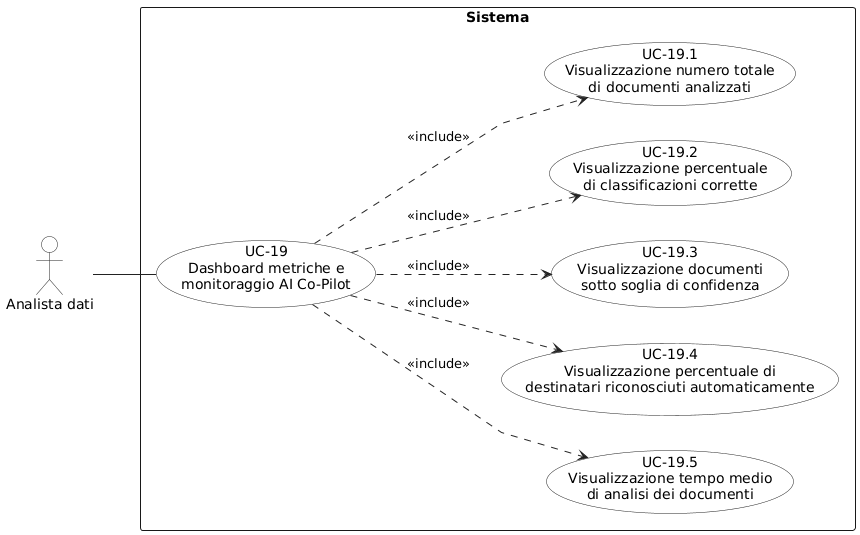
\includegraphics[width=1.1\textwidth]{diagrammi_use_case/uc_19.png}
    \caption{Diagramma del caso d'uso UC-19: Dashboard metriche e monitoraggio AI Co-Pilot}
    \label{fig:uc-19}
\end{figure}
\begin{description}[style=multiline, leftmargin=4cm, font=\bfseries]
    \item[\glslink{attore}{Attore} Principale] \glslink{analista-dati}{Analista dati}
    \item[\glslink{trigger}{Trigger}] L'\glslink{analista-dati}{Analista dati} intende consultare la \glslink{dashboard}{dashboard} delle metriche del modulo \glslink{intelligenza-artificiale-ai}{AI} Co-Pilot.
    \item[Pre-condizioni] L'\glslink{analista-dati}{Analista dati} è entrato nella sezione dedicata alle metriche del modulo \glslink{intelligenza-artificiale-ai}{AI} Co-Pilot.
    \item[Post-condizioni] L'\glslink{analista-dati}{Analista dati} ha visualizzato in \glslink{dashboard}{dashboard} i principali \glslink{kpi-key-performance-indicator}{KPI} del modulo \glslink{intelligenza-artificiale-ai}{AI} Co-Pilot.
    \item[\glslink{scenario-principale}{Scenario Principale}]
    \begin{enumerate}[leftmargin=*, nosep]
        \item Il sistema espone il numero totale di documenti analizzati; l'\glslink{analista-dati}{Analista dati} consulta il valore (\textbf{UC-19.1}).
        \item Il sistema espone la percentuale di classificazioni corrette; l'\glslink{analista-dati}{Analista dati} verifica il valore (\textbf{UC-19.2}).
        \item Il sistema espone la percentuale di documenti sotto \glslink{soglia-di-confidenza}{soglia di confidenza}; l'\glslink{analista-dati}{Analista dati} monitora il dato (\textbf{UC-19.3}).
        \item Il sistema espone la percentuale di destinatari riconosciuti automaticamente; l'\glslink{analista-dati}{Analista dati} verifica il valore (\textbf{UC-19.4}).
        \item Il sistema espone i tempi medi di analisi dell'\glslink{intelligenza-artificiale-ai}{intelligenza artificiale}; l'\glslink{analista-dati}{Analista dati} controlla il dato (\textbf{UC-19.5}).
    \end{enumerate}
    \item[Relazioni]
    \begin{itemize}[leftmargin=*, nosep]
        \item \textbf{Inclusioni}: UC-19.1, UC-19.2, UC-19.3, UC-19.4, UC-19.5.
    \end{itemize}
\end{description}

\paragraph{UC-19.1: Visualizzazione numero totale di documenti analizzati}
\mbox{} \\

\begin{figure}[H]
    \centering
    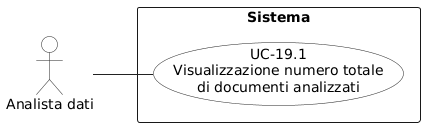
\includegraphics[width=0.7\textwidth]{diagrammi_use_case/uc_19.1.png}
    \caption{Diagramma del caso d'uso UC-19.1: Visualizzazione numero totale di documenti analizzati}
    \label{fig:uc-19.1}
\end{figure}
\begin{description}[style=multiline, leftmargin=4cm, font=\bfseries]
    \item[\glslink{attore}{Attore} Principale] \glslink{analista-dati}{Analista dati}
    \item[Pre-condizioni] L'\glslink{analista-dati}{Analista dati} si trova all'interno della \glslink{dashboard}{dashboard} delle metriche.
    \item[Post-condizioni] L'\glslink{analista-dati}{Analista dati} visualizza il numero totale dei documenti analizzati dal modulo \glslink{intelligenza-artificiale-ai}{AI} Co-Pilot.
    \item[\glslink{scenario-principale}{Scenario Principale}]
    \begin{enumerate}[leftmargin=*, nosep]
        \item Il sistema visualizza il numero totale complessivo di tutti i documenti processati dall'\glslink{intelligenza-artificiale-ai}{intelligenza artificiale}.
        \item L'\glslink{analista-dati}{Analista dati} osserva l'indicatore relativo \glslink{intelligenza-artificiale-ai}{ai} volumi di utilizzo.
    \end{enumerate}
\end{description}

\paragraph{UC-19.2: Visualizzazione percentuale di classificazioni corrette}
\mbox{} \\

\begin{figure}[H]
    \centering
    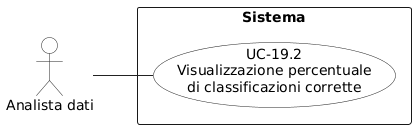
\includegraphics[width=0.7\textwidth]{diagrammi_use_case/uc_19.2.png}
    \caption{Diagramma del caso d'uso UC-19.2: Visualizzazione percentuale di classificazioni corrette}
    \label{fig:uc-19.2}
\end{figure}
\begin{description}[style=multiline, leftmargin=4cm, font=\bfseries]
    \item[\glslink{attore}{Attore} Principale] \glslink{analista-dati}{Analista dati}
    \item[Pre-condizioni] L'\glslink{analista-dati}{Analista dati} si trova all'interno della \glslink{dashboard}{dashboard} delle metriche.
    \item[Post-condizioni] L'\glslink{analista-dati}{Analista dati} visualizza la percentuale di classificazioni corrette effettuate automaticamente dall'\glslink{intelligenza-artificiale-ai}{AI}.
    \item[\glslink{scenario-principale}{Scenario Principale}]
    \begin{enumerate}[leftmargin=*, nosep]
        \item Il sistema visualizza la percentuale complessiva di documenti classificati correttamente dall'\glslink{intelligenza-artificiale-ai}{AI} sul totale analizzato, calcolata considerando solo i casi che non hanno richiesto alcun intervento manuale da parte degli operatori.
        \item L'\glslink{analista-dati}{Analista dati} osserva la metrica relativa all'accuratezza del sistema.
    \end{enumerate}
\end{description}

\paragraph{UC-19.3: Visualizzazione documenti sotto soglia di confidenza}
\mbox{} \\

\begin{figure}[H]
    \centering
    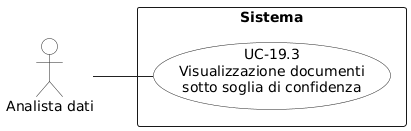
\includegraphics[width=0.7\textwidth]{diagrammi_use_case/uc_19.3.png}
    \caption{Diagramma del caso d'uso UC-19.3: Visualizzazione documenti sotto soglia di confidenza}
    \label{fig:uc-19.3}
\end{figure}
\begin{description}[style=multiline, leftmargin=4cm, font=\bfseries]
    \item[\glslink{attore}{Attore} Principale] \glslink{analista-dati}{Analista dati}
    \item[Pre-condizioni] L'\glslink{analista-dati}{Analista dati} si trova all'interno della \glslink{dashboard}{dashboard} delle metriche.
    \item[Post-condizioni] L'\glslink{analista-dati}{Analista dati} visualizza numero e percentuale dei documenti con \glslink{confidenza-confidence-score}{confidenza} inferiore alla soglia prevista.
    \item[\glslink{scenario-principale}{Scenario Principale}]
    \begin{enumerate}[leftmargin=*, nosep]
        \item Il sistema visualizza il numero totale e la relativa percentuale dei documenti per i quali l'\glslink{intelligenza-artificiale-ai}{AI} ha stimato una \glslink{confidenza-confidence-score}{confidenza} inferiore all'80\%, e che per questo motivo hanno richiesto una revisione umana.
        \item L'\glslink{analista-dati}{Analista dati} osserva le percentuali relative all'accuratezza del sistema.
    \end{enumerate}
\end{description}
\newpage
\paragraph{UC-19.4: Visualizzazione percentuale di destinatari riconosciuti automaticamente}
\mbox{} \\

\begin{figure}[H]
    \centering
    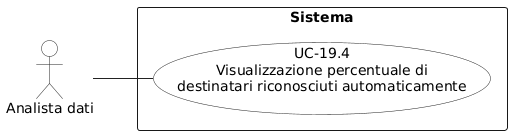
\includegraphics[width=0.85\textwidth]{diagrammi_use_case/uc_19.4.png}
    \caption{Diagramma del caso d'uso UC-19.4: Visualizzazione percentuale di destinatari riconosciuti automaticamente}
    \label{fig:uc-19.4}
\end{figure}
\begin{description}[style=multiline, leftmargin=4cm, font=\bfseries]
    \item[\glslink{attore}{Attore} Principale] \glslink{analista-dati}{Analista dati}
    \item[Pre-condizioni] L'\glslink{analista-dati}{Analista dati} si trova all'interno della \glslink{dashboard}{dashboard} delle metriche.
    \item[Post-condizioni] L'\glslink{analista-dati}{Analista dati} visualizza la percentuale di associazioni destinatario-anagrafica risolte automaticamente e correttamente dall'\glslink{intelligenza-artificiale-ai}{AI}.
    \item[\glslink{scenario-principale}{Scenario Principale}]
    \begin{enumerate}[leftmargin=*, nosep]
        \item Il sistema visualizza la percentuale complessiva di documenti in cui l'associazione tra il destinatario e la sua anagrafica è stata risolta in modo automatico e corretto dall'\glslink{intelligenza-artificiale-ai}{AI}.
        \item L'\glslink{analista-dati}{Analista dati} osserva il dato relativo allo smistamento dei file.
    \end{enumerate}
\end{description}

\paragraph{UC-19.5: Visualizzazione tempo medio di analisi dei documenti}
\mbox{} \\

\begin{figure}[H]
    \centering
    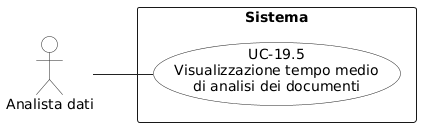
\includegraphics[width=0.7\textwidth]{diagrammi_use_case/uc_19.5.png}
    \caption{Diagramma del caso d'uso UC-19.5: Visualizzazione tempo medio di analisi dei documenti}
    \label{fig:uc-19.5}
\end{figure}
\begin{description}[style=multiline, leftmargin=4cm, font=\bfseries]
    \item[\glslink{attore}{Attore} Principale] \glslink{analista-dati}{Analista dati}
    \item[Pre-condizioni] L'\glslink{analista-dati}{Analista dati} si trova all'interno della \glslink{dashboard}{dashboard} delle metriche.
    \item[Post-condizioni] L'\glslink{analista-dati}{Analista dati} visualizza il tempo medio necessario all'\glslink{intelligenza-artificiale-ai}{AI} per completare l'analisi di un documento.
    \item[\glslink{scenario-principale}{Scenario Principale}]
    \begin{enumerate}[leftmargin=*, nosep]
        \item Il sistema visualizza il tempo medio impiegato dall'\glslink{intelligenza-artificiale-ai}{AI} per elaborare interamente un documento caricato e restituirne l'analisi completa all'utente.
        \item L'\glslink{analista-dati}{Analista dati} osserva l'indicatore delle prestazioni di sistema.
    \end{enumerate}
\end{description}





\newpage
\section{Requisiti}

Questa sezione raccoglie i requisiti individuati a partire dall'analisi dei casi d'uso descritti nelle sezioni precedenti. I requisiti sono organizzati nelle seguenti categorie:
\begin{itemize}
    \item \textbf{Requisiti funzionali} (RF): descrivono le funzionalità che il sistema deve offrire agli utenti;
    \item \textbf{Requisiti di qualità} (RQ): definiscono gli standard di processo e di prodotto che il gruppo deve rispettare;
    \item \textbf{Requisiti di vincolo} (RVC): specificano i limiti tecnologici entro cui il sistema deve essere sviluppato.
\end{itemize}

Ogni requisito è identificato da un codice univoco nella forma \textbf{\textit{categoria\_n}-\textit{priorità}}, dove il suffisso indica il grado di obbligatorietà:
\begin{itemize}
    \item \textbf{-OB} — Obbligatorio: il requisito deve essere soddisfatto senza eccezioni;
    \item \textbf{-OP} — Opzionale: il requisito è migliorativo e può essere valutato in fasi successive del progetto.
\end{itemize}

Ogni requisito è inoltre tracciato verso la fonte da cui è stato derivato (\glslink{caso-d-uso-uc}{caso d'uso}, \glslink{capitolato}{capitolato} o decisione interna).

\subsection{Requisiti funzionali}

I requisiti funzionali specificano le funzionalità che il sistema deve mettere a disposizione degli utenti, derivate dall'analisi dei casi d'uso.

\vspace{0.4cm}
{\small
\renewcommand{\arraystretch}{1.3}
\begin{longtable}{|p{2.5cm}|p{9.5cm}|p{3.5cm}|}
    \caption{Requisiti funzionali} \label{tab:rf} \\
    \hline
    \rowcolor{gray!20}
    \textbf{Codice} & \textbf{Descrizione} & \textbf{Fonte} \\
    \hline
    \endfirsthead
    \hline
    \rowcolor{gray!20}
    \textbf{Codice} & \textbf{Descrizione} & \textbf{Fonte} \\
    \hline
    \endhead
    \hline
    \endfoot
    \hline
    \endlastfoot

    \multicolumn{3}{|l|}{\cellcolor{gray!12}\textbf{\glslink{ai-assistant-generativo}{AI Assistant Generativo}}} \\
    \hline
    RF1-OB & Il sistema deve permettere al \glslink{redattore}{Redattore} di compilare il \glslink{prompt}{prompt} testuale descrittivo del contenuto da generare. & \hyperref[fig:uc-1.1]{UC-1.1} \\
    \hline
    RF2-OB & Il sistema deve permettere al \glslink{redattore}{Redattore} di selezionare il \glslink{tono-comunicativo}{tono comunicativo} della \glslink{bozza-draft}{bozza} da generare. & \hyperref[fig:uc-1.2]{UC-1.2} \\
    \hline
    RF3-OB & Il sistema deve permettere al \glslink{redattore}{Redattore} di selezionare lo \glslink{stile-editoriale}{stile editoriale} della \glslink{bozza-draft}{bozza} da generare. & \hyperref[fig:uc-1.3]{UC-1.3} \\
    \hline
    RF4-OP & Il sistema deve permettere al \glslink{redattore}{Redattore} di selezionare la lunghezza desiderata per la \glslink{bozza-draft}{bozza} da generare. & \hyperref[fig:uc-1.6]{UC-1.6} \\
    \hline
    RF5-OB & Il sistema deve permettere al \glslink{redattore}{Redattore} di salvare la configurazione corrente del \glslink{prompt}{prompt} nella libreria personale, assegnandole un nome identificativo. & \hyperref[fig:uc-1.4]{UC-1.4} \\
    \hline
    RF6-OB & Il sistema deve permettere al \glslink{redattore}{Redattore} di svuotare i campi di configurazione, ripristinando i valori predefiniti. & \hyperref[fig:uc-1.5]{UC-1.5} \\
    \hline
    RF7-OB & Il sistema deve avviare la generazione del contenuto tramite il modulo \glslink{ai-post-generator}{AI Post Generator} a partire dal \glslink{prompt}{prompt} e dai parametri configurati. & \hyperref[fig:uc-1]{UC-1} \\
    \hline
    RF8-OB & Il sistema deve notificare il \glslink{redattore}{Redattore} qualora il campo \glslink{prompt}{prompt} sia assente o insufficiente prima dell'avvio della generazione. & \hyperref[fig:uc-1.e1]{UC-1.E1} \\
    \hline
    RF9-OB & Il sistema deve notificare il \glslink{redattore}{Redattore} in caso di errore interno o \glslink{timeout}{timeout} durante la generazione iniziale del contenuto tramite \glslink{intelligenza-artificiale-ai}{AI}. & \hyperref[fig:uc-1.e2]{UC-1.E2} \\
    \hline
    RF10-OB & Il sistema deve notificare il \glslink{redattore}{Redattore} in caso di errore interno o \glslink{timeout}{timeout} durante la rigenerazione del contenuto tramite \glslink{intelligenza-artificiale-ai}{AI}. & \hyperref[fig:uc-2.7.e1]{UC-2.7.E1} \\
    \hline
    RF11-OB & Il sistema deve visualizzare un'anteprima della \glslink{bozza-draft}{bozza} generata. & \hyperref[fig:uc-2]{UC-2} \\
    \hline
    RF12-OB & Il sistema deve visualizzare il titolo della \glslink{bozza-draft}{bozza} generata nell'anteprima. & \hyperref[fig:uc-2.1]{UC-2.1} \\
    \hline
    RF13-OB & Il sistema deve visualizzare il testo della \glslink{bozza-draft}{bozza} generata nell'anteprima. & \hyperref[fig:uc-2.2]{UC-2.2} \\
    \hline
    RF14-OB & Il sistema deve visualizzare l'immagine di copertina della \glslink{bozza-draft}{bozza} generata nell'anteprima. & \hyperref[fig:uc-2.3]{UC-2.3} \\
    \hline
    RF15-OB & Il sistema deve permettere al \glslink{redattore}{Redattore} di modificare manualmente il titolo della \glslink{bozza-draft}{bozza}. & \hyperref[fig:uc-2.4]{UC-2.4} \\
    \hline
    RF16-OB & Il sistema deve permettere al \glslink{redattore}{Redattore} di modificare manualmente il testo della \glslink{bozza-draft}{bozza}. & \hyperref[fig:uc-2.5]{UC-2.5} \\
    \hline
    RF17-OB & Il sistema deve permettere al \glslink{redattore}{Redattore} di sostituire l'immagine di copertina della \glslink{bozza-draft}{bozza} con un file caricato localmente. & \hyperref[fig:uc-2.6]{UC-2.6} \\
    \hline
    RF18-OB & Il sistema deve notificare il \glslink{redattore}{Redattore} in caso di formato file non valido durante la sostituzione dell'immagine di copertina. & \hyperref[fig:uc-2.6.e1]{UC-2.6.E1} \\
    \hline
    RF19-OB & Il sistema deve permettere al \glslink{redattore}{Redattore} di richiedere la rigenerazione della \glslink{bozza-draft}{bozza} mantenendo i parametri di configurazione. & \hyperref[fig:uc-2.7]{UC-2.7} \\
    \hline
    RF20-OB & Il sistema deve permettere al \glslink{redattore}{Redattore} di eliminare la \glslink{bozza-draft}{bozza} generata corrente. & \hyperref[fig:uc-2.8]{UC-2.8} \\
    \hline
    RF21-OP & Il sistema deve permettere al \glslink{redattore}{Redattore} di annullare le modifiche manuali apportate alla \glslink{bozza-draft}{bozza}, ripristinando il contenuto originariamente generato. & \hyperref[fig:uc-2.9]{UC-2.9} \\
    \hline
    RF22-OB & Il sistema deve notificare il \glslink{redattore}{Redattore} qualora il contenuto della \glslink{bozza-draft}{bozza} risulti vuoto a seguito di modifiche. & \hyperref[fig:uc-2.e1]{UC-2.E1} \\
    \hline
    RF23-OB & Il sistema deve permettere al \glslink{redattore}{Redattore} di approvare e finalizzare il documento generato. & \hyperref[fig:uc-3]{UC-3} \\
    \hline
    RF24-OB & Il sistema deve visualizzare le opzioni disponibili per la finalizzazione del documento (salvataggio in \glslink{bozza-draft}{bozza}, esportazione, inoltro). & \hyperref[fig:uc-3.1]{UC-3.1} \\
    \hline
    RF25-OB & Il sistema deve permettere il salvataggio del documento come \glslink{bozza-draft}{bozza} nello storico. & \hyperref[fig:uc-3.2]{UC-3.2} \\
    \hline
    RF26-OB & Il sistema deve permettere l'esportazione del documento finalizzato in formato PDF. & \hyperref[fig:uc-3.3]{UC-3.3} \\
    \hline
    RF27-OB & Il sistema deve permettere al \glslink{redattore}{Redattore} di inoltrare il documento finalizzato tramite posta elettronica. & \hyperref[fig:uc-3.4]{UC-3.4} \\
    \hline
    RF28-OP & Il sistema deve permettere al \glslink{redattore}{Redattore} di visualizzare un'anteprima del documento prima dell'esportazione definitiva. & \hyperref[fig:uc-3.5]{UC-3.5} \\
    \hline
    RF29-OB & Il sistema deve notificare il \glslink{redattore}{Redattore} in caso di indirizzo e-mail non valido durante l'inoltro. & \hyperref[fig:uc-3.4.e1]{UC-3.4.E1} \\
    \hline
    RF30-OB & Il sistema deve fornire al \glslink{redattore}{Redattore} una libreria personale dei \glslink{prompt}{prompt} con il relativo storico delle generazioni passate. & \hyperref[fig:uc-4]{UC-4} \\
    \hline
    RF31-OB & Il sistema deve permettere al \glslink{redattore}{Redattore} di visualizzare l'elenco delle generazioni passate e i \glslink{prompt}{prompt} salvati nella libreria personale. & \hyperref[fig:uc-4.1]{UC-4.1} \\
    \hline
    RF32-OB & Il sistema deve permettere la ricerca e il filtraggio dello storico dei \glslink{prompt}{prompt} e delle generazioni passate. & \hyperref[fig:uc-4.2]{UC-4.2} \\
    \hline
    RF33-OB & Il sistema deve avvisare l'utente quando la ricerca nello storico non produce risultati. & \hyperref[fig:uc-4.2.e1]{UC-4.2.E1} \\
    \hline
    RF34-OB & Il sistema deve permettere il caricamento e il riutilizzo di una configurazione \glslink{prompt}{prompt} dalla libreria personale. & \hyperref[fig:uc-4.3]{UC-4.3} \\
    \hline
    RF35-OB & Il sistema deve permettere al \glslink{redattore}{Redattore} di contrassegnare o rimuovere una generazione come preferita nella libreria personale. & \hyperref[fig:uc-4.4]{UC-4.4} \\
    \hline
    RF36-OP & Il sistema deve permettere l'eliminazione di elementi dallo storico e dalla libreria dei \glslink{prompt}{prompt}. & \hyperref[fig:uc-4.5]{UC-4.5} \\
    \hline
    RF37-OB & Il sistema deve fornire un modulo di valutazione qualitativa delle bozze generate. & \hyperref[fig:uc-5]{UC-5} \\
    \hline
    RF38-OB & Il sistema deve permettere al \glslink{redattore}{Redattore} di accedere al modulo di valutazione qualitativa della \glslink{bozza-draft}{bozza} generata. & \hyperref[fig:uc-5.1]{UC-5.1} \\
    \hline
    RF39-OB & Il sistema deve permettere al \glslink{redattore}{Redattore} di assegnare un \glslink{rating}{rating} numerico alla \glslink{bozza-draft}{bozza} generata. & \hyperref[fig:uc-5.2]{UC-5.2} \\
    \hline
    RF40-OB & Il sistema deve permettere al \glslink{redattore}{Redattore} di inserire un commento testuale opzionale nell'ambito della valutazione della \glslink{bozza-draft}{bozza}. & \hyperref[fig:uc-5.3]{UC-5.3} \\
    \hline
    RF41-OB & Il sistema deve permettere al \glslink{redattore}{Redattore} di inviare la valutazione al sistema. & \hyperref[fig:uc-5.4]{UC-5.4} \\
    \hline
    RF42-OB & Il sistema deve notificare il \glslink{redattore}{Redattore} qualora tenti di inviare la valutazione senza aver assegnato un \glslink{rating}{rating}. & \hyperref[fig:uc-5.4.e1]{UC-5.4.E1} \\
    \hline
    RF43-OB & Il sistema deve notificare il \glslink{redattore}{Redattore} qualora il commento testuale superi il limite di caratteri consentito. & \hyperref[fig:uc-5.3.e1]{UC-5.3.E1} \\
    \hline
    RF44-OB & Il sistema deve fornire all'\glslink{analista-dati}{Analista dati} una \glslink{dashboard}{dashboard} dedicata con metriche di utilizzo del modulo \glslink{ai-assistant-generativo}{AI Assistant Generativo}. & \hyperref[fig:uc-6]{UC-6} \\
    \hline
    RF45-OB & Il sistema deve visualizzare nella \glslink{dashboard}{dashboard} una panoramica dell'attività complessiva del modulo \glslink{intelligenza-artificiale-ai}{AI} Assistant. & \hyperref[fig:uc-6.1]{UC-6.1} \\
    \hline
    RF46-OB & Il sistema deve visualizzare nella \glslink{dashboard}{dashboard} le statistiche di utilizzo del modulo \glslink{intelligenza-artificiale-ai}{AI} Assistant. & \hyperref[fig:uc-6.2]{UC-6.2} \\
    \hline
    RF47-OB & Il sistema deve visualizzare nella \glslink{dashboard}{dashboard} il \glslink{rating}{rating} medio delle bozze generate. & \hyperref[fig:uc-6.3]{UC-6.3} \\
    \hline
    RF48-OB & Il sistema deve permettere all'\glslink{analista-dati}{Analista dati} di consultare i feedback testuali ricevuti dagli utenti. & \hyperref[fig:uc-6.4]{UC-6.4} \\
    \hline
    RF49-OB & Il sistema deve permettere all'\glslink{analista-dati}{Analista dati} di applicare filtri dinamici \glslink{intelligenza-artificiale-ai}{ai} dati visualizzati nella \glslink{dashboard}{dashboard} analitica (es. intervallo di date, tono, stile). & \hyperref[fig:uc-6.5]{UC-6.5} \\
    \hline
    RF50-OB & Il sistema deve permettere all'\glslink{analista-dati}{Analista dati} di esportare un report riepilogativo dei dati analitici in formato scaricabile. & \hyperref[fig:uc-6.6]{UC-6.6} \\
    \hline
    RF51-OB & Il sistema deve notificare l'\glslink{analista-dati}{Analista dati} qualora i dati non siano disponibili per l'esportazione del report. & \hyperref[fig:uc-6.6.e1]{UC-6.6.E1} \\
    \hline

    \multicolumn{3}{|l|}{\cellcolor{gray!12}\textbf{\glslink{ai-co-pilot-per-consulenti-del-lavoro-cdl}{AI Co-Pilot per Consulenti del Lavoro}}} \\
    \hline
    RF52-OB & Il sistema deve permettere al \glslink{consulente-del-lavoro-cdl}{Consulente del lavoro} di caricare singoli documenti o lotti nel \glslink{repository}{repository} dedicato. & \hyperref[fig:uc-7]{UC-7} \\
    \hline
    RF53-OB & Il sistema deve rilevare i documenti duplicati durante l'upload e notificare il \glslink{consulente-del-lavoro-cdl}{Consulente del lavoro}, richiedendone conferma prima del caricamento. & \hyperref[fig:uc-7.e1]{UC-7.E1} \\
    \hline
    RF54-OB & Il sistema deve rilevare i formati file non supportati durante l'upload e notificare il \glslink{consulente-del-lavoro-cdl}{Consulente del lavoro}. & \hyperref[fig:uc-7.e2]{UC-7.E2} \\
    \hline
    RF55-OB & Il sistema deve classificare automaticamente i documenti caricati e popolare i \glslink{metadati}{metadati} associati tramite il modulo \glslink{ai-analyst}{AI Analyst}. & \hyperref[fig:uc-8]{UC-8} \\
    \hline
    RF56-OB & Il sistema deve permettere al \glslink{consulente-del-lavoro-cdl}{Consulente del lavoro} di visualizzare lo storico dei documenti analizzati. & \hyperref[fig:uc-9]{UC-9} \\
    \hline
    RF57-OB & Il sistema deve notificare l'utente quando nessun documento corrisponde \glslink{intelligenza-artificiale-ai}{ai} criteri di visualizzazione dello storico. & \hyperref[fig:uc-9.e1]{UC-9.E1} \\
    \hline
    RF58-OB & Il sistema deve permettere il filtraggio dello storico documenti tramite criteri multipli. & \hyperref[fig:uc-10]{UC-10} \\
    \hline
    RF59-OB & Il sistema deve permettere il filtraggio dello storico documenti tramite barra di ricerca testuale. & \hyperref[fig:uc-11]{UC-11} \\
    \hline
    RF60-OB & Il sistema deve permettere il filtraggio dello storico documenti per stato di invio. & \hyperref[fig:uc-12]{UC-12} \\
    \hline
    RF61-OB & Il sistema deve permettere il filtraggio dello storico documenti per livello di \glslink{confidenza-confidence-score}{confidenza} dell'analisi \glslink{intelligenza-artificiale-ai}{AI}. & \hyperref[fig:uc-13]{UC-13} \\
    \hline
    RF62-OB & Il sistema deve permettere il filtraggio dello storico documenti per mese e anno. & \hyperref[fig:uc-14]{UC-14} \\
    \hline
    RF63-OB & Il sistema deve permettere al \glslink{consulente-del-lavoro-cdl}{Consulente del lavoro} di visualizzare i dettagli di un singolo documento dallo storico. & \hyperref[fig:uc-15]{UC-15} \\
    \hline
    RF64-OB & Il sistema deve permettere la visualizzazione del documento originale nella versione splittata. & \hyperref[fig:uc-15.1]{UC-15.1} \\
    \hline
    RF65-OB & Il sistema deve permettere la visualizzazione del documento originale non splittato. & \hyperref[fig:uc-15.2]{UC-15.2} \\
    \hline
    RF66-OB & Il sistema deve visualizzare il nome e cognome del destinatario associato al documento. & \hyperref[fig:uc-15.3]{UC-15.3} \\
    \hline
    RF67-OB & Il sistema deve visualizzare l'azienda associata al documento. & \hyperref[fig:uc-15.4]{UC-15.4} \\
    \hline
    RF68-OB & Il sistema deve visualizzare il nome del file del documento. & \hyperref[fig:uc-15.5]{UC-15.5} \\
    \hline
    RF69-OB & Il sistema deve visualizzare la data del documento. & \hyperref[fig:uc-15.6]{UC-15.6} \\
    \hline
    RF70-OB & Il sistema deve visualizzare il numero di pagine del documento. & \hyperref[fig:uc-15.7]{UC-15.7} \\
    \hline
    RF71-OB & Il sistema deve visualizzare la tipologia del documento. & \hyperref[fig:uc-15.8]{UC-15.8} \\
    \hline
    RF72-OB & Il sistema deve visualizzare la breve descrizione del documento. & \hyperref[fig:uc-15.9]{UC-15.9} \\
    \hline
    RF73-OB & Il sistema deve visualizzare il livello di \glslink{confidenza-confidence-score}{confidenza} in percentuale del documento. & \hyperref[fig:uc-15.10]{UC-15.10} \\
    \hline
    RF74-OB & Il sistema deve visualizzare lo stato di invio del documento. & \hyperref[fig:uc-15.11]{UC-15.11} \\
    \hline
    RF75-OP & Il sistema deve visualizzare l'e-mail del destinatario del documento. & \hyperref[fig:uc-15.12]{UC-15.12} \\
    \hline
    RF76-OP & Il sistema deve visualizzare il codice fiscale del destinatario. & \hyperref[fig:uc-15.13]{UC-15.13} \\
    \hline
    RF77-OP & Il sistema deve visualizzare la matricola del dipendente. & \hyperref[fig:uc-15.14]{UC-15.14} \\
    \hline
    RF78-OP & Il sistema deve visualizzare la data e ora di caricamento del documento. & \hyperref[fig:uc-15.15]{UC-15.15} \\
    \hline
    RF79-OB & Il sistema deve gestire il caso in cui il nome e cognome del destinatario non siano disponibili, visualizzando un opportuno indicatore. & \hyperref[fig:uc-15.3.e1]{UC-15.3.E1} \\
    \hline
    RF80-OB & Il sistema deve gestire il caso in cui l'azienda non sia disponibile, visualizzando un opportuno indicatore. & \hyperref[fig:uc-15.4.e1]{UC-15.4.E1} \\
    \hline
    RF81-OB & Il sistema deve gestire il caso in cui la data del documento non sia disponibile, visualizzando un opportuno indicatore. & \hyperref[fig:uc-15.6.e1]{UC-15.6.E1} \\
    \hline
    RF82-OB & Il sistema deve gestire il caso in cui la tipologia del documento non sia disponibile, visualizzando un opportuno indicatore. & \hyperref[fig:uc-15.8.e1]{UC-15.8.E1} \\
    \hline
    RF83-OB & Il sistema deve gestire il caso in cui la breve descrizione non sia disponibile, visualizzando un opportuno indicatore. & \hyperref[fig:uc-15.9.e1]{UC-15.9.E1} \\
    \hline
    RF84-OB & Il sistema deve gestire il caso in cui il livello di \glslink{confidenza-confidence-score}{confidenza} non sia disponibile, visualizzando un opportuno indicatore. & \hyperref[fig:uc-15.10.e1]{UC-15.10.E1} \\
    \hline
    RF85-OB & Il sistema deve permettere al \glslink{consulente-del-lavoro-cdl}{Consulente del lavoro} di modificare i \glslink{metadati}{metadati} di un documento presente nello storico. & \hyperref[fig:uc-16]{UC-16} \\
    \hline
    RF86-OB & Il sistema deve permettere la modifica del nome e cognome del destinatario associato al documento. & \hyperref[fig:uc-16.1]{UC-16.1} \\
    \hline
    RF87-OB & Il sistema deve permettere la modifica dell'azienda associata al documento. & \hyperref[fig:uc-16.2]{UC-16.2} \\
    \hline
    RF88-OB & Il sistema deve permettere la modifica della data del documento. & \hyperref[fig:uc-16.3]{UC-16.3} \\
    \hline
    RF89-OB & Il sistema deve permettere la modifica della tipologia del documento. & \hyperref[fig:uc-16.4]{UC-16.4} \\
    \hline
    RF90-OB & Il sistema deve permettere la modifica della breve descrizione del documento. & \hyperref[fig:uc-16.5]{UC-16.5} \\
    \hline
    RF91-OP & Il sistema deve permettere la modifica dell'indirizzo e-mail del destinatario. & \hyperref[fig:uc-16.6]{UC-16.6} \\
    \hline
    RF92-OP & Il sistema deve permettere la modifica del codice fiscale del destinatario. & \hyperref[fig:uc-16.7]{UC-16.7} \\
    \hline
    RF93-OP & Il sistema deve permettere la modifica della matricola del dipendente. & \hyperref[fig:uc-16.8]{UC-16.8} \\
    \hline
    RF94-OP & Il sistema deve notificare il \glslink{consulente-del-lavoro-cdl}{Consulente del lavoro} in caso di formato e-mail non valido durante la modifica. & \hyperref[fig:uc-16.6.e1]{UC-16.6.E1} \\
    \hline
    RF95-OP & Il sistema deve notificare il \glslink{consulente-del-lavoro-cdl}{Consulente del lavoro} in caso di codice fiscale non valido durante la modifica. & \hyperref[fig:uc-16.7.e1]{UC-16.7.E1} \\
    \hline
    RF96-OB & Il sistema deve generare automaticamente il contenuto del messaggio di invio per il documento da spedire. & \hyperref[fig:uc-17]{UC-17} \\
    \hline
    RF97-OB & Il sistema deve visualizzare il destinatario del messaggio di invio generato automaticamente. & \hyperref[fig:uc-17.1]{UC-17.1} \\
    \hline
    RF98-OB & Il sistema deve visualizzare l'oggetto del messaggio di invio generato automaticamente. & \hyperref[fig:uc-17.2]{UC-17.2} \\
    \hline
    RF99-OB & Il sistema deve visualizzare il testo del messaggio di invio generato automaticamente. & \hyperref[fig:uc-17.3]{UC-17.3} \\
    \hline
    RF100-OB & Il sistema deve permettere la conferma e l'effettivo invio del messaggio al destinatario. & \hyperref[fig:uc-17.4]{UC-17.4} \\
    \hline
    RF101-OB & Il sistema deve permettere al \glslink{consulente-del-lavoro-cdl}{Consulente del lavoro} di modificare il contenuto del messaggio di invio generato prima della spedizione. & \hyperref[fig:uc-18]{UC-18} \\
    \hline
    RF102-OB & Il sistema deve permettere la modifica del destinatario del messaggio di invio. & \hyperref[fig:uc-18.1]{UC-18.1} \\
    \hline
    RF103-OB & Il sistema deve permettere la modifica dell'oggetto del messaggio di invio. & \hyperref[fig:uc-18.2]{UC-18.2} \\
    \hline
    RF104-OB & Il sistema deve permettere la modifica del testo del messaggio di invio. & \hyperref[fig:uc-18.3]{UC-18.3} \\
    \hline
    RF105-OB & Il sistema deve fornire all'\glslink{analista-dati}{Analista dati} una \glslink{dashboard}{dashboard} dedicata con metriche di monitoraggio del modulo \glslink{intelligenza-artificiale-ai}{AI} Co-Pilot. & \hyperref[fig:uc-19]{UC-19} \\
    \hline
    RF106-OB & Il sistema deve visualizzare nella \glslink{dashboard}{dashboard} del Co-Pilot il numero totale di documenti analizzati. & \hyperref[fig:uc-19.1]{UC-19.1} \\
    \hline
    RF107-OB & Il sistema deve visualizzare nella \glslink{dashboard}{dashboard} del Co-Pilot la percentuale di classificazioni corrette. & \hyperref[fig:uc-19.2]{UC-19.2} \\
    \hline
    RF108-OB & Il sistema deve visualizzare nella \glslink{dashboard}{dashboard} del Co-Pilot i documenti sotto \glslink{soglia-di-confidenza}{soglia di confidenza}. & \hyperref[fig:uc-19.3]{UC-19.3} \\
    \hline
    RF109-OB & Il sistema deve visualizzare nella \glslink{dashboard}{dashboard} del Co-Pilot la percentuale di destinatari riconosciuti automaticamente. & \hyperref[fig:uc-19.4]{UC-19.4} \\
    \hline
    RF110-OB & Il sistema deve visualizzare nella \glslink{dashboard}{dashboard} del Co-Pilot il tempo medio di analisi dei documenti. & \hyperref[fig:uc-19.5]{UC-19.5} \\
    \hline

\end{longtable}
}
\newpage
\subsection{Requisiti di qualità}

I requisiti di qualità definiscono gli standard di processo e di prodotto che il gruppo deve rispettare durante lo sviluppo. Derivano principalmente dal \href{https://www.math.unipd.it/~tullio/IS-1/2025/Progetto/C5.pdf}{Capitolato C5} e dalle norme interne adottate dal gruppo.

\vspace{0.4cm}
{\small
\renewcommand{\arraystretch}{1.3}
\begin{longtable}{|p{2.5cm}|p{9.5cm}|p{3.5cm}|}
    \caption{Requisiti di qualità} \label{tab:rq} \\
    \hline
    \rowcolor{gray!20}
    \textbf{Codice} & \textbf{Descrizione} & \textbf{Fonte} \\
    \hline
    \endfirsthead
    \hline
    \rowcolor{gray!20}
    \textbf{Codice} & \textbf{Descrizione} & \textbf{Fonte} \\
    \hline
    \endhead
    \hline
    \endfoot
    \hline
    \endlastfoot

    RQ1-OB & Redazione dell'\glslink{analisi-dei-requisiti-adr}{Analisi dei Requisiti} comprensiva di casi d'uso modellati tramite UML. & \href{https://www.math.unipd.it/~tullio/IS-1/2025/Progetto/C5.pdf}{Capitolato} \\
    \hline
    RQ2-OB & Le pratiche di sviluppo devono essere conformi alle \glslink{norme-di-progetto}{Norme di Progetto} adottate dal gruppo. & Interna \\
    \hline
    RQ3-OB & Il prodotto deve superare tutti i test automatizzati con una copertura del codice (statement coverage) non inferiore all'80\%. & Interna \\
    \hline
    RQ4-OB & La documentazione del codice sorgente deve rispettare le convenzioni definite nelle \glslink{norme-di-progetto}{Norme di Progetto}. & \href{https://www.math.unipd.it/~tullio/IS-1/2025/Progetto/C5.pdf}{Capitolato}, Interna \\
    \hline
    RQ5-OB & Il sorgente deve essere gestito tramite un sistema di versionamento, con istruzioni di setup incluse nel \glslink{repository}{repository}. & \href{https://www.math.unipd.it/~tullio/IS-1/2025/Progetto/C5.pdf}{Capitolato} \\
    \hline
    RQ6-OB & Produzione di un manuale utente per il prodotto sviluppato. & \href{https://www.math.unipd.it/~tullio/IS-1/2025/Progetto/C5.pdf}{Capitolato} \\
    \hline
    RQ7-OB & Il modulo \glslink{intelligenza-artificiale-ai}{AI} Co-Pilot deve raggiungere una \glslink{confidenza-confidence-score}{confidenza} media \glslink{ocr-riconoscimento-ottico-dei-caratteri}{OCR} $\geq$ 90\% e un'accuratezza di mapping del codice fiscale $\geq$ 99\%; i documenti con \glslink{confidenza-confidence-score}{confidenza} inferiore alla soglia devono essere indirizzati alla revisione \glslink{human-in-the-loop}{human-in-the-loop}. & \href{https://www.math.unipd.it/~tullio/IS-1/2025/Progetto/C5.pdf}{Capitolato} \\
    \hline
    RQ8-OB & La qualità percepita dei contenuti generati dal modulo \glslink{intelligenza-artificiale-ai}{AI} Assistant deve risultare $\geq$ 4/5 nel sistema di \glslink{rating}{rating} utenti integrato. & \href{https://www.math.unipd.it/~tullio/IS-1/2025/Progetto/C5.pdf}{Capitolato} \\
    \hline
    RQ9-OB & L'interfaccia utente deve rimanere fluida e reattiva in ogni momento, anche durante l'elaborazione di operazioni in background. & \href{https://www.math.unipd.it/~tullio/IS-1/2025/Progetto/C5.pdf}{Capitolato} \\
    \hline
    RQ10-OB & Le operazioni computazionalmente onerose (classificazione \glslink{intelligenza-artificiale-ai}{AI}, generazione di contenuti, split documentale) devono essere eseguite in modo asincrono, senza bloccare l'interfaccia utente. & \href{https://www.math.unipd.it/~tullio/IS-1/2025/Progetto/C5.pdf}{Capitolato} \\
    \hline

\end{longtable}
}
\newpage
\subsection{Requisiti di vincolo}

I requisiti di vincolo definiscono i limiti tecnologici entro cui il sistema deve essere sviluppato, derivanti dalle scelte architetturali concordate con il \glslink{committente-proponente}{proponente} Eggon S.r.l.

\vspace{0.4cm}
{\small
\renewcommand{\arraystretch}{1.3}
\begin{longtable}{|p{2.5cm}|p{9.5cm}|p{3.5cm}|}
    \caption{Requisiti di vincolo} \label{tab:rvc} \\
    \hline
    \rowcolor{gray!20}
    \textbf{Codice} & \textbf{Descrizione} & \textbf{Fonte} \\
    \hline
    \endfirsthead
    \hline
    \rowcolor{gray!20}
    \textbf{Codice} & \textbf{Descrizione} & \textbf{Fonte} \\
    \hline
    \endhead
    \hline
    \endfoot
    \hline
    \endlastfoot

    \multicolumn{3}{|l|}{\cellcolor{gray!12}\textbf{Controllo versione e qualità del codice}} \\
    \hline
    RVC1-OB & Il codice sorgente deve essere versionato tramite \glslink{git}{Git} su un \glslink{repository}{repository} condiviso. & \glslink{committente-proponente}{Proponente} \\
    \hline
    RVC2-OB & Il codice sorgente deve rispettare le regole di formattazione definite da \glslink{laravel}{Laravel} Pint. & Interna \\
    \hline
    RVC3-OB & La suite di test automatizzati deve essere scritta con il framework \glslink{pest}{Pest}. & Interna \\
    \hline

    \multicolumn{3}{|l|}{\cellcolor{gray!12}\textbf{Backend}} \\
    \hline
    RVC4-OB & Il backend deve essere sviluppato con il framework \glslink{laravel}{Laravel} 12 su PHP 8.4. & Interna \\
    \hline
    RVC5-OB & Il database relazionale del sistema deve essere \glslink{postgresql}{PostgreSQL}. & Interna \\
    \hline
    RVC6-OB & Le code asincrone e la gestione dei job in background devono utilizzare \glslink{redis}{Redis}. & Interna \\
    \hline

    \multicolumn{3}{|l|}{\cellcolor{gray!12}\textbf{Frontend}} \\
    \hline
    RVC7-OB & Il frontend delle interfacce utente deve essere realizzato tramite il motore di template Blade con CSS e JavaScript vanilla. & Interna/\glslink{committente-proponente}{Proponente} \\
    \hline

    \multicolumn{3}{|l|}{\cellcolor{gray!12}\textbf{Infrastruttura}} \\
    \hline
    RVC8-OB & L'ambiente di sviluppo e di esecuzione del sistema deve essere containerizzato tramite Docker e orchestrato con Docker Compose. & Interna/\glslink{committente-proponente}{Proponente} \\
    \hline
    RVC9-OB & Il web server dell'applicazione deve essere Nginx. & Interna/\glslink{committente-proponente}{Proponente} \\
    \hline
    RVC10-OB & Lo storage dei file caricati nel sistema deve utilizzare \glslink{minio}{MinIO}, servizio compatibile con le API Amazon S3. & Interna/\glslink{committente-proponente}{Proponente} \\
    \hline

    \multicolumn{3}{|l|}{\cellcolor{gray!12}\textbf{Modelli \glslink{intelligenza-artificiale-ai}{AI}}} \\
    \hline
    RVC11-OP & I modelli di \glslink{intelligenza-artificiale-ai}{intelligenza artificiale} generativa possono essere erogati tramite \glslink{amazon-bedrock}{Amazon Bedrock}. & Interna/\glslink{committente-proponente}{Proponente} \\
    \hline

    \multicolumn{3}{|l|}{\cellcolor{gray!12}\textbf{Accessibilità}} \\
    \hline
    RVC12-OB & Il sistema deve superare i controlli di accessibilità automatizzati eseguiti tramite lo strumento pa11y e axe sulle interfacce utente principali tramite Playwright su Chromium. & Interna/\glslink{committente-proponente}{Proponente} \\
    \hline

    \multicolumn{3}{|l|}{\cellcolor{gray!12}\textbf{Browser supportati}} \\
    \hline
    RVC13-OB & Il sistema deve essere fruibile sui principali browser moderni evergreen nelle versioni esplicitamente verificate alla data di produzione del documento: Google Chrome (min.\ 147), Microsoft Edge (min.\ 147), Mozilla Firefox (min.\ 149) e Safari (min.\ 26.4). La compatibilità con versioni successive è un obiettivo progettuale, non una garanzia automatica. Non sono supportati Internet Explorer, Edge Legacy e browser embedded obsoleti. & Interna/\glslink{committente-proponente}{Proponente} \\
    \hline

    \multicolumn{3}{|l|}{\cellcolor{gray!12}\textbf{Requisiti minimi di sistema}} \\
    \hline
    RVC14-OB & L'ambiente di esecuzione deve essere containerizzato con Docker Compose. Lo stack comprende: Nginx, PHP-FPM 8.4, \glslink{laravel}{Laravel} 12, \glslink{postgresql}{PostgreSQL} 16, \glslink{redis}{Redis} 7 e storage S3-compatible (\glslink{minio}{MinIO}). & Interna/\glslink{committente-proponente}{Proponente} \\
    \hline
    RVC15-OB & La configurazione minima del server richiede 2 vCPU, 4 GB di RAM e 10 GB di spazio disco, con porta HTTP esposta su 8080 o reverse proxy HTTPS. & Interna/\glslink{committente-proponente}{Proponente} \\
    \hline
    RVC16-OB & L'utilizzo delle funzionalità \glslink{intelligenza-artificiale-ai}{AI} richiede credenziali AWS valide e accesso outbound ad \glslink{amazon-bedrock}{Amazon Bedrock}. & Interna/\glslink{committente-proponente}{Proponente} \\
    \hline

\end{longtable}
}

\subsection{Tracciamento casi d'uso}

La tabella seguente riporta il tracciamento tra i casi d'uso analizzati e i requisiti funzionali da essi derivati, al fine di verificare che ogni funzionalità analizzata abbia generato almeno un requisito.

\vspace{0.4cm}
{\small
\renewcommand{\arraystretch}{1.3}
\begin{longtable}{|p{3cm}|p{6cm}|}
    \caption{Tracciamento casi d'uso} \label{tab:tracciamento} \\
    \hline
    \rowcolor{gray!20}
    \textbf{\glslink{caso-d-uso-uc}{Caso d'uso}} & \textbf{Requisiti} \\
    \hline
    \endfirsthead
    \hline
    \rowcolor{gray!20}
    \textbf{\glslink{caso-d-uso-uc}{Caso d'uso}} & \textbf{Requisiti} \\
    \hline
    \endhead
    \hline
    \endfoot
    \hline
    \endlastfoot

    \multicolumn{2}{|l|}{\cellcolor{gray!12}\textbf{\glslink{ai-assistant-generativo}{AI Assistant Generativo}}} \\
    \hline
    UC-1 & RF7-OB \\
    \hline
    UC-1.1 & RF1-OB \\
    \hline
    UC-1.2 & RF2-OB \\
    \hline
    UC-1.3 & RF3-OB \\
    \hline
    UC-1.4 & RF5-OB \\
    \hline
    UC-1.5 & RF6-OB \\
    \hline
    UC-1.6 & RF4-OP \\
    \hline
    UC-1.E1 & RF8-OB \\
    \hline
    UC-1.E2 & RF9-OB \\
    \hline
    UC-2 & RF11-OB \\
    \hline
    UC-2.1 & RF12-OB \\
    \hline
    UC-2.2 & RF13-OB \\
    \hline
    UC-2.3 & RF14-OB \\
    \hline
    UC-2.4 & RF15-OB \\
    \hline
    UC-2.5 & RF16-OB \\
    \hline
    UC-2.6 & RF17-OB \\
    \hline
    UC-2.6.E1 & RF18-OB \\
    \hline
    UC-2.7 & RF19-OB \\
    \hline
    UC-2.7.E1 & RF10-OB \\
    \hline
    UC-2.8 & RF20-OB \\
    \hline
    UC-2.9 & RF21-OP \\
    \hline
    UC-2.E1 & RF22-OB \\
    \hline
    UC-3 & RF23-OB \\
    \hline
    UC-3.1 & RF24-OB \\
    \hline
    UC-3.2 & RF25-OB \\
    \hline
    UC-3.3 & RF26-OB \\
    \hline
    UC-3.4 & RF27-OB \\
    \hline
    UC-3.4.E1 & RF29-OB \\
    \hline
    UC-3.5 & RF28-OP \\
    \hline
    UC-4 & RF30-OB \\
    \hline
    UC-4.1 & RF31-OB \\
    \hline
    UC-4.2 & RF32-OB \\
    \hline
    UC-4.2.E1 & RF33-OB \\
    \hline
    UC-4.3 & RF34-OB \\
    \hline
    UC-4.4 & RF35-OB \\
    \hline
    UC-4.5 & RF36-OP \\
    \hline
    UC-5 & RF37-OB \\
    \hline
    UC-5.1 & RF38-OB \\
    \hline
    UC-5.2 & RF39-OB \\
    \hline
    UC-5.3 & RF40-OB \\
    \hline
    UC-5.3.E1 & RF43-OB \\
    \hline
    UC-5.4 & RF41-OB \\
    \hline
    UC-5.4.E1 & RF42-OB \\
    \hline
    UC-6 & RF44-OB \\
    \hline
    UC-6.1 & RF45-OB \\
    \hline
    UC-6.2 & RF46-OB \\
    \hline
    UC-6.3 & RF47-OB \\
    \hline
    UC-6.4 & RF48-OB \\
    \hline
    UC-6.5 & RF49-OB \\
    \hline
    UC-6.6 & RF50-OB \\
    \hline
    UC-6.6.E1 & RF51-OB \\
    \hline

    \multicolumn{2}{|l|}{\cellcolor{gray!12}\textbf{\glslink{ai-co-pilot-per-consulenti-del-lavoro-cdl}{AI Co-Pilot per Consulenti del Lavoro}}} \\
    \hline
    UC-7 & RF52-OB \\
    \hline
    UC-7.E1 & RF53-OB \\
    \hline
    UC-7.E2 & RF54-OB \\
    \hline
    UC-8 & RF55-OB \\
    \hline
    UC-9 & RF56-OB \\
    \hline
    UC-9.E1 & RF57-OB \\
    \hline
    UC-10 & RF58-OB \\
    \hline
    UC-11 & RF59-OB \\
    \hline
    UC-12 & RF60-OB \\
    \hline
    UC-13 & RF61-OB \\
    \hline
    UC-14 & RF62-OB \\
    \hline
    UC-15 & RF63-OB \\
    \hline
    UC-15.1 & RF64-OB \\
    \hline
    UC-15.2 & RF65-OB \\
    \hline
    UC-15.3 & RF66-OB \\
    \hline
    UC-15.3.E1 & RF79-OB \\
    \hline
    UC-15.4 & RF67-OB \\
    \hline
    UC-15.4.E1 & RF80-OB \\
    \hline
    UC-15.5 & RF68-OB \\
    \hline
    UC-15.6 & RF69-OB \\
    \hline
    UC-15.6.E1 & RF81-OB \\
    \hline
    UC-15.7 & RF70-OB \\
    \hline
    UC-15.8 & RF71-OB \\
    \hline
    UC-15.8.E1 & RF82-OB \\
    \hline
    UC-15.9 & RF72-OB \\
    \hline
    UC-15.9.E1 & RF83-OB \\
    \hline
    UC-15.10 & RF73-OB \\
    \hline
    UC-15.10.E1 & RF84-OB \\
    \hline
    UC-15.11 & RF74-OB \\
    \hline
    UC-15.12 & RF75-OP \\
    \hline
    UC-15.13 & RF76-OP \\
    \hline
    UC-15.14 & RF77-OP \\
    \hline
    UC-15.15 & RF78-OP \\
    \hline
    UC-16 & RF85-OB \\
    \hline
    UC-16.1 & RF86-OB \\
    \hline
    UC-16.2 & RF87-OB \\
    \hline
    UC-16.3 & RF88-OB \\
    \hline
    UC-16.4 & RF89-OB \\
    \hline
    UC-16.5 & RF90-OB \\
    \hline
    UC-16.6 & RF91-OP \\
    \hline
    UC-16.6.E1 & RF94-OP \\
    \hline
    UC-16.7 & RF92-OP \\
    \hline
    UC-16.7.E1 & RF95-OP \\
    \hline
    UC-16.8 & RF93-OP \\
    \hline
    UC-17 & RF96-OB \\
    \hline
    UC-17.1 & RF97-OB \\
    \hline
    UC-17.2 & RF98-OB \\
    \hline
    UC-17.3 & RF99-OB \\
    \hline
    UC-17.4 & RF100-OB \\
    \hline
    UC-18 & RF101-OB \\
    \hline
    UC-18.1 & RF102-OB \\
    \hline
    UC-18.2 & RF103-OB \\
    \hline
    UC-18.3 & RF104-OB \\
    \hline
    UC-19 & RF105-OB \\
    \hline
    UC-19.1 & RF106-OB \\
    \hline
    UC-19.2 & RF107-OB \\
    \hline
    UC-19.3 & RF108-OB \\
    \hline
    UC-19.4 & RF109-OB \\
    \hline
    UC-19.5 & RF110-OB \\
    \hline

\end{longtable}
}
\newpage
\subsection{Riepilogo dei requisiti}

La tabella seguente riepiloga il numero di requisiti individuati per categoria e grado di obbligatorietà.

\vspace{0.4cm}
{\small
\renewcommand{\arraystretch}{1.3}
\begin{longtable}{|p{4cm}|p{3cm}|p{3cm}|p{3cm}|}
    \caption{Riepilogo dei requisiti} \label{tab:riepilogo} \\
    \hline
    \rowcolor{gray!20}
    \textbf{Tipo di requisito} & \textbf{Obbligatori} & \textbf{Opzionali} & \textbf{Totale} \\
    \hline
    \endfirsthead
    \hline
    \rowcolor{gray!20}
    \textbf{Tipo di requisito} & \textbf{Obbligatori} & \textbf{Opzionali} & \textbf{Totale} \\
    \hline
    \endhead
    \hline
    \endfoot
    \hline
    \endlastfoot

    Funzionali & 97 & 13 & 110 \\
    \hline
    Di qualità & 10 & 0 & 10 \\
    \hline
    Di vincolo & 15 & 1 & 16 \\
    \hline
    \rowcolor{gray!12}\textbf{Totale} & \textbf{122} & \textbf{14} & \textbf{136} \\

\end{longtable}
}

\end{document}
